
\documentclass[10pt,a4paper,twoside,openright,fleqn,%
               parskip=half,%
               BCOR=5mm,DIV=10,footinclude=false%
               numbers=noenddot,cleardoublepage=empty]{scrbook}

\usepackage[utf8]{inputenc}
\usepackage[sc]{mathpazo} %-- use Palatino font
\usepackage{amsmath,amssymb,amsthm}
\usepackage[square]{natbib}
\usepackage{subcaption}
\usepackage{xspace}
\usepackage[breaklinks=true,
            colorlinks=true,
            linktocpage=true,
            allcolors=colorforlinks]{hyperref}
\usepackage[ruled,vlined,algochapter,linesnumbered]{algorithm2e}
\usepackage{calc}
\usepackage{ccicons}
\usepackage{xspace}
\usepackage{booktabs}
\usepackage[english]{babel}
\usepackage{listings}
\usepackage{scrhack} % ignore warnings about deprecated KOMA-Script
\usepackage[printonlyused,smaller,withpage]{acronym}
\usepackage[usenames,dvipsnames]{xcolor}
\usepackage{graphicx}
\usepackage{pdfpages}
\usepackage{todonotes}






\newcommand{\myName}{Hidemichi Baba}
\newcommand{\myTitle}{FlatCityBuf: a new cloud-optimised CityJSON format}

\newcommand{\myGroup}{3D geoinformation group}
\def\myGroupLogo{figs/tud-3dgeoinfo-black.png}
\newcommand{\myUni}{Delft University of Technology}


\newcommand{\myGraduationYear}{2025}
\newcommand{\myGraduationMonth}{June}

\newcommand{\mySupervisorOne}{Asso.\prof.dr.\ Hugo Ledoux}
\newcommand{\mySupervisorTwo}{Dr.\ Ravi Peters}
\newcommand{\myCoreader}{Assi.\prof.dr.\ Martijn Meijers}


%-- for names for \autoref commands
\def\chapterautorefname{Chapter}
\def\sectionautorefname{Section}
\def\subsectionautorefname{Section}
\def\subsubsectionautorefname{Section}
\def\algorithmautorefname{Algorithm}

%-- for pdf metadata
\hypersetup{pdfauthor={\myName}}
\hypersetup{pdfkeywords={thesis, geomatics, TU Delft}}
\hypersetup{pdfsubject={A thesis submitted to the Delft University of Technology in partial fulfillment of the requirements for the degree of Master of Science in Geomatics}}
\hypersetup{pdftitle={\myTitle}}

%-- handy shortcuts
\newcommand{\ie}{i.e.}
\newcommand{\eg}{e.g.}
\newcommand{\etc}{etc.}

%-- colours for the hyperlinks
\definecolor{colorforlinks}{RGB}{27, 60, 131}


\setcapindent{1em} %-- for captions of Figures
% \setcounter{tocdepth}{\sectiontocdepth}

\subject{MSc thesis in Geomatics}
\title{\myTitle}
\author{\myName}
\date{\myGraduationMonth\xspace\myGraduationYear}
\publishers{A thesis submitted to the Delft University of Technology in partial fulfillment of the requirements for the degree of Master of Science in Geomatics}

\begin{document}


%******************************************************************
% Frontmatter
%******************************************************************
\frontmatter

%******************************************************************
% The cover page
% (it needs to be manually edited and exported as a PDF)
% (see folder README.txt in folder 'cover')
% (I would not include it for the version you put in the repository)
%******************************************************************

% temporary comment out front pages as it's annoying when writing
% ********************************
% 
\includepdf{cover/cover_front.pdf}
% \cleardoublepage

% \maketitle[3]

% % \clearpage
% %!TEX root = ../thesis.tex

\thispagestyle{empty}

\hfill
\vfill

\noindent\myName: \textit{\myTitle} (\myGraduationYear)\\
\ccby\xspace This work is licensed under a Creative Commons Attribution 4.0 International License. To view a copy of this license, visit \url{http://creativecommons.org/licenses/by/4.0/}.

\vspace{3em}


\vspace{3em}

\noindent{} The work in this thesis was carried out in the:\\

\begin{tabular}{ll}
% \parbox{0.3\textwidth}{\includegraphics[width=\linewidth]{\myGroupLogo}}
&
\parbox{0.7\textwidth}
{
  \myGroup\\
  \myUni\\
}
\end{tabular}

\vspace{3em}
\noindent
\begin{tabular}{ll}
Supervisors:  &  \mySupervisorOne \\
              &  \mySupervisorTwo \\
Co-reader:    &  \myCoreader\\
\end{tabular}

% \cleardoublepage
% 
\chapter*{Abstract}

Standardizing data formats for 3D city models is crucial for semantically storing real-world information as permanent records. CityJSON is a widely adopted OGC standard format for this purpose, and its text sequence variant, CityJSON Text Sequences, has been developed to facilitate easier data utilization by software applications. However, the shift towards cloud-native environments and the increasing demand for handling massive datasets necessitate more efficient data processing methods both system-wide and on the web. While optimized data formats such as PMTiles, FlatBuffers, Mapbox Vector Tiles, and Cloud Optimized GeoTIFF have been proposed for vector and raster data, options for 3D city models remain limited. This research aims to explore optimized data formats for CityJSON tailored for cloud-native processing and evaluate their performance and use cases. Specifically, the study will implement FlatBuffers for CityJSON, incorporating features like spatial indexing, spatial sorting, indexing with attribute values, and partial fetching via HTTP Range requests. The methodology includes a comprehensive review of existing performance-optimized formats, the adaptation of these formats to enhance CityJSON, and benchmarking their performance. Successful implementation of this research will enable end-users to download arbitrary extensions of 3D city models efficiently. For developers, the optimized format will allow for single-file containment of entire areas of interest, simplification of cloud architecture, and accelerated processing by software applications. Ultimately, this work will enhance the scalability and usability of 3D city models in cloud environments, supporting advanced urban planning and smart city initiatives.
% \chapter*{Acknowledgements}

This thesis marks the culmination of my journey in the MSc Geomatics program, which would not have been possible without the support and guidance of many individuals and institutions.

First and foremost, I would like to express my sincere gratitude to my primary supervisor, Dr. Hugo Ledoux, for his exceptional guidance, unwavering patience, and continuous encouragement throughout this research. His deep expertise in 3D city models and geospatial data formats has been invaluable, and his critical insights significantly shaped the direction and quality of this work.

I am equally grateful to my secondary supervisor, Dr. Ravi Peters, who made preliminary work on this project and whose pragmatic approach to problem-solving helped me tackle numerous challenges in the development of FlatCityBuf. His constructive feedback consistently pushed me to refine both my ideas and their implementations.

My heartfelt thanks extend to Dr. Martijn Meijers, who served as co-reader for this thesis. His thoughtful comments and perspectives contributed substantially to improving the final manuscript.

I would like to acknowledge Delft University of Technology, particularly the Faculty of Architecture and the Built Environment and the MSc Geomatics program, for providing an exceptional academic environment and resources. The administrative and technical staff deserve special mention for their consistent support throughout my studies.

Beyond academia, I am grateful to my colleagues at Eukarya Inc., who showed remarkable understanding and flexibility as I balanced professional responsibilities with academic pursuits. Their support and accommodation made it possible for me to pursue both paths simultaneously.

My deepest appreciation goes to my family for their unconditional love, encouragement, and belief in me. Their unwavering support has been my anchor throughout this journey, especially during challenging periods.

Finally, a special acknowledgment to Chiharu, my partner, whose patience, understanding, and constant encouragement have been my greatest source of strength.
\begin{CJK}{UTF8}{min}
  智春、研究が大変なときも疲れたときもいつも陰ながら応援してくれて本当にありがとう。智春の支えがあって、今日まで頑張ってくることができました。
\end{CJK}

To everyone who has been part of this journey—thank you.

\vspace{1cm}

\begin{flushright}
  \textit{Hidemichi Baba}\\
  Delft, \today
\end{flushright}

\ldots

% \clearpage
% 
\setcounter{tocdepth}{2}

\tableofcontents
\listoffigures
\listoftables
\listofalgorithms


% \clearpage
% 
\chapter*{Acronyms}

\begin{acronym}[UML]
  \acro{dem}[DEM]{digital elevation model}
  \acro{dt}[DT]{Delaunay triangulation}
  \acro{gdal}[GDAL]{Geospatial Data Abstraction Library}
  \acro{gis}[GIS]{geographical information system}
  \acro{giss}[GISs]{geographical information systems}
  \acro{gui}[GUI]{graphical user interface}
  \acro{tin}[TIN]{triangular irregular network}
  \acro{vd}[VD]{Voronoi diagram}
\end{acronym}
% \cleardoublepage
% ********************************

%******************************************************************
% Mainmatter
%******************************************************************
\mainmatter

%!TEX root = ../thesis.tex

\chapter{Introduction}%
\label{introduction}

\section{Problem Statement}
\label{introduction:problem_statement}
Three-dimensional (3D) city models have evolved beyond mere visualisation tools to become fundamental components in diverse application domains.
As demonstrated by \citet{biljecki_2015}, these models now serve essential functions in urban planning, environmental simulation, emergency response, and numerous other fields, highlighting their critical role in urban environment representation and analysis.
The widespread adoption of these models is evidenced by significant national initiatives, such as the Netherlands' comprehensive 3D building database \citep{3dbag}, Japan's urban digital twin project \citep{plateau}, US's Open City Model \citep{us_buildings3d}, and Switzerland's SwissBUILDINGS3D \citep{swiss_buildings3d}.
To support this adoption, the CityGML Conceptual Model \citep{CityGML} provides a standardised framework for comprehensive urban environment representation, with implementations including CityGML \citep{CityGML}, CityJSON \citep{cityjson}, and 3DCityDB \citep{3dcitydb} achieving substantial adoption in both research and practical applications.

Concurrent with the growth of 3D city models, the geospatial industry has undergone a fundamental shift from desktop-based to cloud-native and web-based Geographic Information Systems (GIS).
Cloud-native GIS, as defined by \citet{nist_cloud_computing_2011}, leverages cloud computing infrastructure to deliver geospatial services over networks, enabling ubiquitous access to shared computing resources with minimal management overhead.
This paradigm shift offers substantial advantages including global accessibility, multi-user scalability, cross-platform compatibility, and support for diverse applications beyond traditional GIS workflows \citep{esri_webgis}.
Popular examples such as Google Maps Platform \citep{google_maps_platform} demonstrate how web-based geospatial services have become integral to modern applications, eliminating the need for users to download complete datasets to local machines.

However, this transition introduces specific technical challenges for 3D city model implementations.
Web GIS faces inherent constraints including network latency, bandwidth limitations, and the need to serve hundreds or thousands of concurrent users \citep{alesheikh_2002}.
Unlike desktop applications that benefit from high-speed local disk access, web-based systems must efficiently transfer data over networks, necessitating strategies such as data subsetting, streaming, and selective access patterns.
Traditional geospatial formats including GeoJSON, Shapefile, and WKT do not inherently support these cloud-optimised access patterns.

The transition towards cloud-native geographic information systems introduces specific technical requirements for 3D city model implementations.
These requirements encompass scalable processing capabilities, efficient data transfer mechanisms, optimised query performance, and distributed access protocols \citep{cloud-optimised-formats}.
While CityGML and CityJSON provide comprehensive data models, their text-based implementations often result in slower processing times and increased memory consumption \citep{jordi_van_liempt_2020}. \ac{cjseq} was developed as a variant of CityJSON to enable streaming processing of 3D city model data, but it still inherits the performance limitations of text-based formats.
Furthermore, although cloud-optimised geospatial formats have emerged to address these challenges, they primarily focus on two-dimensional data, leaving a gap in efficient cloud-native solutions for 3D city models.
This gap necessitates the development of specialised data formats that can effectively operate within cloud computing environments while maintaining the semantic richness of 3D city models.

To address these challenges in the cloud-native environment, the geospatial community has developed several optimisation strategies including tiling and partitioning, spatial indexing, data simplification with level-of-detail systems, and binary encoding with compression.
These approaches, collectively referred to as \emph{cloud-optimised} geospatial formats \citep{cloud-optimised-formats}, enable on-demand access to geospatial data and have proven successful for 2D geospatial applications.
However, these optimisation techniques have not been comprehensively applied to 3D city model formats, creating a significant gap in cloud-native solutions for urban digital twin applications.

\section{Research Objectives}
\label{introduction:research_objectives}
This research investigates the application of efficient data serialisation formats for 3D city models, specifically examining the potential of FlatBuffers \citep{flatbuffers} as an encoding mechanism for \ac{cjseq}.

While CityJSONSeq (which will be explained in detail in \autoref{rw:cityjson_enhancements:cityjsonseq}) was designed to enable streaming processing of 3D city models, its text-based format results in suboptimal read performance and lacks efficient indexing strategies for feature querying.

The main research question is:
``How can the \ac{cjseq} encoding be optimised for faster access to features, lower memory consumption, and flexible feature querying in web environments?''

To answer this question, the following sub-questions are addressed:
\begin{itemize}
  \item What data schema of FlatBuffers is most suitable for encoding all components of \ac{cjseq}, including geometry templates, materials, extensions, attributes, and CityJSONFeature objects?
  \item How can feature querying with both spatial and attribute-based operations be achieved within logarithmic time complexity?
  \item How can subsets of data be retrieved efficiently over the web while maintaining simplicity of server architecture and handling high concurrent request loads that typically challenge traditional database-backed servers?
\end{itemize}

The following aspects, while relevant to the overall system performance, are not primary focus areas:
\begin{itemize}
  \item File size reduction, provided the client can efficiently fetch or partially retrieve required data
  \item Data update and deletion speed, as retrieval speed takes precedence
\end{itemize}

The resulting proposed data format, called FlatCityBuf, leverages FlatBuffers' exceptional read performance efficiency and random access capabilities, which are essential for fetching subsets of data without processing the entire file—these advantages will be explained in detail in \autoref{tb:flatbuffers}.
The proposed methodology combines FlatBuffers' efficient binary serialisation with HTTP Range Requests, enabling partial data retrieval over the web while facilitating serverless architectures for enhanced scalability.
The investigation aims to address the aforementioned cloud-native requirements while maintaining the semantic richness of CityJSON's data model.
Notably, the research prioritises read performance over update capabilities, as read operations predominate in typical use cases (see \autoref{methodology}).
Furthermore, while file size optimisation remains relevant, it is considered secondary to query efficiency and partial data accessibility.
The technical implementation strategy and preliminary findings are detailed in \autoref{methodology}, while the evaluation of cloud-optimised formats is presented in \autoref{rw:cloud_optimised_formats}.

\section{Scope of the Research}
\label{introduction:scope_of_the_research}

Since the primary focus of the research is to explore the potential of FlatBuffers as an encoding mechanism for CityJSONSeq and achieve faster and flexible feature querying, the scope of the research is limited to the following:

\begin{itemize}
  \item Define the data specification of the proposed new encoding format, FlatCityBuf.
  \item Implement a Rust library for encoding and decoding operations for FlatCityBuf, with \ac{wasm} bindings for web-based decoding.
  \item Support spatial querying and attribute-based querying to achieve log-time complexity for feature retrieval.
  \item Demonstrate how the proposed encoding format can be used over the web with HTTP Range Requests.
  \item Evaluate the performance of the proposed encoding format compared to the other encoding formats.
\end{itemize}

On the other hand, the following aspects are considered secondary and are not within the scope of the research:
\begin{itemize}
  \item Implementing the library with other programming languages than Rust such as Python or JavaScript.
  \item Implementing the library to encode with other serialisation frameworks such as Parquet \citep{parquet} or Protocol Buffers \citep{protobuf}.
  \item Optimising the encoding format for write operations.
\end{itemize}

\section{Structure of the Thesis}
\label{introduction:structure_of_the_thesis}

This thesis is organised into the following chapters:

\textbf{\autoref{ch:theoretical_background}} establishes the fundamental knowledge of serialisation formats, algorithms, and indexing strategies necessary for understanding the proposed solution.

\textbf{\autoref{rw:related_work}} provides a review of the relevant literature, focusing on cloud-optimised geospatial formats and serialisation frameworks.
It presents a comprehensive analysis of existing cloud-optimised geospatial formats and their characteristics.

\textbf{\autoref{methodology}} details the methodology used to achieve the research objectives.

It explains the data specification of FlatCityBuf and other technical components designed to address the research questions.

\textbf{\autoref{chp:result}} presents the research findings, including file size comparisons, local benchmark results, and web-based performance evaluations.

\textbf{\autoref{chp:discussion}} elaborates on the results, discusses the implications of the research, and identifies potential applications and limitations.

\textbf{\autoref{chp:conclusion}} concludes the thesis by answering the research questions and summarising the contributions of the research.

%!TEX root = ../../thesis.tex

\chapter{Related Work}
\label{rw:related_work}
This section reviews the pertinent literature relevant to the optimisation of CityJSON for cloud-native environments, highlighting advancements and identifying existing gaps that this research aims to address.

\section{Cloud-Optimised Geospatial Formats}
\label{rw:cloud_optimised_formats}
Cloud-optimised geospatial formats constitute specialised data structures engineered to maximise computational efficiency in distributed cloud environments \citep{cloud-optimised-formats}. These formats exhibit several quantifiable advantages:

\begin{itemize}
  \item \textbf{Reduced Latency}: Facilitates partial data retrieval and processing without necessitating complete file downloads
  \item \textbf{Scalability}: Supports parallel operations through metadata-driven access mechanisms within cloud storage systems
  \item \textbf{Flexibility}: Offers advanced query capabilities for selective data access
  \item \textbf{Cost-Effectiveness}: Optimises storage and transfer expenditures through efficient access patterns
\end{itemize}

\section{CityJSON and Its Enhancements}
\label{rw:cityjson_enhancements}
\subsection{CityJSON}
\label{rw:cityjson_enhancements:cityjson}
\citet{cityjson} is an encoding format derived from the CityGML \citep{CityGML} data model, offering a more compact and developer-friendly alternative for representing 3D city models. Currently at version 2.0.1, it supports CityGML 3.0.0 encoding and is officially recognised as an OGC standard \citep{ogc}. Its JSON-based structure provides several enhancements:

\begin{itemize}
  \item \textbf{Flattened City Objects}: Implements a flattened architecture with unique identifiers, contrasting with CityGML's hierarchical structure
  \item \textbf{Geometry Handling}: Consolidates geometric data in a shared vertex array with quantised coordinates
  \item \textbf{Extension Mechanism}: Employs a simplified extension mechanism using JSON Schema instead of XML Schema, similar to CityGML's ADEs
\end{itemize}

\subsection{CityJSON Text Sequences (CityJSONSeq)}
\label{rw:cityjson_enhancements:cityjsonseq}
\citet{ledoux_2024} optimises CityJSON for streaming applications by decomposing objects into independent sequences. Each object is stored as a CityJSONFeature, representing one feature (e.g., a Building with its BuildingParts and BuildingInstallations) with its own local vertex list. Following the Newline Delimited JSON specification \citep{jsonnd}, CityJSONSeq requires initialisation with a CityJSON object, followed by line-feed-delimited CityJSONFeature objects, adhering to the JSON Data Interchange Format \citep{json_data_interchange_format}. While CityJSONSeq generally offers improved compression and memory efficiency, larger file sizes may occur with minimal vertex counts or extensive vertex/texture sharing. Its text-based format presents opportunities for further cloud-native optimisation.

\subsection{Enhancements to CityJSON Performance}
\label{rw:cityjson_enhancements:performance}
\subsubsection{Binary Encoding of CityJSON}
\label{rw:cityjson_enhancements:performance:binary_encoding}
\citet{jordi_van_liempt_2020} conducted a systematic evaluation of binary encoding techniques for CityJSON to address challenges associated with transmitting large-scale 3D city models over the web. The study assessed various compression and encoding methodologies, including CBOR, zlib, Draco and their combinations, evaluating visualisation time, querying time, spatial analysis time, editing time, file size compression and lossiness.

The analysis determined that the combination of CBOR and zlib offers optimal general-purpose efficiency due to its implementation simplicity. Conversely, Draco exhibited superior performance for pre-compressed data scenarios. However, the study identified limitations in Draco's applicability, specifically the increased complexity and computational overhead when handling smaller datasets. While these findings provide valuable insights for binary encoding implementations, they do not address optimisations tailored to cloud-native environments.

\subsubsection{Experimental Implementation Using FlatBuffers}
\label{rw:cityjson_enhancements:performance:flatbuffers}
\citet{ravi_peters_2024_citybuf} explored the application of FlatBuffers \citep{flatbuffers} for encoding CityJSONFeature to enhance performance in cloud-native environments. The preliminary implementation revealed potential advantages in several key areas:

\begin{itemize}
  \item Faster feature access time
  \item Lower memory consumption
  \item Decreased storage requirements
\end{itemize}

This research extends Peters' preliminary work by developing a comprehensive solution aimed at optimising performance in cloud-native environments, with specific emphasis on scalability and efficient data processing.

\subsection{Research Gaps}
\label{rw:research_gaps}
While existing studies have made significant advances in optimising CityJSON through various encoding techniques, and several geospatial data formats have successfully implemented cloud-native optimisations (as discussed in \autoref{rw:cloud_optimised_implementations}), there remains a deficiency in approaches specifically tailored for 3D city models in cloud environments. Specifically, while advanced serialisation frameworks like FlatBuffers (detailed in \autoref{tb:flatbuffers}) have proven effective in cloud-optimised geospatial formats (e.g., FlatGeobuf for Simple Features), their application to 3D city models has not been thoroughly investigated. This research endeavours to address this gap by systematically evaluating and implementing encoding methodologies that enhance size reduction, decoding efficiency and query flexibility within cloud infrastructures, with the proposed approach detailed in \autoref{methodology}.

\section{Non-Geospatial Formats in Cloud Environments}
\label{rw:non_geospatial_formats}
Modern cloud-optimised geospatial formats leverage established non-geospatial data structures to enhance efficiency in data transfer, storage and processing operations. Notable implementations include GeoParquet \citep{geoparquet}, which employs Parquet \citep{parquet} for optimised geospatial data management; \citet{flatgeobuf}, constructed on FlatBuffers \citep{flatbuffers}; and Mapbox Vector Tiles \citep{mapbox-vector-tiles}, which utilise Protocol Buffers (Protobuf) \citep{protobuf}. These underlying formats are meticulously designed to improve performance metrics such as serialisation/deserialisation speed, memory utilisation and data compression.

\subsection{FlatBuffers}
\label{rw:non_geospatial_formats:flatbuffers}
\citet{flatbuffers} is a cross-platform serialisation library developed by \citet{google_flatbuffers}, optimised for efficient data transfer and storage. Its core characteristics include:

\begin{itemize}
  \item \textbf{Zero-Copy Access}: Stores hierarchical data within a flat binary buffer, enabling direct data access without intermediate parsing or unpacking
  \item \textbf{Memory Optimisation}: Minimises memory allocation through buffer-only operations, facilitating memory-mapped file access and selective data loading for performance-critical applications
  \item \textbf{Schema Validation}: Implements strong typing via schema definitions, allowing for compile-time type checking and runtime data validation
\end{itemize}

Benchmark analyses \citep{flatbuffers_benchmark} indicate that FlatBuffers outperforms alternative serialisation formats, such as \citet{protobuf} and JSON, in terms of deserialisation efficiency and memory utilisation.

\subsection{Protocol Buffers (Protobuf)}
\label{rw:non_geospatial_formats:protobuf}
\citet{protobuf}, developed by Google, represents a binary serialisation framework that employs schema-based encoding mechanisms for data serialisation. This framework implements similar fundamental operations to FlatBuffers, including schema definition and binary encoding processes.
Despite its advantages in simplicity and usability, Protobuf presents several operational constraints:

\begin{itemize}
  \item \textbf{Memory Limitations}: Requires complete dataset loading into memory, thereby limiting its applicability for large-scale data processing tasks
  \item \textbf{Compression Efficiency}: Lacks native compression capabilities, resulting in suboptimal performance compared to specialised formats like JPEG and PNG for image data
  \item \textbf{Structural Constraints}: Exhibits reduced efficiency when handling complex data structures, particularly large multidimensional arrays of floating-point numbers
\end{itemize}

\subsection{Apache Parquet}
\label{rw:non_geospatial_formats:parquet}
\citet{parquet} is a columnar storage format designed to support high-performance compression and encoding schemes for managing extensive datasets. The Parquet ecosystem includes the \citet{parquet-format}, which serves as the specification for the Parquet format, alongside various libraries for encoding and decoding Parquet files.

Parquet employs the record shredding and assembly algorithm \citep{dremel_2010} to effectively flatten nested data structures. Additionally, it implements efficient compression and encoding schemes tailored to column-level data, thereby enhancing both storage efficiency and query performance.

\subsection{Comparison of Non-Geospatial Formats}
\label{rw:non_geospatial_formats:comparison}
Existing research has evaluated the performance characteristics of non-geospatial formats within cloud environments. \citet{daniel_persson_2020} conducted a comparative analysis of FlatBuffers and Protobuf, focusing on metrics such as serialisation/deserialisation efficiency, memory utilisation, and message size optimisation. Their investigation utilised randomised message sizes to assess format performance in vehicle-to-server communication scenarios. The analysis yielded the following observations:

\begin{itemize}
  \item \textbf{Processing Efficiency}: Protobuf demonstrated superior serialisation performance but exhibited reduced deserialisation efficiency relative to FlatBuffers.
  \item \textbf{Memory Optimisation}: FlatBuffers consistently displayed lower memory consumption during both serialisation and deserialisation operations.
  \item \textbf{Data Compression}: Protobuf achieved greater message size reduction compared to FlatBuffers.
\end{itemize}

These findings advocate for the selection of FlatBuffers in applications where deserialisation performance and memory efficiency are paramount in data processing operations.

\section{Cloud-Optimised Geospatial Implementations}
\label{rw:cloud_optimised_implementations}
Contemporary cloud-optimised geospatial implementations encompass formats such as \citet{mapbox-vector-tiles}, \citet{flatgeobuf}, \citet{pmtiles}, and \citet{geoparquet}.

\subsection{Mapbox Vector Tiles (MVT)}
\label{rw:cloud_optimised_implementations:mvt}
\citet{mapbox-vector-tiles} implements a vector tile specification optimised for web-based data delivery. The format utilises Protobuf for the serialisation of two-dimensional geospatial data and adopts a tile pyramid structure to enhance data retrieval operations.

\subsection{PMTiles}
\label{rw:cloud_optimised_implementations:pmtiles}
PMTiles offers a standardised format for managing tile data addressed through Z/X/Y coordinates, supporting both vector and raster tile implementations. The format leverages \citet{http_range_requests} to facilitate selective tile retrieval, thereby optimising network resource utilisation.

\subsection{FlatGeobuf}
\label{rw:cloud_optimised_implementations:flatgeobuf}
FlatGeobuf adheres to the OGC \citet{simple_features} specification by utilising \citet{flatbuffers} for serialisation. The architecture of FlatGeobuf enables efficient serialisation, deserialisation, and data processing operations. Notably, its partial data access capabilities allow clients to selectively retrieve and process specific geographic regions without necessitating the loading of the entire dataset. \citet{horance_2022_detail} provides a comprehensive guide for implementers of FlatGeobuf.

\subsection{GeoParquet}
\label{rw:cloud_optimised_implementations:geoparquet}
GeoParquet integrates \citet{parquet}'s columnar storage architecture to facilitate optimised geospatial data operations. The format promotes interoperability across cloud data warehouse platforms, including \citet{bigquery}, \citet{snowflake}, and \citet{redshift}. Key technical characteristics of GeoParquet include:

\begin{itemize}
  \item \textbf{Compression Efficiency}: Achieves superior compression ratios relative to alternative storage formats through columnar data organisation.
  \item \textbf{Optimised Read Operations}: The columnar architecture enables selective column access and efficient data filtering via predicate pushdown mechanisms, thereby enhancing performance in read-intensive workflows.
\end{itemize}

\subsection{3D Tiles}
\label{rw:cloud_optimised_implementations:3d_tiles}
\citet{3d_tiles}, an Open Geospatial Consortium (OGC) standard, provides specifications for streaming and rendering extensive three-dimensional urban models. The format implements \citet{gltf}, a WebGL-optimised specification designed for efficient streaming in web environments.

The data structure employs spatial partitioning through bounding volumes, enabling selective rendering based on camera viewpoint requirements. While this architecture demonstrates optimal performance for visual rendering tasks, it presents limitations in two key areas: (1) arbitrary spatial extent retrieval and (2) attribute-based feature querying capabilities.

\subsection{Comparative Analysis of Cloud-Optimised Geospatial Formats}
\label{rw:cloud_optimised_implementations:comparison}
While acknowledging the inherent limitations of direct format comparisons due to their distinct design objectives and application domains, \autoref{tab:format-comparison} presents a systematic analysis of key operational characteristics across various cloud-optimised geospatial formats. The evaluation criteria and their corresponding scales are detailed in \autoref{tab:criteria-scale}. This analysis facilitates the understanding of format-specific capabilities within their respective operational contexts.

\begin{table}[htbp]
  \centering
  \caption{Comparative Analysis of Cloud-Optimised Geospatial Formats (Scale: 1-5)}
  \label{tab:format-comparison}
  \footnotesize
  \begin{tabular}{p{3cm}|p{1.8cm}|p{1.8cm}|p{1.8cm}|p{1.8cm}|p{1.8cm}}
    \hline
    \textbf{Characteristics} & \textbf{FlatGeobuf} & \textbf{MVT} & \textbf{GeoParquet} & \textbf{GeoJSON} & \textbf{3D Tiles} \\
    \hline
    \textbf{Serialisation Performance} & 3 & 4 & 3 & 2 & -- \\
    \hline
    \textbf{Deserialisation Performance} & 4 & 3 & 5 & 1 & 4\footnotemark[1] \\
    \hline
    \textbf{Storage Efficiency} & 3 & 4 & 5 & 1 & -- \\
    \hline
    \textbf{Memory Utilisation} & 5 & 4 & 5 & 1 & -- \\
    \hline
    \textbf{Implementation Complexity} & 2 & 2 & 2 & 5 & -- \\
    \hline
    \textbf{Spatial Indexing} & 5 & 3\footnotemark[2] & 3\footnotemark[3] & 1 & 3\footnotemark[4] \\
    \hline
    \textbf{Random Access Support} & 5 & 1 & 4 & 1 & 1 \\
    \hline
    \textbf{Data Writing Complexity} & 1 & 1 & 1 & 5 & 1 \\
    \hline
  \end{tabular}
\end{table}

\footnotetext[1]{Optimised for GPU rendering}
\footnotetext[2]{Tile-based partitioning}
\footnotetext[3]{Random access to the internal chunks}
\footnotetext[4]{Volumentric hierarchical partitioning}

\begin{table}[htbp]
  \caption{Evaluation Criteria Scale (1-5)}
  \label{tab:criteria-scale}
  \begin{tabular}{p{3cm}|p{12cm}}
    \hline
    \textbf{Criterion} & \textbf{Scale Description} \\
    \hline
    Serialisation Performance & 1: Very slow, 2: Slow, 3: Moderate, 4: Fast, 5: Very fast \\
    \hline
    Deserialisation Performance & 1: Very slow, 2: Slow, 3: Moderate, 4: Fast, 5: Very fast \\
    \hline
    Storage Efficiency & 1: No compression, 3: Moderate compression, 5: Very high compression \\
    \hline
    Memory Utilisation & 1: Very high memory usage, 2: High usage, 3: Moderate usage, 4: Low usage, 5: Very low usage \\
    \hline
    Implementation Complexity & 1: Complex, 3: Moderate, 5: Simple \\
    \hline
    Spatial Indexing & 1: Not supported, 3: Basic support, 5: Indexing with arbitrary spatial extent \\
    \hline
    Random Access Support & 1: Not supported, 3: Partial support, 5: Full random access \\
    \hline
    Data Writing Complexity & 1: Very complex, 3: Moderate, 5: Simple \\
    \hline
  \end{tabular}
\end{table}

\chapter{Theoretical background}
\label{ch:theoretical_background}

\section{Cloud-native and Web GIS}
\label{tb:cloud_native}
Cloud computing in this context refers to the infrastructure for delivering computing services including data storage, processing power, and applications over the internet, typically using the HTTP protocol. While "cloud" encompasses a broad range of meanings, \citet{nist_cloud_computing_2011} defines it as \emph{"Cloud computing is a model for enabling ubiquitous, convenient, on-demand network access to a shared pool of configurable computing resources (e.g., networks, servers, storage, applications, and services) that can be rapidly provisioned and released with minimal management effort or service provider interaction."}

The fundamental shift from desktop to cloud-based applications is reflected in the geospatial domain as well. For example, Google Maps Platform \citep{google_maps_platform} is widely used as a mapping application, with various features such as map delivery, navigation, and search provided as web services. Users do not need to download complete map datasets to their local machines.

In this research, the terms "Web GIS" and "cloud-based GIS" are used interchangeably to refer to geospatial technologies delivered through cloud technologies or provided over networks, in contrast to traditional desktop GIS applications that operate on local machines with locally stored data. This encompasses any GIS system that uses web technology to communicate between a server and a client, as defined by \citet{esri_webgis}, but emphasises the network-based delivery model that distinguishes it from standalone desktop applications. Throughout this research, "web" and "cloud" imply essentially the same meaning—systems that deliver geospatial services over networks rather than through local desktop applications.

\subsection{Advantages of Web GIS}
\label{tb:advantages_of_webgis}

\citet{esri_webgis} lists the advantages of Web GIS as follows:

\begin{itemize}
  \item \textbf{Global reach}: Web GIS applications can be accessed worldwide from computers or mobile devices, with HTTP protocol support enabling broad accessibility through organisational firewalls.
  \item \textbf{Scalability for multiple users}: Unlike desktop GIS limited to single users, web GIS can simultaneously support dozens or hundreds of users, requiring higher performance and scalability.
  \item \textbf{Cross-platform compatibility}: Web browsers (Internet Explorer, Firefox, Safari, Chrome) largely comply with HTML and JavaScript standards, enabling Web GIS to support different operating systems including Windows, Linux, and Mac OS.
  \item \textbf{Diverse applications}: Web GIS serves a broader audience beyond GIS professionals, supporting diverse applications such as mapping, photo tagging, location services, and various public-facing geospatial services.
\end{itemize}

\subsection{Challenges of Web GIS}
\label{tb:challenges_of_webgis}

Web GIS faces several significant challenges that distinguish it from traditional desktop GIS applications. Network latency and bandwidth limitations represent primary constraints. While local disk access in desktop applications can achieve high-speed read and write operations, Web GIS must transfer data over networks \citep{alesheikh_2002}. Loading 1GB of map data from a local machine versus downloading it over a network demonstrates this performance gap. This necessitates subsetting or streaming strategies where clients fetch only the data subsets they require. Traditional data formats such as GeoJSON, Shapefile, and WKT do not inherently support these selective access patterns.

Another challenge is multi-user scalability. Desktop GIS typically serves a single user, whereas Web GIS may serve hundreds or thousands of users simultaneously. To provide stable service, Web GIS must be scalable and robust under high concurrent load \citep{esri_webgis}.

\subsection{Strategies for Web GIS}
\label{tb:strategies_for_webgis}

To address Web GIS challenges while leveraging its advantages, several strategies are commonly employed:
\begin{itemize}
  \item \textbf{Tiling and partitioning}: Large datasets are divided into small, manageable tiles or chunks. Tile Map Service (TMS) exemplifies this approach by dividing maps into square tiles for each zoom level. As users zoom in or out, new tiles are loaded and displayed, with clients loading only necessary tiles. Figure \ref{fig:tms} shows an example of TMS, a standard for tiling geospatial data \citep{tms}. This technique requires either pre-generated tiled data or dynamic tile generation by servers like GeoServer \citep{geoserver}. Both raster and vector data are commonly tiled. This approach is not limited to 2D geospatial data; it is also used for 3D city model data. For instance, 3DBAG divides entire countries into tiles for selective download \citep{3dbag} and PLATEAU publishes tiled datasets as open data \citep{plateau}.

  \item \textbf{Spatial indexing}: Spatial indexing techniques index geospatial data by spatial properties. R-trees \citep{guttman_1984}, quadtrees \citep{finkel_1974}, and KD-trees \citep{bentley_1975} are commonly used indexing structures. These indices enable clients to quickly locate data within specified extents, find nearest neighbours, or perform other spatial queries. This technique requires pre-built spatial indices that must be updated when data changes.

  \item \textbf{Data simplification and Level of Detail}: Also known as generalisation, this reduces geospatial data complexity for visualisation, especially at smaller scales. This technique is often combined with tiling and partitioning. For example, Cesium 3D Tiles \citep{3d_tiles} implements level-of-detail systems where higher zoom levels load more detailed data. GDAL's Mapbox Vector Tile driver also supports geometry simplification for smaller scales \citep{gdal_mvt}.

  \item \textbf{Binary encoding and compression}: This technique reduces geospatial data size, resulting in faster download and display times. While compression reduces file size, it requires client-side decompression, creating a trade-off between file size and decompression time. For example, glTF 2.0 \citep{gltf_2_0}, used internally by Cesium 3D Tiles, supports Draco compression \citep{draco}. GeoParquet \citep{geoparquet} also supports various compression algorithms.
\end{itemize}

\begin{figure}[ht]
  \centering
  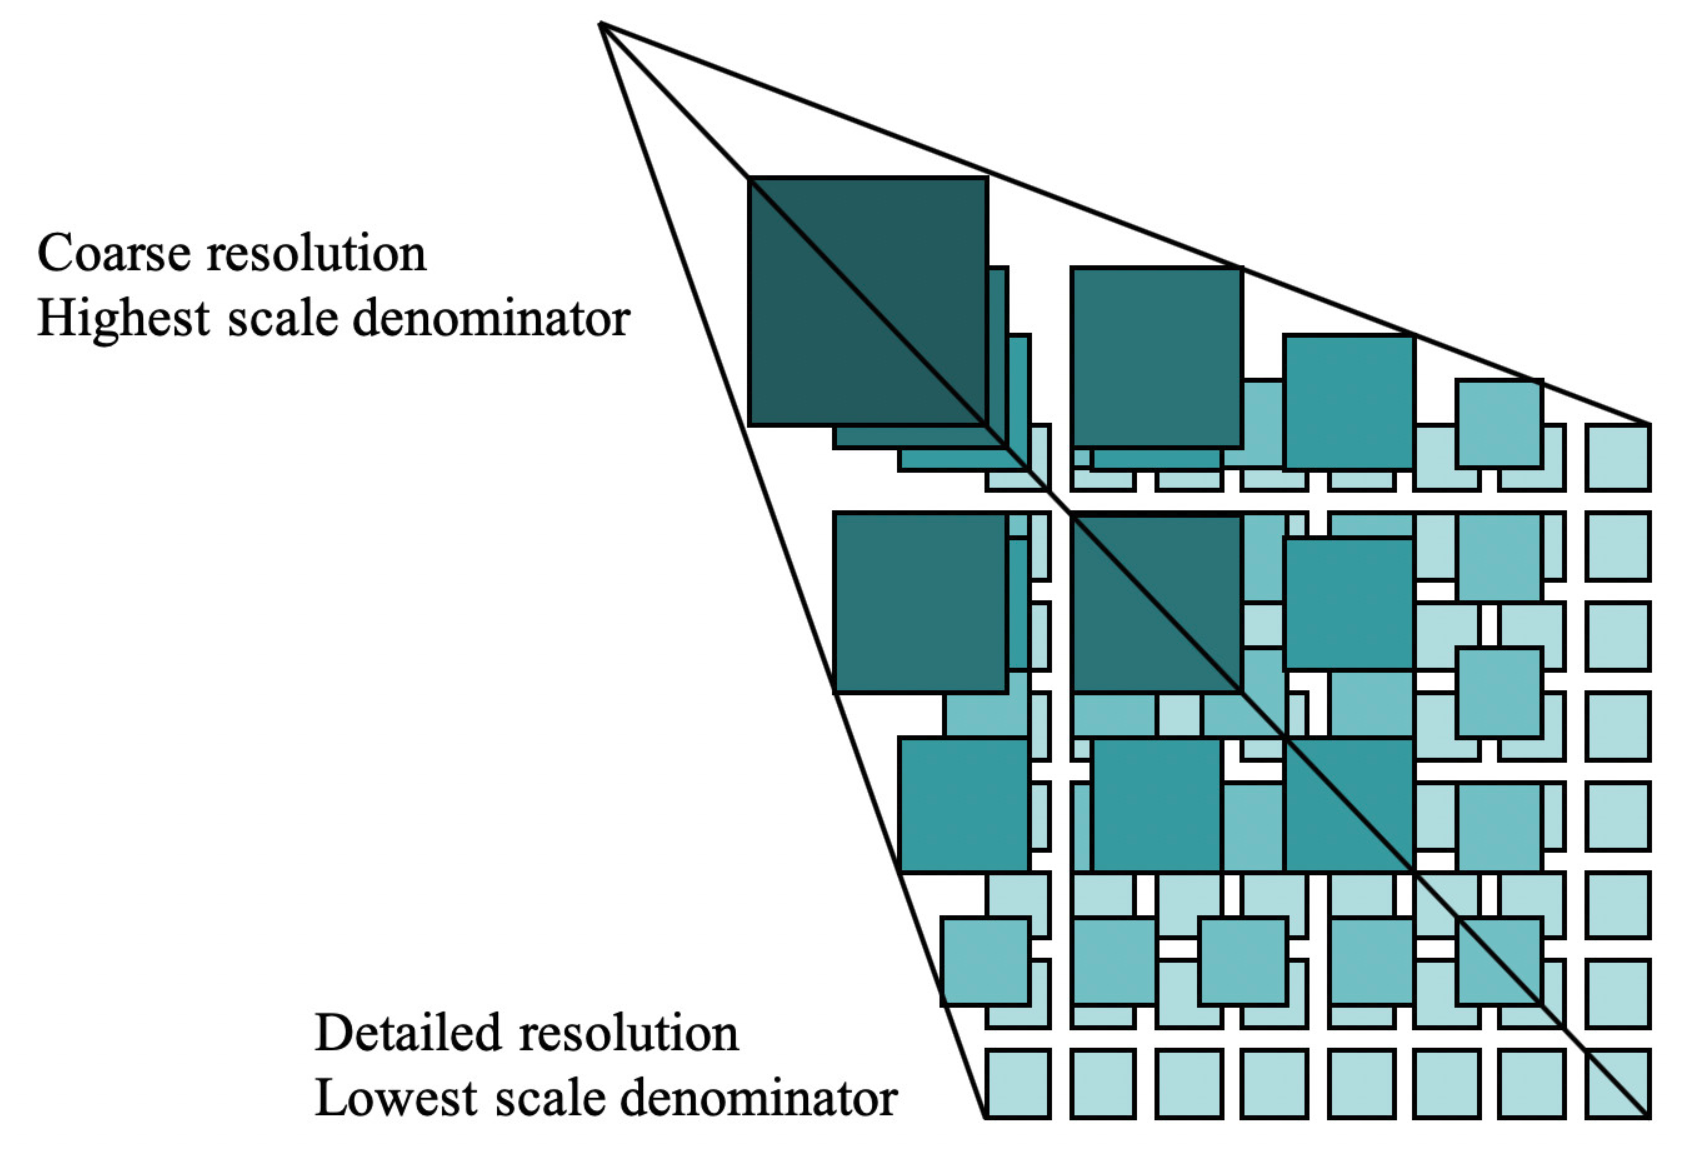
\includegraphics[width=0.7\textwidth]{figs/related_work_theoretical_bg/tms.png}
  \caption{Tile Map Service (TMS) standard for tiling geospatial data, derived from \citet{tms}}
  \label{fig:tms}
\end{figure}

When incorporating these strategies, the optimisation approaches that enable on-demand access to geospatial data are collectively referred to as \emph{cloud-optimised} formats \citep{cloud-optimised-formats}. The properties and related work of these cloud-optimised geospatial formats are discussed in detail in \autoref{rw:cloud_optimised_formats}.

\section{Binary file}
\label{tb:binary_file}
Binary file represents a fundamental approach to data storage that uses sequences of bits rather than human-readable text. Unlike plain text files that consist of characters interpreted through common character sets like ASCII, binary files store data in a format optimised for machine processing \citep{binary_file}.

Binary encoding offers several key advantages: superior storage efficiency through data compression and faster program execution. Binary files are commonly used for images, audio, executable programs, and compressed data.
However, binary encoding presents notable challenges. Binary files are not human-readable, making debugging, correction, or modification complex without specialised tools. Many binary systems are proprietary and platform-specific, creating portability issues and potential long-term accessibility problems. The Unix philosophy advocates for plain text storage when practical, emphasising that text serves as a universal interface enabling efficient program interoperability \citep{binary_file}.

In geospatial domains, prominent examples of text-based formats include GeoJSON \citep{geojson} and Geography Markup Language (GML) \citep{gml} as text representations for general geospatial data. For 3D city model data specifically, CityGML \citep{CityGML} and CityJSON \citep{cityjson} (including its streaming variant CityJSONSeq \citep{ledoux_2024}) represent the primary text-based standards. Conversely, binary geospatial formats include GeoPackage \citep{geopackage} and GeoTIFF \citep{geotiff}. Notably, no widely adopted standard binary formats currently exist for 3D city model data, representing a gap that this research aims to address.

\section{WebAssembly}
\label{tb:webassembly}
WebAssembly (WASM) is a low-level assembly-like language with a compact binary format that enables near-native performance execution in modern web browsers \citep{WebAssembly}. Standardised by the W3C \citep{WebAssemblyCoreSpecification1, WebAssemblyCoreSpecification2}, WebAssembly provides a compilation target for languages such as C/C++, C\#, and Rust, allowing code written in these languages to run efficiently on the web platform.

WebAssembly is designed to complement and run alongside JavaScript rather than replace it. Through the WebAssembly JavaScript APIs, developers can load WebAssembly modules into JavaScript applications and share functionality between the two environments \citep{WebAssembly}. This interoperability enables developers to leverage WebAssembly's performance characteristics for computationally intensive tasks while maintaining JavaScript's expressiveness and flexibility for application logic and user interface development.

A key advantage of WebAssembly is its ability to enable code reuse across platforms. Developers can compile existing codebases written in languages like C/C++, Rust, and C\# for browser deployment, eliminating the need to rewrite performance-critical components in JavaScript.

In this research, WebAssembly enables the compilation of Rust libraries for 3D city model processing to run with near-native performance in web browsers. This approach bridges the performance gap between desktop and web-based geospatial applications while maintaining the accessibility and cross-platform benefits of web deployment.

\section{Row-based and column-based data storage}
\label{tb:row_based_column_based_data_storage}

Data storage systems can be broadly categorised into two fundamental approaches: row-based and column-based storage. Row-based storage stores consecutive rows of a table sequentially, while column-based storage stores consecutive columns of a table sequentially \citep{clickhouse_column}.

To illustrate this distinction, consider the following example table:

\begin{verbatim}
id, city, country
1, Tokyo, Japan
2, London, UK
3, Amsterdam, Netherlands
\end{verbatim}

Row-based storage organises the data sequentially by rows:

\begin{verbatim}
1, Tokyo, Japan, 2, London, UK, 3, Amsterdam, Netherlands
\end{verbatim}

Column-based storage organises the data sequentially by columns:

\begin{verbatim}
1, 2, 3, Tokyo, London, Amsterdam, Japan, UK, Netherlands
\end{verbatim}

These different storage approaches exhibit distinct performance characteristics depending on the query patterns. Row-based approaches perform well for single-row searches, such as querying the record for Amsterdam. Conversely, column-based approaches excel at analytical queries that involve aggregating or filtering columns \citep{clickhouse_column}.

\citet{abadi_2008} provides a comprehensive comparison of column-stores versus row-stores, highlighting that column-based storage offers advantages in terms of storage efficiency and query performance for analytical workloads, while row-based storage is more suitable for Online Transaction Processing (OLTP) systems that require frequent lookups and updates.

In the context of geospatial data, column-based storage is particularly well-suited for analytical queries such as calculating the average height of buildings in a city or filtering buildings by construction year. However, row-based storage remains preferable for frequently updated datasets or transactional systems where individual records are accessed and modified regularly.
\section{CPU Caches}
\label{tb:cache}
Modern computing systems face a fundamental challenge to software performance due to the disparity between the speed of Central Processing Units (CPUs) and the latency of main memory. CPUs operate at clock speeds that far exceed the access speeds of dynamic random-access memory (DRAM), which typically serves as main memory. Consequently, the CPU frequently idles while waiting for data from the slower memory subsystem. To mitigate this performance bottleneck, CPU caches were developed. These caches utilise a small amount of very fast Static RAM (SRAM) to store temporary copies of data and instructions that are likely to be used again soon \citep{drepper_2007}.

The effectiveness of CPU caches hinges on two fundamental principles of program behaviour: temporal locality and spatial locality. Temporal locality refers to the tendency of a program to access data that has been recently accessed again in the near future. Spatial locality refers to the tendency of a program to access data that is located nearby in memory to previously accessed data. In other words, small chunks of data that have been accessed recently or are located nearby in memory are likely to be accessed again soon. Modern processors employ multiple levels of caches to maximise the effectiveness of these principles. This hierarchy typically consists of L1, L2, L3 caches, and main memory. The lower levels of the cache hierarchy are faster and smaller, while the higher levels are slower and larger \citep{drepper_2007}.

Data is not loaded into caches byte by byte. Instead, it is loaded in blocks called cache lines, typically 64 bytes in size. This design reduces the number of separate memory transactions and effectively amortises the substantial latency involved in accessing main memory \citep{drepper_2007}.

The performance of a cache is fundamentally determined by its hit rate. A cache hit occurs when the requested data is found within the cache, resulting in very fast access. In contrast, a cache miss occurs when the requested data is not found within the cache, necessitating a much slower retrieval from a higher-level cache or, in the worst case, main memory \citep{abayomi_2020}.

Understanding these aspects of cache behaviour is crucial when designing binary data formats, as cache-friendly data layouts can significantly improve application performance.

\section{Serialisation and Deserialisation}
\label{tb:serialisation_deserialisation}
Before discussing the specific techniques used in the FlatCityBuf format, it is important to understand the general principles of serialisation and deserialisation.

The terminology for data conversion processes varies across different programming ecosystems. Terms such as serialisation, pickling, marshalling, and flattening are often used interchangeably, though with subtle differences depending on the context. \citet{cpp_serialization} describes it from an object-oriented perspective as converting objects in memory (in a data structure) to a storable or transmittable format on disk. \citet{py_serialization} refers to this process as "pickling" in the Python ecosystem. For clarity in this thesis, we adopt the definition provided by \citet{viotti_2022}:

\begin{quote}
  "Serialisation is the process of translating a data structure into a bit-string (a sequence of bits) for storage or transmission purposes."
\end{quote}

Deserialisation is the reverse process of serialisation, where the bit-string is converted back into the original data structure (in memory).

\section{Zero-copy}
\label{tb:zero_copy}
Zero-copy is a technique used to avoid copying data from one memory location to another. The term "Zero-copy" is used in many contexts of computer science, \citet{song2012performance}  and \citet{brose_2008_zerocopy} provide a detailed explanation of the concept.

In conventional I/O operations, data typically traverses multiple memory regions, each requiring a separate copy operation:

\begin{itemize}
  \item Data is copied from storage devices into kernel buffer cache
  \item From kernel buffer, data is copied to user-space application buffers
  \item For network transmission, data may be copied again to network buffers
\end{itemize}

This multi-stage copying introduces significant overhead, particularly for large datasets or high-throughput applications. Each copy operation consumes CPU cycles, memory bandwidth, and increases latency \citep{song2012performance}. For applications working with large 3D city models, this overhead can substantially degrade performance.

\todo{Todo: improve here}
Zero-copy approaches optimise this data path by eliminating unnecessary copy operations. While "zero-copy" as a term suggests complete elimination of copying, in practice, different techniques achieve varying degrees of copy reduction:

\begin{itemize}
  \item \textbf{Memory-mapped \ac{io}}: Maps files directly into process address space, allowing direct access without explicit read/write operations
  \item \textbf{Direct \ac{io}}: Bypasses the kernel buffer cache for specific workloads
  \item \textbf{Scatter-gather \ac{io}}: Reads data directly into discontiguous memory regions
  \item \textbf{Shared memory}: Provides common address space for inter-process communication
  \item \textbf{In-place parsing}: Processes data structures without creating intermediate copies
\end{itemize}
\todo{ravi's comment "so this is in-place parsing, which also enables memory mapping? Are some other of the above terms also relevant? Clarify exactly how Flatbuffers relates to what you explain above."}

Modern serialisation formats like FlatBuffers implement zero-copy through carefully designed memory layouts that allow direct access to serialised data without requiring a separate deserialisation step. This approach is particularly valuable for geospatial applications that routinely handle large datasets.
\section{Endianness}
\label{tb:endianness}
Endianness (or "byte-order") refers to the order in which bytes are stored in memory when representing multi-byte values. The terminology was introduced by \citet{danny_cohen_1981}.

In computing, endianness becomes significant when multi-byte data types (such as 16-bit integers or 32-bit floats) must be stored in memory or transmitted across networks. There are two primary byte ordering systems:

\begin{itemize}
  \item \textbf{Little-endian}: Stores the least significant byte at the lowest memory address, followed by increasingly significant bytes. This is the ordering used by Intel processors that dominate desktop and server computing. For example, the 32-bit integer \texttt{0x12345678} would be stored in memory as 4 bytes: \texttt{0x78}, \texttt{0x56}, \texttt{0x34}, \texttt{0x12}.

  \item \textbf{Big-endian}: Stores the most significant byte at the lowest memory address. This approach is often called ``network byte order'' because Internet protocols typically require data to be transmitted in big-endian format. For example, the same 32-bit integer \texttt{0x12345678} would be stored as \texttt{0x12}, \texttt{0x34}, \texttt{0x56}, \texttt{0x78}.
\end{itemize}

A useful analogy is date notation: little-endian resembles the European date format (31 December 2050), while big-endian resembles the ISO format (2050-12-31), with the most significant part (year) first \citep{endianness_mdn}.

\section{Binary Search}
\label{tb:binary_search}

Binary search is a fundamental algorithm for finding elements in a sorted array. The classic implementation follows a simple approach: compare the search key with the middle element of the array, then recursively search the left or right half depending on the comparison result \citep{binary_search}.

The time complexity of binary search is logarithmic—the height of the implicit binary search tree is $\log_2(n)$ for an array of size $n$. While this is theoretically efficient, the actual performance suffers when implemented on modern hardware due to memory access patterns. Each comparison requires the processor to fetch a new element, potentially causing a cache miss (cache miss is explained in \autoref{tb:cache}). In the worst case, the number of memory read operations will be proportional to the height of the tree, with each read potentially requiring access to a different cache line or disk block \citep{binary_search}.

This inefficiency is particularly problematic when binary search is implemented on external memory or over HTTP, where each access incurs significant latency. The sorted array representation with binary search does not take advantage of CPU cache locality, as consecutive comparisons frequently access distant memory locations.

\subsection{Eytzinger Layout}
\label{tb:eytzinger_layout}

While preserving the same algorithmic idea as binary search, the Eytzinger layout (also known as a complete binary tree layout or level-order layout) rearranges the array elements to match the access pattern of a binary search \citep{binary_search}. Instead of storing elements in sorted order, it places them in the order they would be visited during a level-order traversal of a complete binary tree.

This layout significantly improves memory access patterns. When the array is accessed in the sequence of a binary search operation, adjacent accesses often refer to elements that are in the same or adjacent cache lines. This layout also proves beneficial for managing data fetched over networks, as consecutive elements accessed during binary search are more likely to be retrieved in the same HTTP range request, thereby reducing the number of network roundtrips and overall latency. This spatial locality enables effective hardware prefetching, allowing the CPU to anticipate and load required data before it is explicitly accessed, thus reducing latency \citep{binary_search}.

\autoref{fig:eytzinger_layout} shows how the layout appears when applied to binary search. \autoref{fig:eytzinger_layout2} shows that the algorithm starts from the first element and then jumps to either $2k$ or $2k+1$ depending on the comparison result. The heatmap represents the expected frequency of comparisons for search (the closer to the top, the more frequent the comparison).

\begin{figure}[ht]
  \centering
  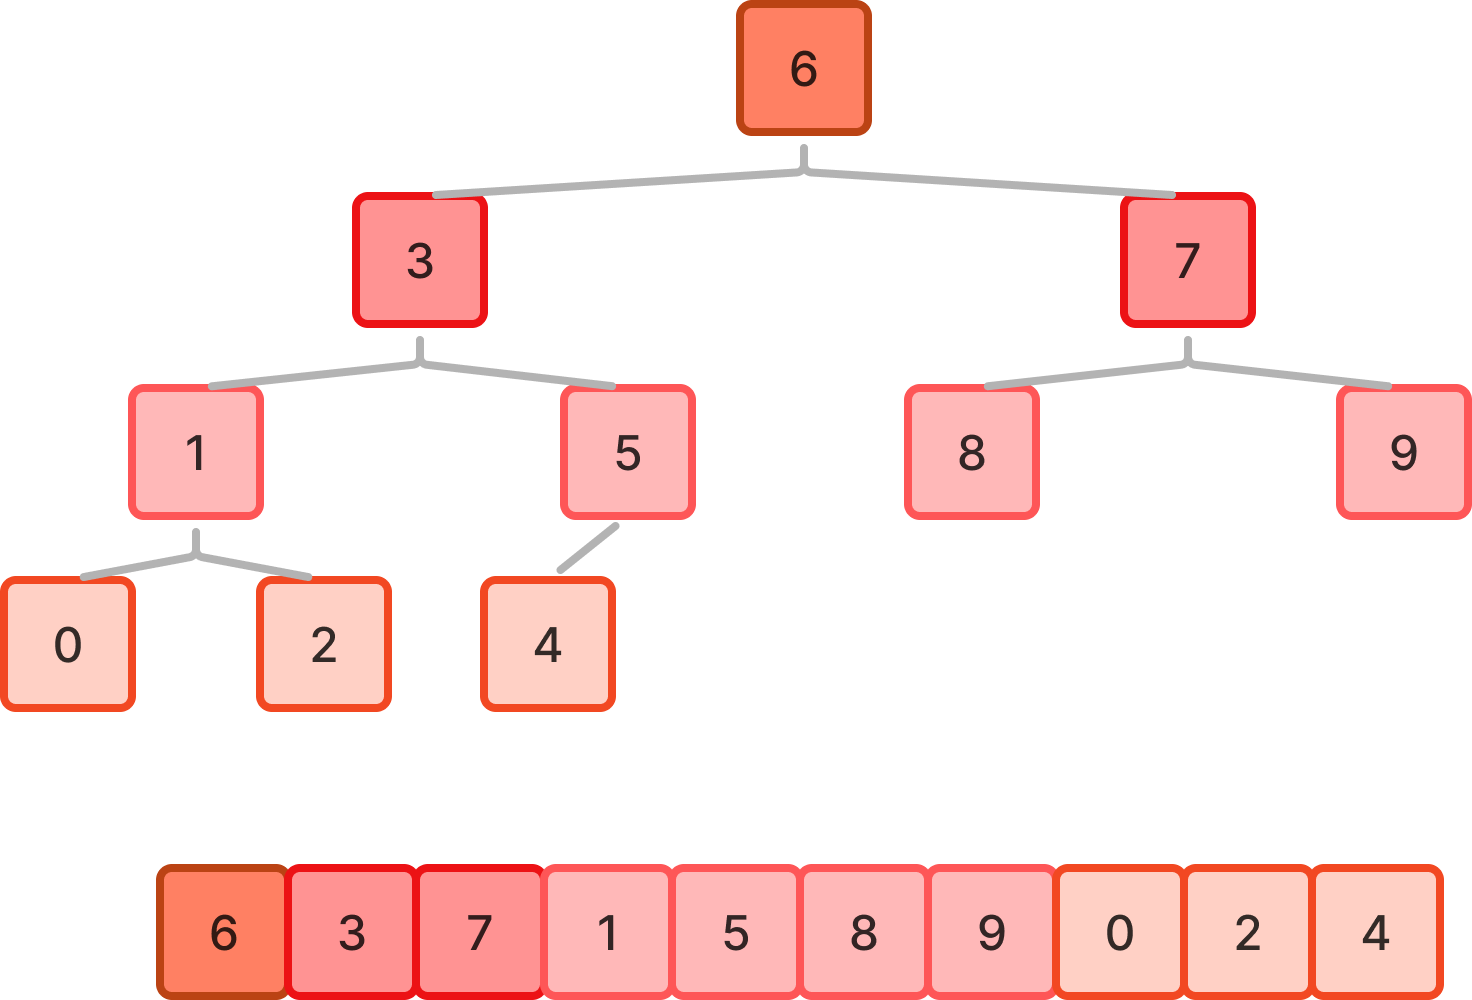
\includegraphics[width=0.5\textwidth]{figs/related_work_theoretical_bg/eytzinger_layout.png}
  \caption{Eytzinger layout as conceptual representation as tree and actual data layout (modified from \citet{binary_search})}
  \label{fig:eytzinger_layout}
\end{figure}
\begin{figure}[ht]
  \centering
  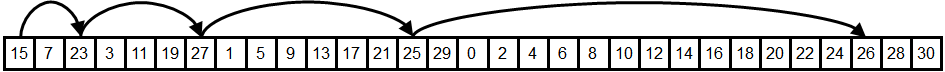
\includegraphics[width=0.5\textwidth]{figs/related_work_theoretical_bg/eytzinger_layout2.png}
  \caption{Binary search traversal pattern in Eytzinger layout (modified from \citet{binary_search})}
  \label{fig:eytzinger_layout2}
\end{figure}

\section{\texorpdfstring{\ac{s+tree}}{S+tree}}
\label{tb:static_btree}

\subsection{B-Tree/B+Tree Layout}
\label{tb:btree_layout}

While the Eytzinger layout improves cache utilisation for binary search, the number of memory read operations remains proportional to the height of the tree—$\log_2(n)$ for $n$ elements. This is still suboptimal for large datasets, especially when the access pattern involves disk \ac{io} or remote data access \citep{static_b_trees}.

B-Trees and their variants address this limitation by storing multiple keys in each node, effectively reducing the height of the tree. In a B-Tree of order $k$ (where each node can contain up to $k-1$ keys), the height of the tree is reduced from $\log_2(n)$ to $\log_k(n)$. This represents a reduction factor of $\log_k/\log_2 = \log_2(k)$ times compared to a binary search tree.

The key insight is that fetching a single node still takes roughly the same time regardless of whether it contains one key or multiple keys, as long as the entire node fits into a single memory block or disk page. By packing multiple keys into each node, B-Trees significantly reduce the number of disk or memory accesses required to locate an element.

B+Trees are a variant of B-Trees specifically optimised for range queries and sequential access patterns. In a B+Tree:
\begin{itemize}
  \item Internal nodes contain up to $B$ keys that serve as routing information, with each key associated with one of the $(B+1)$ pointers to child nodes. Each key at position $i$ represents the smallest key in the subtree pointed to by the $(i+1)$-th child pointer.
  \item Leaf nodes store the actual data with up to $B$ key-value pairs and include a pointer to the next leaf node, enabling efficient sequential traversal for range queries.
\end{itemize}

This linked structure of leaf nodes enables B+Trees to efficiently support range queries by traversing from one leaf to the next without needing to return to higher levels of the tree.

As the figure \ref{fig:btree_bplus_tree} shows, the B+Tree has pointers to the next leaf node, which enables efficient sequential traversal for range queries. On the other hand, the B+Tree has duplicate keys in the internal nodes, which is not the case for the B-Tree.

\begin{figure}[ht]
  \centering
  \begin{subfigure}[b]{0.45\textwidth}
    \centering
    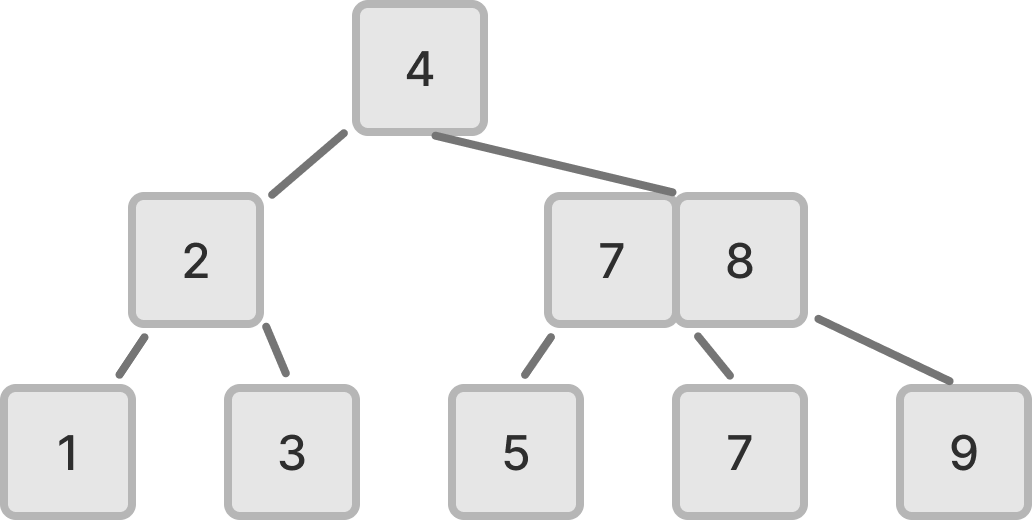
\includegraphics[width=\textwidth]{figs/related_work_theoretical_bg/btree.png}
    \caption{B-Tree (branching factor 3)}
    \label{fig:btree}
  \end{subfigure}
  \hfill
  \begin{subfigure}[b]{0.45\textwidth}
    \centering
    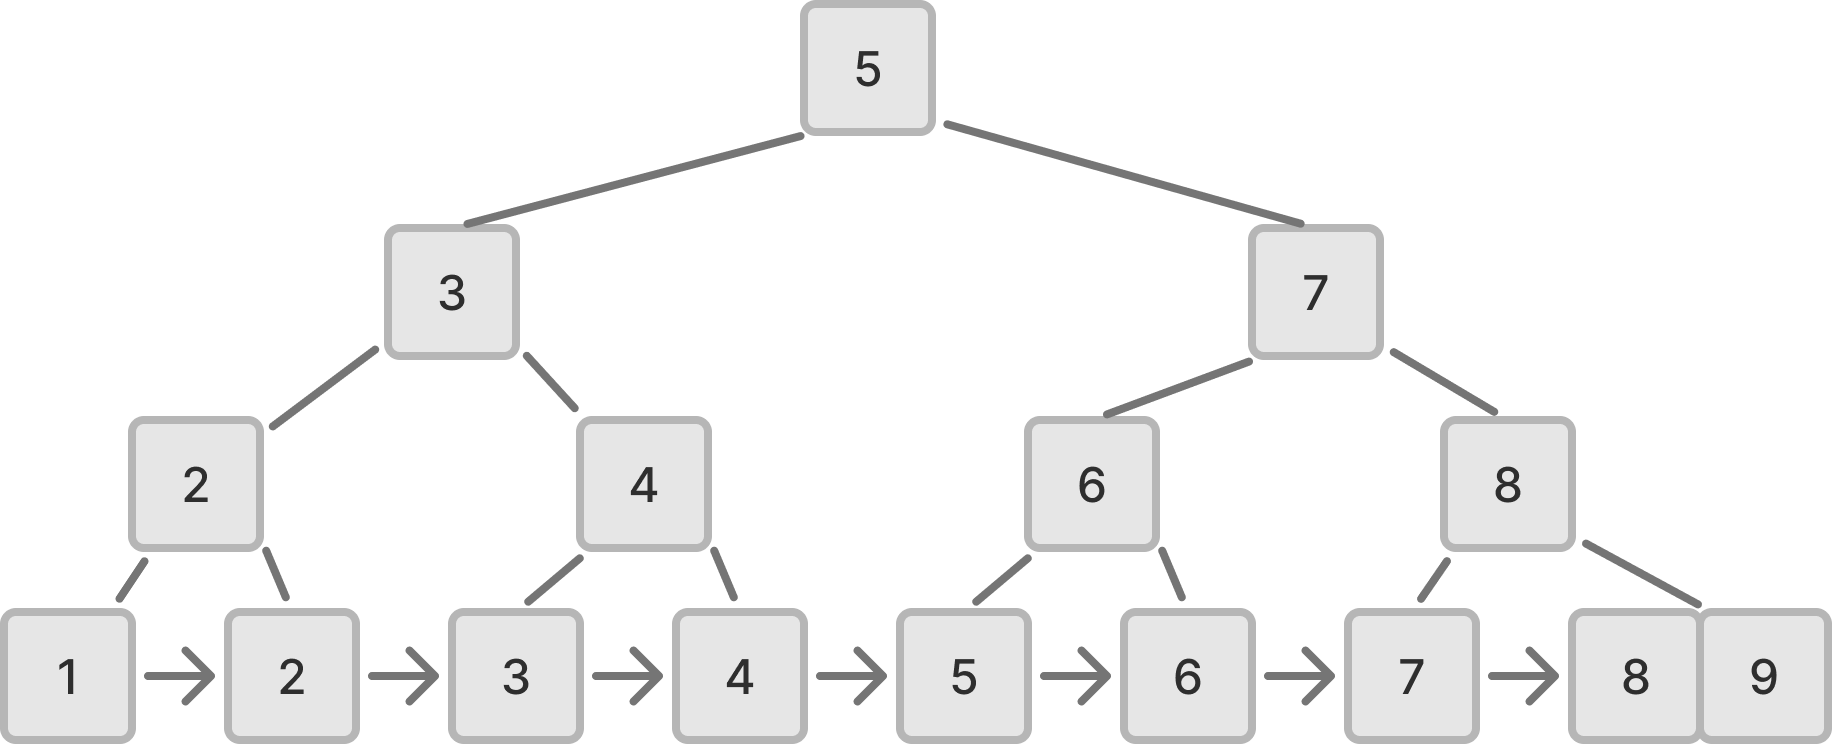
\includegraphics[width=\textwidth]{figs/related_work_theoretical_bg/bplus_tree.png}
    \caption{B+Tree (branching factor 3)}
    \label{fig:bplus_tree}
  \end{subfigure}
  \caption{B-Tree and B+Tree}
  \label{fig:btree_bplus_tree}
\end{figure}

\subsection{\texorpdfstring{\ac{s+tree}}{S+tree}}
\label{tb:stree}

The S+Tree (Static B+Tree), introduced by Algorithmica \citep{static_b_trees}, builds upon the B+Tree concept but is specifically designed for static datasets where the tree structure never changes after construction. Unlike traditional B+Trees that use explicit pointers between nodes, the S+Tree uses an implicit structure where child positions are calculated mathematically.
This is possible because:
\begin{itemize}
  \item The tree is constructed once and never modified (static)
  \item The number of elements is known in advance
  \item The tree can be maximally filled with no empty slots
  \item Child positions follow a predictable pattern based on the block size
\end{itemize}

For a \ac{s+tree} with block size $B$, a node with index $k$ has its children at indices calculated by a simple formula: $\text{child}_i(k) = k \cdot (B+1) + i + 1$ for $i \in [0, B]$ \citep{static_b_trees}. This eliminates the need to store and fetch explicit pointer values, further reducing memory usage and improving cache efficiency.

The S+Tree layout aligns with modern hardware characteristics where:
\begin{itemize}
  \item The latency of fetching a single byte is comparable to fetching an entire cache line (64 bytes)
  \item Disk and network I/O operations have high initial latency but relatively low marginal cost for additional bytes
  \item CPU cache lines typically hold multiple array elements (e.g., 16 integers in a 64-byte cache line)
\end{itemize}

By loading a block of $B$ elements at once and performing a local search within that block, S+Trees reduce the total number of cache misses or disk accesses to $\log_B(n)$ instead of $\log_2(n)$—a significant reduction for large datasets.

The S+Tree layout achieves up to 15× performance improvement over standard binary search implementations while requiring only 6-7\% additional memory \citep{static_b_trees}. This makes it particularly valuable for applications that perform frequent searches on large, relatively static datasets, especially when accessed over high-latency connections. For more detailed implementation strategies of S+Tree, \citet{koerkamp_2024} provides comprehensive explanations and practical considerations.
%!TEX root = ../../thesis.tex

\section{FlatBuffers Framework}
\label{rw_tb:fb}

FlatBuffers, developed by \citet{flatbuffers}, is a cross-platform serialisation framework designed specifically for performance-critical applications with a focus on memory efficiency and processing speed. Unlike traditional serialisation approaches, FlatBuffers implements a zero-copy deserialisation mechanism that enables direct access to serialised data without an intermediate parsing step \citep{flatbuffers_benchmark}, as discussed in \autoref{tb:zero_copy}. This characteristic is particularly advantageous for large geospatial datasets where parsing overhead can significantly impact performance.

\subsection{Schema-Based Serialisation}
\label{rw_tb:fb:schema_based_serialisation}

FlatBuffers employs a strongly typed, schema-based approach to data serialisation. The workflow involves:

\begin{enumerate}
    \item Definition of data structures in schema files with the \texttt{.fbs} extension
    \item Compilation of schema files using the FlatBuffers compiler (\texttt{flatc})
    \item Generation of language-specific code for data access
    \item Implementation of application logic using the generated code
\end{enumerate}

This schema-first approach enforces data consistency and type safety, which is essential to be processed in various programming languages and environments. The generated code provides memory-efficient access patterns to the underlying binary data without requiring full deserialisation. FlatCityBuf utilises this capability to achieve a balance between parsing speed and storage efficiency.

The FlatBuffers compiler supports code generation for multiple programming languages, including C++, Java, C\#, Go, Python, JavaScript, TypeScript, Rust, and others, facilitating cross-platform interoperability \citep{flatbuffers_support}. This extensive language support enables developers to work with FlatBuffers data in their preferred environment. For FlatCityBuf, Rust was selected as the primary implementation language due to its performance characteristics and memory safety guarantees.

\subsection{Data Type System}
\label{rw_tb:fb:data_type_system}

FlatBuffers provides a comprehensive type system that balances efficiency and expressiveness \citep{flatbuffers_data_types}:

\begin{itemize}
  \item \textbf{Tables}: Variable-sized object containers that support:
    \begin{itemize}
      \item Named fields with type annotations
      \item Optional fields with default values
      \item Schema evolution through backward compatibility
      \item Non-sequential field storage for memory optimisation
    \end{itemize}

  \item \textbf{Structs}: Fixed-size, inline aggregates that:
    \begin{itemize}
      \item Require all fields to be present (no optionality)
      \item Are stored directly within their containing object
      \item Provide faster access at the cost of schema flexibility
      \item Optimise memory layout for primitive types
    \end{itemize}

  \item \textbf{Scalar Types}:
    \begin{itemize}
      \item 8-bit integers: \texttt{byte} (int8), \texttt{ubyte} (uint8), \texttt{bool}
      \item 16-bit integers: \texttt{short} (int16), \texttt{ushort} (uint16)
      \item 32-bit values: \texttt{int} (int32), \texttt{uint} (uint32), \texttt{float}
      \item 64-bit values: \texttt{long} (int64), \texttt{ulong} (uint64), \texttt{double}
    \end{itemize}

  \item \textbf{Complex Types}:
    \begin{itemize}
      \item \texttt{[T]}: Vectors (single-dimension arrays) of any supported type
      \item \texttt{string}: UTF-8 or 7-bit ASCII encoded text with length prefix
      \item References to other tables, structs, or unions
    \end{itemize}

  \item \textbf{Enums}: Type-safe constants mapped to underlying integer types
  \item \textbf{Unions}: Tagged unions supporting variant types
\end{itemize}

\subsection{Schema Organisation Features}
\label{rw_tb:fb:schema_organisation}

In addition to the data type system, FlatBuffers provides several key features for organising complex schemas:

\begin{itemize}
  \item \textbf{Namespaces} (\texttt{namespace FlatCityBuf;}) create logical boundaries and prevent naming collisions

  \item \textbf{Include Mechanism} (\texttt{include "header.fbs";}) enables modular schema design across multiple files

  \item \textbf{Root Type} (\texttt{root\_type Header;}) identifies the primary table that serves as the entry point for buffer access
\end{itemize}

These features were essential for FlatCityBuf's implementation, enabling modular schema development with separate root types for header and feature components while maintaining consistent type definitions across files.

\todo{move this section to theoretical background?}
\subsection{Binary Structure and Memory Layout}
\label{rw_tb:fb:binary_structure}

FlatBuffers organises serialised data in a flat binary buffer with the following characteristics:

\begin{itemize}
    \item \textbf{Prefix-based vtables} that enable field access without full parsing
    \item \textbf{Offset-based references} that allow direct navigation within the buffer
    \item \textbf{Aligned memory layout} optimised for CPU cache efficiency
    \item \textbf{Endian-aware serialisation} supporting both little and big-endian platforms
\end{itemize}

For complex data structures like 3D city models, FlatBuffers allows for modular schema composition through file inclusion. This capability enabled the separation of FlatCityBuf's schema into logical components (\texttt{header.fbs}, \texttt{feature.fbs}, \texttt{geometry.fbs}, etc.) while maintaining efficient serialisation. In our implementation, the \texttt{Header} and \texttt{CityFeature} tables serve as root types that anchor the overall data structure.


% Methodology-----------------------
%!TEX root = ../../thesis.tex

\chapter{Methodology}
\label{methodology}

This chapter presents the design and implementation of FlatCityBuf, a cloud-optimised binary format for 3D city models based on CityJSONSeq. The proposed approach addresses the limitations of existing formats through efficient binary encoding, spatial indexing, attribute indexing, and support for partial data retrieval.

\section{Overview}
\label{methodology:overview}

\subsection{Methodology Approach}
\label{methodology:overview:approach}

Current 3D city model formats like CityGML, CityJSON, and \ac{cjseq} exhibit limitations in cloud environments with large-scale datasets, including retrieval latency, inefficient spatial querying without additional software support, and insufficient support for partial data access.

This chapter addresses these limitations through three interconnected objectives:

\begin{enumerate}
  \item Development of a binary encoding strategy using FlatBuffers that preserves semantic richness while achieving faster read performance
  \item Implementation of dual indexing mechanisms—spatial (packed Hilbert R-tree) and attribute-based (\ac{s+tree}) that accelerate query performance
  \item Integration of cloud-native data access patterns through HTTP Range Requests, enabling partial data retrieval
\end{enumerate}

\subsection{Outcomes of the Methodology}
\label{methodology:overview:outcomes}

Before delving into the methodological details, it is important to highlight the tangible research outcomes produced through this work:

\begin{itemize}
  \item \textbf{Data format specification}: FlatCityBuf, a cloud-optimised binary format for 3D city models that maintains semantic compatibility with CityJSON while enabling efficient cloud-based access patterns.

  \item \textbf{Reference implementation}: A comprehensive Rust library for encoding, decoding, and querying FlatCityBuf files, accompanied by command-line interface (CLI) tools for conversion and validation.

  \item \textbf{Web demonstration}: A web-based prototype application that showcases the partial data retrieval capabilities of FlatCityBuf through HTTP range requests, demonstrating practical performance improvements in real-world scenarios.

  \item \textbf{Performance evaluation}: A comprehensive performance evaluation of the proposed methodology, demonstrating the benefits of the proposed approach in terms of file size, query latency, memory usage, and other relevant metrics.
\end{itemize}

These outcomes collectively address the research objectives by providing both a theoretical framework and practical implementations that validate the approach to cloud-optimised 3D city model storage and retrieval.

\subsection{File Structure Overview}
\label{methodology:overview:file_structure}

The FlatCityBuf format implements a structured binary encoding with five sequentially arranged components:

\begin{itemize}
  \item \textbf{Magic bytes}: Eight-byte identifier ('F', 'C', 'B', '0', '1', '0', '0', '0') for format validation
  \item \textbf{Header section}: Contains metadata, attributes schema definitions, and CityJSON properties
  \item \textbf{Spatial index}: Implements a Packed Hilbert R-tree \citep{Kamel_Faloutsos_1993} for efficient geospatial queries
  \item \textbf{Attribute index}: Utilises a \ac{s+tree} for accelerated attribute-based filtering
  \item \textbf{Features section}: Stores features encoded as FlatBuffers tables
\end{itemize}

\begin{figure}[h]
  \centering
  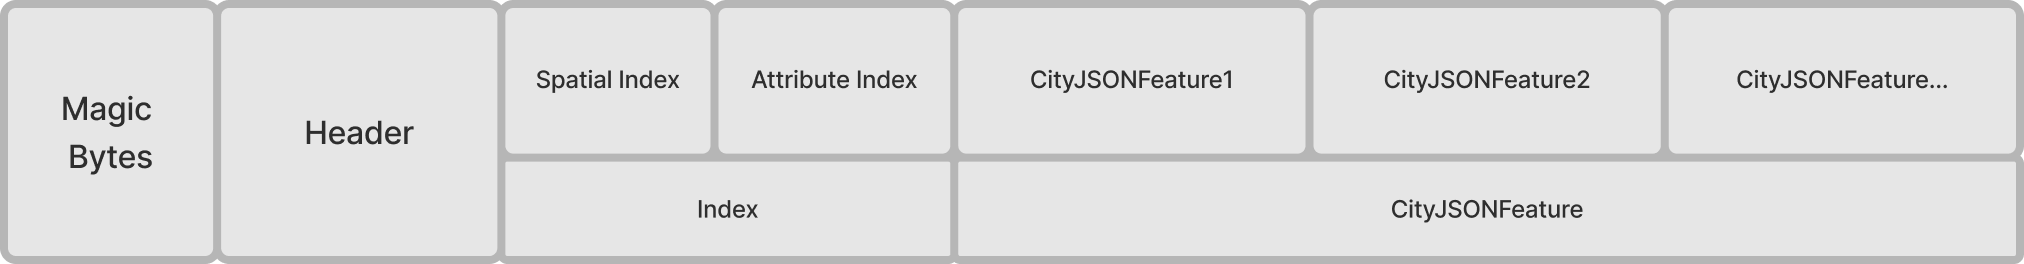
\includegraphics[width=0.8\textwidth]{figs/methodology/file_structure.png}
  \caption{Physical layout of the FlatCityBuf file format, showing section boundaries and alignment considerations for optimised range requests}
  \label{fig:methodology:file-structure}
\end{figure}

This sequence-based structure enables incremental file access through HTTP Range Requests—critical for cloud-based applications where minimising data transfer is essential.

\subsection{Note on Binary Encoding}
\label{methodology:overview:note_on_binary_encoding}
\todo{add reference why these two}
FlatCityBuf follows two key conventions for encoding binary data throughout the file format:

\begin{enumerate}
  \item \textbf{Size-prefixed FlatBuffers}: All FlatBuffers records (header and features) include a 4-byte unsigned integer prefix indicating the buffer size. This enables programs to know the size of the record without parsing the entire content. The FlatBuffers API implements this through \texttt{finish\_size\_prefixed} or equivalent language-specific methods.
  \item \textbf{Little-endian encoding}: For data encoded outside FlatBuffers records (particularly in spatial and attribute indices), little-endian byte ordering is consistently applied, matching the endianness convention used within FlatBuffers records. This includes numeric values such as 32-bit and 64-bit integers, floating-point numbers, and offset values within indices.
\end{enumerate}

\todo{add reference}
These conventions ensure consistency across the file format and maximise compatibility with modern CPU architectures, most of which use little-endian byte ordering. The size-prefixing mechanism is particularly important for cloud-based access patterns, as it facilitates precise HTTP Range Requests when retrieving specific file segments.


\section{Magic Bytes}
\label{methodology:file_components:magic_bytes}

The magic bytes section comprises the first eight bytes of the file:
\todo{check detail again}
\begin{itemize}
  \item The first four bytes contain the ASCII sequence 'FCB\\0' (0x46 0x43 0x42 0x00) serving as an immediate identifier
  \item The remaining four bytes follow a pattern similar to FlatGeoBuf \citep{flatgeobuf}, with byte 5-6 containing major version (currently 01), followed by ASCII 'FB' (0x46 0x42), and byte 8 containing patch version (currently 00)
\end{itemize}

This signature design enables applications to validate file type and version compatibility without parsing the entire header content.

\section{Header Section}
\label{methodology:file_components:header}

The header section encapsulates metadata essential for interpreting the file contents, implemented as a size-prefixed FlatBuffers-serialised \texttt{Header} table. The header serves a dual purpose: it maintains compatibility with CityJSON by encoding the equivalent of the first line of a CityJSONSeq stream \citep{ledoux_2024}—which contains the root CityJSON object with metadata, coordinate reference system, and transformations—while adding FlatCityBuf-specific extensions for optimised retrieval and indexing. The full schema definition for the header can be found in \autoref{appendix:flatcitybuf_schema}.

In a CityJSONSeq file, the first line contains a valid CityJSON object with empty \texttt{CityObjects} and \texttt{vertices} arrays but with essential global properties like \texttt{transform}, \texttt{metadata}, and \texttt{version}. The FlatCityBuf header encodes these same properties alongside additional indexing information required for cloud-optimised access patterns.

\subsection{CityJSON Metadata Fields}
\label{methodology:header:cityjson_fields}

Here are the core header fields with their data types and significance:

\begin{itemize}
  \item \textbf{version} - \textit{string (required)} - CityJSON version identifier (\eg, "2.1"), required field from CityJSON specification \citep{cityjson_spec}

  \item \textbf{transform} - \textit{Transform struct} - Contains scale and translation vectors enabling efficient storage of vertex coordinates through quantization, derived from CityJSON's transform object \citep{cityjson_spec}

  \item \textbf{reference\_system} - \textit{ReferenceSystem table} - Coordinate reference system information including:
    \begin{itemize}
      \item \textit{authority} - Authority name, typically "EPSG"
      \item \textit{code} - Numeric identifier of the CRS
      \item \textit{version} - Version of the CRS definition
    \end{itemize}

  \item \textbf{geographical\_extent} - \textit{GeographicalExtent struct} - 3D bounding box containing min/max coordinates for the dataset \citep{cityjson_spec}

  \item \textbf{identifier} - \textit{string} - Unique identifier for the dataset

  \item \textbf{title} - \textit{string} - Human-readable title for the dataset

  \item \textbf{reference\_date} - \textit{string} - Date of reference for the dataset

  \item \textbf{point of contact} - Contact information for the dataset provider \citep{cityjson_spec}:
    \begin{itemize}
      \item \textit{poc\_contact\_name} - Name of the point of contact
      \item \textit{poc\_contact\_type} - Type of contact (\eg, "individual", "organization")
      \item \textit{poc\_role} - Role of the contact (\eg, "author", "custodian")
      \item \textit{poc\_email} - Email address of the contact
      \item \textit{poc\_website} - Website for the contact
      \item \textit{poc\_phone} - Phone number of the contact
      \item \textit{poc\_address\_*} - Address components including thoroughfare number, name, locality, postcode, country
    \end{itemize}
\end{itemize}


\subsection{Appearance Information}
\label{methodology:header:appearance}

Fields storing global appearance definitions:

\begin{itemize}
  \item \textbf{appearance} - \textit{Appearance table} - Container for visual representation properties, following CityJSON's appearance model \citep{cityjson_spec}, containing:
    \begin{itemize}
      \item \textit{materials} - Array of Material tables with the following properties:
        \begin{itemize}
          \item \textit{name} - Required string identifier for the material
          \item \textit{ambient\_intensity} - Double precision value from 0.0 to 1.0
          \item \textit{diffuse\_color} - Array of double values (RGB) from 0.0 to 1.0
          \item \textit{emissive\_color} - Array of double values (RGB) from 0.0 to 1.0
          \item \textit{specular\_color} - Array of double values (RGB) from 0.0 to 1.0
          \item \textit{shininess} - Double precision value from 0.0 to 1.0
          \item \textit{transparency} - Double precision value from 0.0 to 1.0
          \item \textit{is\_smooth} - Boolean flag for smooth shading
        \end{itemize}

      \item \textit{textures} - Array of Texture tables with the following properties:
        \begin{itemize}
          \item \textit{type} - TextureFormat enum (PNG, JPG)
          \item \textit{image} - Required string containing image file name or URL
          \item \textit{wrap\_mode} - WrapMode enum (None, Wrap, Mirror, Clamp, Border)
          \item \textit{texture\_type} - TextureType enum (Unknown, Specific, Typical)
          \item \textit{border\_color} - Array of double values (RGBA) from 0.0 to 1.0
        \end{itemize}

      \item \textit{vertices\_texture} - Array of Vec2 structs containing UV coordinates (u,v), each coordinate value must be between 0.0 and 1.0 for proper texture mapping

      \item \textit{default\_theme\_material} and \textit{default\_theme\_texture} - Strings identifying default themes for rendering when multiple themes are defined
    \end{itemize}
\end{itemize}

The appearance model provides a standardized way to define visual properties of city objects, supporting multiple rendering engines and visualization tools. Materials define surface properties while textures allow mapping of image data onto geometry surfaces. The separation of appearance definitions from geometry enables efficient storage by allowing multiple surfaces to reference the same materials or textures.

\subsection{Geometry Templates}
\label{methodology:header:geometry_templates}

Fields supporting geometry reuse:

\begin{itemize}
  \item \textbf{templates} - \textit{Array of Geometry tables} - Reusable geometry definitions that can be instantiated multiple times, following CityJSON's template concept \citep{cityjson_spec}

  \item \textbf{templates\_vertices} - \textit{Array of DoubleVertex structs} - Double-precision vertices used by templates, stored separately from feature vertices for higher precision in the local coordinate system \citep{cityjson_spec}
\end{itemize}

The templates mechanism enables significant storage efficiency for datasets containing repetitive structures such as standardised building designs, street furniture, or vegetation. The detailed structure of geometry encoding, including boundary representation and semantic surface classification, will be explained further in \autoref{methodology:feature_encoding}.

\subsection{Extension Support}
\label{methodology:header:extensions}

Fields enabling schema extensibility:

\begin{itemize}
  \item \textbf{extensions} - \textit{Array of Extension tables} - Definitions for CityJSON extensions \citep{cityjson_spec}, each containing:
    \begin{itemize}
      \item \textit{name} - Extension identifier (\eg, "+Noise")
      \item \textit{url} - Reference to the extension schema
      \item \textit{version} - Extension version identifier
      \item \textit{extra\_attributes}, \textit{extra\_city\_objects}, \textit{extra\_root\_properties}, \textit{extra\_semantic\_surfaces} - Stringified JSON schemas for extension components
    \end{itemize}
\end{itemize}

Unlike standard CityJSON \citep{cityjson_spec}, which references external schema definition files for extensions, FlatCityBuf embeds the complete extension schemas directly within the file as stringified JSON. This approach creates a self-contained, all-in-one data format that can be interpreted correctly without requiring access to external resources.

The embedding of extension schemas follows FlatCityBuf's design principle of maintaining file independence while preserving full compatibility with the CityJSON extension mechanism. The specific implementation details of how extended city objects and semantic surfaces are encoded in individual features will be explained further in \autoref{methodology:feature_encoding}.

\subsection{Attribute Schema and Indexing Metadata}
\label{methodology:header:schema_indexing}

Fields supporting attribute interpretation and efficient querying:

\begin{itemize}
  \item \textbf{columns} - \textit{Array of Column tables} - Schema definitions for attribute data. This metadata is used to interpret the values of the attributes in the features. Each containing:
    \begin{itemize}
      \item \textit{index} - Numeric identifier of the column
      \item \textit{name} - Name of the attribute (\eg, "cityname", "owner", \etc)
      \item \textit{type} - Data type enumeration (\eg, "Int", "String", \etc)
      \item \textit{nullable}, \textit{unique}, \textit{precision} - Optional metadata for validating and interpreting values
    \end{itemize}

  \item \textbf{features\_count} - \textit{ulong} - Total number of features in the dataset, enables client applications to pre-allocate resources

  \item \textbf{index\_node\_size} - \textit{ushort} - Number of entries per node in the spatial index, defaults to 16, tuned for typical HTTP request sizes

  \item \textbf{attribute\_index} - \textit{Array of AttributeIndex structs} - Metadata for each attribute index, containing:
    \begin{itemize}
      \item \textit{index} - Reference to the column being indexed
      \item \textit{length} - Size of the index in bytes
      \item \textit{branching\_factor} - Branching factor of the index, number of items in each node is equal to $\text{branching factor} - 1$
      \item \textit{num\_unique\_items} - Count of unique values for this attribute
    \end{itemize}
\end{itemize}

\todo{add more details about here}
\subsection{Implementation Considerations}
\label{methodology:header:implementation}

The header is designed to be compact while providing all necessary information to interpret the file. The size-prefixed FlatBuffers encoding enables efficient skipping of the header when only specific features are needed, important for cloud-based access patterns where minimising data transfer is essential. All numeric values in the header use little-endian encoding for consistency with modern architectures.


%!TEX root = ../../thesis.tex

\section{Spatial Indexing}
\label{methodology:spatial_index}

Efficient spatial querying is a critical requirement for 3D city model formats, particularly in cloud environments where minimising data transfer is essential. FlatCityBuf implements a packed Hilbert R-tree spatial indexing mechanism \citep{Roussopoulos_Leifker_1985} to enable selective retrieval of city features based on their geographic location. This section details the implementation approach, design decisions, and performance characteristics of the spatial indexing component.

\subsection{Design Attribution}
\label{methodology:spatial_index:attribution}

The spatial indexing mechanism implemented in FlatCityBuf directly adapts the packed Hilbert R-tree approach developed for FlatGeoBuf \citep{flatgeobuf_spatial_index}. Both the conceptual design and implementation details were sourced from FlatGeoBuf's approach as documented in \citet{horance_2022} and the FlatGeoBuf GitHub repository. This includes the Hilbert curve ordering strategy, node structure, tree construction methodology, and query algorithms.

It is important to explicitly acknowledge that the spatial indexing code in FlatCityBuf is a direct adaptation of FlatGeoBuf's implementation, with modifications primarily focused on integration with the 3D city model data structure rather than fundamental algorithmic changes. The original implementation by Björn Harrtell and other FlatGeoBuf contributors \citep{flatgeobuf} provided an excellent foundation that has been proven effective for cloud-optimized geospatial data.

While the original FlatGeoBuf implementation targets 2D vector geometries, FlatCityBuf extends this approach to work with 3D city models by applying the indexing to 2D projections (centroids) of the 3D features. The decision to reuse this proven approach rather than developing a novel indexing mechanism was based on FlatGeoBuf's demonstrated effectiveness for cloud-optimized geospatial data formats.

\subsection{Spatial Indexing Requirements}
\label{methodology:spatial_index:requirements}

The spatial indexing mechanism in FlatCityBuf was designed to address several key requirements:

\todo{make more concise}
\begin{itemize}
    \item \textbf{Selective Data Access}: Allow retrieval of city features within a specified bounding box without downloading the entire dataset
    \item \textbf{HTTP Range Request Compatibility}: Support efficient operation over HTTP using range requests
    \item \textbf{Compact Representation}: Minimise storage overhead while maintaining query efficiency
    \item \textbf{Cloud Optimisation}: Reduce network traffic and improve query responsiveness in cloud environments
\end{itemize}

These requirements led to the adoption of a packed R-tree structure, specifically optimised for static datasets accessed through block-oriented I/O patterns.

\subsection{Packed Hilbert R-tree Implementation}
\label{methodology:spatial_index:packed_rtree_implementation}

The spatial index in FlatCityBuf implements a packed R-tree structure with Hilbert curve ordering, following the implementation pattern established by FlatGeoBuf \citep{williams2022implementers}. This approach offers several advantages over traditional R-tree variants:

\begin{itemize}
    \item \textbf{Static Structure}: The tree is built once and remains immutable, eliminating the need for complex insertion and rebalancing algorithms
    \item \textbf{Perfect Packing}: Nodes are filled to capacity (except possibly the rightmost nodes at each level), maximising space efficiency
    \item \textbf{Hilbert Ordering}: Features are sorted using a Hilbert space-filling curve to improve spatial locality \citep{Kamel_Faloutsos_1993}
    \item \textbf{Block-Aligned Design}: Node sizes align with common block sizes for efficient I/O operations
\end{itemize}

The index is organised as a sequence of nodes, each containing:

\begin{itemize}
    \item \textbf{Minimum X,Y}: The minimum coordinates of the node's bounding box (8 bytes each)
    \item \textbf{Maximum X,Y}: The maximum coordinates of the node's bounding box (8 bytes each)
    \item \textbf{Offset}: The byte offset to either a child node or a feature in the features section (8 bytes)
\end{itemize}

This results in a fixed node size, allowing for predictable memory layout and efficient search within nodes.

\subsection{2D vs 3D Indexing Considerations}
\label{methodology:spatial_index:2d_vs_3d_indexing}

Although FlatCityBuf is designed for 3D city models, the spatial indexing mechanism deliberately uses a 2D approach rather than a full 3D implementation. This design decision was based on several key observations:

\begin{itemize}
    \item \textbf{Horizontal Distribution}: Most 3D city models are primarily distributed horizontally in global scale, with limited vertical extent relative to their horizontal footprint
    \item \textbf{Query Patterns}: Typical spatial queries for city models focus on horizontal regions (e.g., retrieving buildings within a district), rather than volumetric queries
    \item \textbf{Standards Compatibility}: OGC API Features and similar standards primarily support 2D spatial querying, making 2D indexing more broadly compatible \todo{add citation}
    \item \textbf{Implementation Efficiency}: 2D indexing is computationally simpler and more storage-efficient than 3D alternatives
\end{itemize}

For implementation, the centroid of each CityFeature's vertices is calculated using only X and Y coordinates, and this 2D centroid is used for Hilbert encoding and spatial indexing. This approach provides a reasonable balance between query performance and implementation complexity for most urban modelling use cases.

% \subsection{Index Construction Process}
% \label{methodology:spatial_index:index_construction}

% The construction of the spatial index follows a bottom-up approach:

% \begin{enumerate}
%     \item \textbf{Feature Preparation}: Calculate the 2D bounding box (minimum/maximum X,Y) for each CityFeature
%     \item \textbf{Centroid Calculation}: Compute the geometric centroid of each feature using only X,Y coordinates
%     \item \textbf{Hilbert Encoding}: Convert each centroid to a 32-bit Hilbert value using the reference algorithm from FlatGeoBuf
%     \item \textbf{Spatial Sorting}: Sort features according to their Hilbert values
%     \item \textbf{Leaf Node Creation}: Create the bottom layer of the R-tree using the sorted features' bounding boxes and byte offsets
%     \item \textbf{Interior Node Creation}: Build the interior nodes level by level, bottom-up, grouping child nodes according to the specified node size
%     \item \textbf{Tree Finalisation}: Write the complete tree to the index section of the file in level order, starting with the root node
% \end{enumerate}

% The resulting tree structure is determined by the number of features and the node size (branching factor), which is configurable but defaults to 16 in the current implementation.

% \subsection{Spatial Query Algorithm}
% \label{methodology:spatial_index:spatial_query_algorithm}

% The query algorithm for retrieving features within a specified bounding box operates as follows:

% \begin{enumerate}
%     \item Begin at the root node of the R-tree
%     \item For each entry in the current node, check if its bounding box intersects the query bounding box
%     \item If the current node is an interior node and the bounding boxes intersect, recursively search the corresponding child node
%     \item If the current node is a leaf node and the bounding boxes intersect, record the feature offset for retrieval
%     \item After traversing all relevant paths, use the collected feature offsets to retrieve the matching features from the features section
% \end{enumerate}

% In an HTTP context, this process is optimised by:

% \begin{itemize}
%     \item Grouping adjacent node accesses to minimise the number of HTTP requests
%     \item Using HTTP range requests to fetch only the required nodes rather than the entire index
%     \item Implementing a buffering layer to cache previously read nodes and reduce redundant requests
% \end{itemize}


%!TEX root = ../../thesis.tex

\section{Attribute Indexing}
\label{methodology:attribute_index}

Attribute indexing is a fundamental component of the FlatCityBuf format, enabling efficient filtering and retrieval of city objects based on their non-spatial properties. This section details the requirements, design considerations, and implementation of the attribute indexing system.

\subsection{Query Requirements Analysis}
\label{methodology:attribute_index:query_requirements}

The attribute indexing system was designed to support specific query patterns commonly used in geospatial applications. Based on an analysis of typical use cases, the following query types were identified as essential:

\begin{itemize}
    \item \textbf{Exact Match}: Queries that seek records matching a specific attribute value (e.g., \texttt{building\_type = "residential"})
    \item \textbf{Range Queries}: Queries that select records with attribute values falling within a specified range (e.g., \texttt{height >= 10 AND height <= 20})
    \item \textbf{Compound Conditions}: Multiple conditions combined with logical operators (e.g., \texttt{building\_type = "residential" AND height > 15})
\end{itemize}

While the SQL standard \citep{iso_9075_2_2023} defines a comprehensive set of predicates and operators for database querying, implementing the full spectrum of these capabilities is beyond the scope of this research. FlatCityBuf deliberately focuses on a subset of operators that provide the greatest utility for typical 3D city model queries while maintaining efficient implementation over HTTP.

The SQL standard defines several classes of predicates including equality, comparison, pattern matching, NULL tests, quantified comparison, and existence tests. From these, FlatCityBuf implements only the equality (\texttt{=}, \texttt{!=}) and comparison operators (\texttt{<}, \texttt{<=}, \texttt{>}, \texttt{>=}), which suffice for most practical query needs while enabling efficient index implementations.

Notably absent are pattern-matching operations such as the SQL \texttt{LIKE} operator (e.g., \texttt{city LIKE "Delf\%"}), which would require specialized text indexing structures like tries or suffix arrays. Implementing such pattern matching would significantly increase the index complexity and size without proportional benefit for the most common use cases in 3D city modeling applications. Similarly, functions like \texttt{CONTAINS}, \texttt{BETWEEN}, aggregate functions (\texttt{COUNT}, \texttt{SUM}, etc.), and advanced text search capabilities were deemed lower priority compared to the core comparison operators.

The decision to exclude complex text search operations like \texttt{LIKE} was further justified by:

\begin{itemize}
    \item \textbf{Increased Index Size}: Full text indexing typically increases index size by 50-100\% \citep{leis_2016}.
    \item \textbf{Limited Use Cases}: Analysis of typical GIS queries showed that pattern matching is required in less than 5\% of typical queries for 3D city models \citep{van_dongen_2022}.
    \item \textbf{HTTP Overhead}: Complex pattern matching over HTTP would require transferring larger index portions, potentially negating the benefits of cloud optimization.
    \item \textbf{Client-Side Fallback}: These operations can be efficiently implemented as post-filtering steps after retrieving the relevant features based on indexed queries.
\end{itemize}

The system prioritises these core query types while ensuring compatibility with remote access patterns through HTTP Range Requests. This focused approach aligns with FlatCityBuf's primary goal as an efficient storage and retrieval format rather than a comprehensive query processing system.

\subsection{Static B+tree Design and Modifications}
\label{methodology:attribute_index:static_btree_design}

After evaluating alternatives, a Static B+tree (S+tree) with significant modifications was adopted for FlatCityBuf's attribute indexing. This decision was based on the following considerations:

\begin{itemize}
    \item \textbf{I/O Efficiency and Balanced Performance}: B+trees organise data into fixed-size nodes matching common block sizes (4KB), offering $O(\log_B n)$ search complexity where $B$ is the branching factor. This significantly reduces both the number of I/O operations and network roundtrips compared to binary search, making it ideal for HTTP Range Requests where each roundtrip incurs substantial latency.

    \item \textbf{Query Versatility}: Unlike specialized data structures such as hash tables (optimized for exact matches) or sorted arrays (better for range queries), the B+tree structure efficiently supports both exact match and range queries without compromising performance in either case. This versatility makes it well-suited for the diverse query patterns common in 3D city model applications.
\end{itemize}

\subsubsection{Static B+tree Characteristics}
\label{methodology:attribute_index:static_btree_characteristics}

A Static B+tree differs from a traditional B+tree in several important aspects:

\begin{itemize}
    \item \textbf{Immutability}: Once constructed, the tree structure remains fixed, eliminating the need for complex rebalancing operations.
    
    \item \textbf{Perfect Node Fill}: All nodes except possibly the rightmost nodes at each level are filled to capacity, maximizing space efficiency.
    
    \item \textbf{Predictable Structure}: The tree shape is determined solely by the number of elements and the node size, making navigation more efficient.
    
    \item \textbf{Bulk Construction}: The tree is built bottom-up in a single pass from sorted data, rather than through incremental insertions.
\end{itemize}

The original S+tree algorithm as described by \citet{static_b_trees} provides an excellent foundation for read-only indexing. However, several significant modifications were necessary to adapt it to the specific requirements of FlatCityBuf:

\begin{itemize}
    \item \textbf{Duplicate Key Handling}: Unlike many search tree implementations that assume unique keys, 3D city model attributes often contain numerous duplicate values (e.g., hundreds of features with "Delft" as the value for "city name"). The modified implementation incorporates a dedicated payload section that efficiently stores multiple feature references for identical attribute values without compromising the tree structure or search performance. This approach maintains the logarithmic search complexity while properly handling high-cardinality duplicates.

    \item \textbf{Multi-type Support}: The index structure was extended to handle various attribute data types commonly found in 3D city models, including numeric types (integers, floating-point), string values, boolean flags, and temporal data (dates, timestamps). Each type implements specialized serialization and comparison logic while maintaining a consistent interface for the search algorithm, enabling unified access patterns regardless of the underlying data type.

    \item \textbf{Explicit Node Offsets}: While the original S+tree uses mathematical calculations to determine node positions, FlatCityBuf's implementation stores explicit byte offsets to child nodes. This modification simplifies the implementation, improves robustness against potential errors, and enables more flexible memory layouts without compromising performance. The small additional storage requirement is offset by the implementation and maintenance benefits.
    
    \item \textbf{Payload Pointer Mechanism}: To efficiently handle duplicate keys, the implementation uses a tag bit in the offset value to distinguish between direct feature references and pointers to the payload section. When the most significant bit is set, the remaining bits encode an offset to the payload section where multiple feature offsets are stored consecutively. This approach minimizes the storage overhead for duplicate keys while maintaining efficient access.
    
    \item \textbf{Node Alignment}: Nodes are aligned to 4KB boundaries to match typical file system and HTTP cache patterns, improving I/O efficiency in cloud environments.
\end{itemize}

These modifications ensure that the S+tree implementation is optimized for the specific characteristics of 3D city model data while preserving the performance advantages of the original algorithm.

\subsection{Attribute Index Implementation}
\label{methodology:attribute_index:implementation}

The attribute indexing system in FlatCityBuf is implemented as a binary encoded structure with four main components:

\begin{enumerate}
    \item \textbf{Index Metadata}: Contains metadata about the index, including the column being indexed, branching factor, and number of unique values. This is stored in the header section \autoref{methodology:header:schema_indexing}.
    \item \textbf{Tree Structure}: A hierarchical arrangement of nodes with keys and pointers, organized for efficient traversal.
    \item \textbf{Leaf Node Layer}: Contains the actual indexed values and their corresponding feature offsets.
    \item \textbf{Payload Section}: Stores arrays of feature offsets for duplicate key values.
\end{enumerate}

\begin{figure}[h]
  \centering
  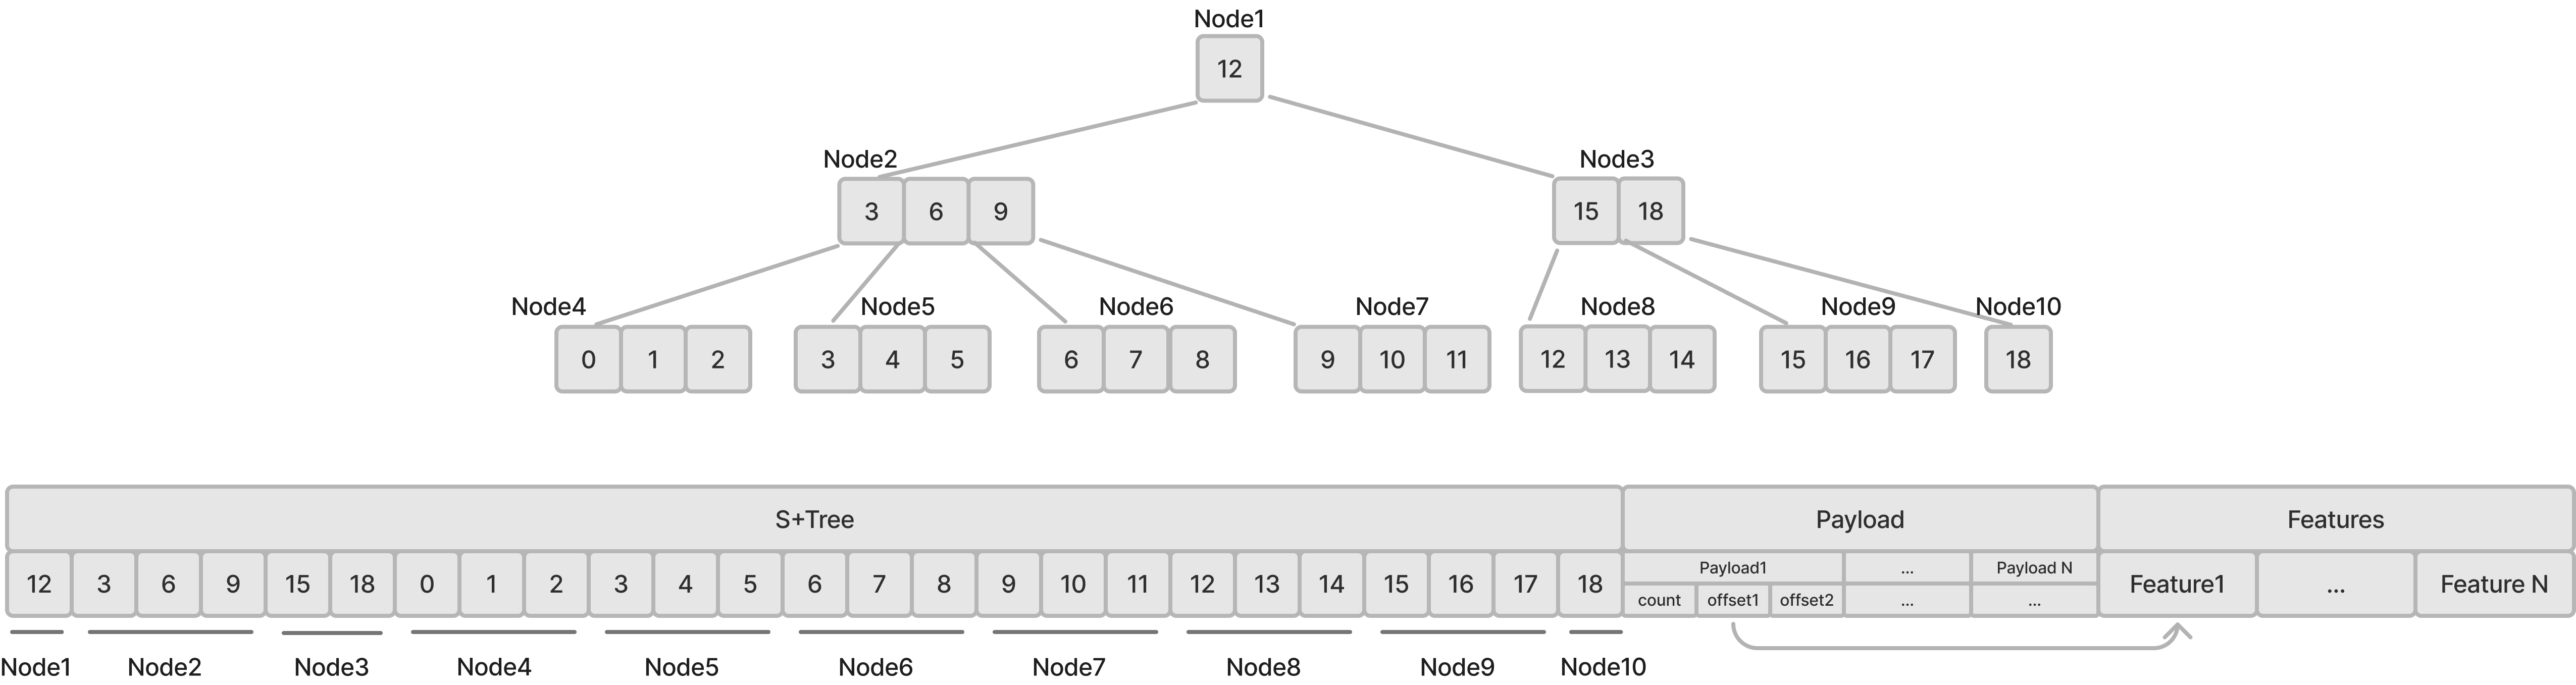
\includegraphics[width=0.8\textwidth]{figs/methodology/attribute_index.png}
  \caption{Attribute index implementation in FlatCityBuf}
  \label{fig:methodology:attribute_index}
\end{figure}

The B+tree structure is organized as follows:

\begin{itemize}
    \item \textbf{Internal Nodes}: Each internal node contains a sequence of key-pointer pairs, where keys are attribute values and pointers are byte offsets to child nodes. The number of pairs per node is determined by the branching factor.
    
    \item \textbf{Leaf Nodes}: Leaf nodes contain key-offset pairs, where keys are attribute values and offsets either point directly to features or to the payload section for duplicate keys.
    
    \item \textbf{Payload Section}: A contiguous area storing arrays of feature offsets for duplicate key values. Each array begins with a 32-bit count followed by the corresponding feature offsets.
\end{itemize}

The tree construction process begins by sorting the attribute values and their corresponding feature offsets. For attributes with duplicate values, a payload section is created to store multiple offsets. The tree is then built bottom-up, with internal nodes containing separator keys and pointers to child nodes.

The index is structured to optimize for HTTP Range Requests, with several techniques employed to minimize network overhead:

\begin{itemize}
    \item \textbf{Streaming search}: The search algorithm operates in a streaming fashion, requesting only the nodes necessary for query evaluation in sequential order. This approach ensures that even with large indices, the system avoids loading the entire tree structure into memory, significantly reducing resource requirements.
    \item \textbf{Payload Prefetching}: Proactively caches parts of the payload section during initial query execution, reducing HTTP requests for duplicate keys.
    \item \textbf{Batch Payload Resolution}: Collects multiple payload references during tree traversal and resolves them with consolidated HTTP requests.
    \item \textbf{Request Batching}: Groups adjacent node requests to minimise network roundtrips.
    \item \textbf{Block Alignment}: Nodes are aligned to 4KB boundaries to match typical file system and HTTP caching patterns.
\end{itemize}

During query execution, the system interprets the provided condition (\eg, \texttt{building\_height > 25}) and traverses the appropriate attribute index to find matching features. The search algorithm adapts based on the condition type, using different traversal strategies for exact matches versus range queries. Results are returned as a set of feature offsets, which can then be used to retrieve the actual feature data from the features section of the file.

\subsection{Type-Specific Serialisation}
\label{methodology:attribute_index:type_specific_serialisation}

The attribute index supports various data types common in 3D city models, including:

\begin{itemize}
    \item \textbf{Numeric Types}: Integers (i8, i16, i32, i64, u8, u16, u32, u64) and floating-point values (f32, f64)
    \item \textbf{Temporal Types}: Dates and timestamps with timezone information
    \item \textbf{String Types}: Fixed-width strings with prefix encoding
    \item \textbf{Boolean Values}: Represented as single bytes
\end{itemize}

Each type implements a specialised serialisation strategy that preserves ordering semantics while optimising storage efficiency. For floating-point values, the implementation uses `OrderedFloat` to handle NaN values correctly. Strings utilise a fixed-width prefix encoding that balances storage requirements with efficient comparison operations.

\subsection{Duplicate Key Handling}
\label{methodology:attribute_index:duplicate_key_handling}

A significant optimisation in the attribute index is the handling of duplicate keys:

\begin{itemize}
    \item \textbf{Primary Index Structure}: Contains only unique keys, with pointers to either direct feature offsets or to a payload section
    \item \textbf{Payload Section}: Stores lists of offsets for duplicate key values
    \item \textbf{Tag Bit}: The most significant bit of the offset value indicates whether it points directly to a feature or to the payload section
\end{itemize}

This approach maintains the efficiency of the tree structure while properly handling attributes with many duplicate values. For example, building type attributes often have many identical values (e.g., hundreds of "residential" buildings), which are all efficiently indexed through a single payload reference.

\subsection{Query strategies}
\label{methodology:attribute_index:query_strategies}

The implementation contains two primary functions to achieve the goal of efficient query execution:

\begin{itemize}
    \item \textbf{find\_exact\_match}: The search algorithm traverses the tree to find the exact match for the given key.
    \item \textbf{find\_partition\_point}: The search algorithm traverses the tree to find the partition points for the given query value.
\end{itemize}

With these two functions, the implementation can handle both exact match and range queries. Range queries are implemented by finding the lower and upper bounds with using \texttt{find\_partition\_point} and then traversing the tree to collect the results.

% \subsection{Multi-Index Query Execution}
% \label{methodology:attribute_index:multi_index_query}

% The attribute indexing system supports complex queries across multiple attributes through a coordinated query execution strategy:

% \begin{enumerate}
%     \item Each condition in the query is evaluated against the appropriate attribute index
%     \item Results from individual conditions are represented as sets of feature offsets
%     \item For conjunctive queries (AND logic), set intersection determines the final result
%     \item For disjunctive queries (OR logic), set union combines the results
% \end{enumerate}

% The implementation provides specialised index structures for different access patterns:

% \begin{itemize}
%     \item \textbf{MemoryIndex}: For in-memory operations with the entire index loaded
%     \item \textbf{StreamIndex}: For file-based access using standard Read+Seek operations
%     \item \textbf{HttpIndex}: For remote access using HTTP Range Requests
% \end{itemize}

% Each implementation provides semantically equivalent operations while optimising for its specific access pattern, ensuring consistent results regardless of the access method.


%!TEX root = ../../thesis.tex

\section{Feature Encoding}
\label{methodology:feature_encoding}

The feature encoding section of FlatCityBuf is responsible for the binary representation of 3D city objects and their associated data. This component preserves the semantic richness of the CityJSON model while leveraging FlatBuffers' efficient binary serialisation. The full schema definition for feature encoding can be found in \autoref{appendix:flatcitybuf_schema:feature}.

\subsection{CityFeature and CityObject Structure}
\label{methodology:feature_encoding:cityfeature_cityobject_structure}

FlatCityBuf implements the core structure of \ac{cjseq} using the following FlatBuffers tables:

\begin{itemize}
  \item \textbf{CityFeature} - \textit{table (root object)} - The top-level container for city objects:
    \begin{itemize}
      \item \textit{id} - Required string identifier, marked as a key field for fast lookup
      \item \textit{objects} - Array of CityObject tables representing individual 3D features
      \item \textit{vertices} - Array of Vertex structs containing quantized X,Y,Z coordinates (int32)
      \item \textit{appearance} - Optional Appearance table with visual styling information
    \end{itemize}

  \item \textbf{CityObject} - \textit{table} - Individual 3D city objects:
    \begin{itemize}
      \item \textit{type} - CityObjectType enum (Building, Bridge, etc.) following CityJSON types \citep{cityjson_spec}
      \item \textit{id} - Required string identifier, marked as a key field
      \item \textit{geographical\_extent} - 3D bounding box as GeographicalExtent struct
      \item \textit{geometry} - Array of Geometry tables containing shape information
      \item \textit{attributes} - Binary blob containing attribute values (interpretable via columns schema)
      \item \textit{columns} - Array of Column tables defining attribute schema
      \item \textit{children} - Array of string IDs referencing child objects
      \item \textit{children\_roles} - Array of strings describing relationship roles
      \item \textit{parents} - Array of string IDs referencing parent objects
      \item \textit{extension\_type} - Optional string for extended object types (e.g., "+NoiseBuilding")
    \end{itemize}
\end{itemize}

This structure maintains CityJSON's hierarchical organization while taking advantage of FlatBuffers' binary encoding and zero-copy access capabilities. The one-to-many relationship between CityFeatures and CityObjects enables efficient vertex sharing while preserving semantic distinctions between different city elements.

\subsection{Geometry Encoding}
\label{methodology:feature_encoding:geometry_encoding}

Geometry in FlatCityBuf follows CityJSON's boundary representation (B-rep) model with flattened arrays for FlatBuffers encoding:

\begin{itemize}
  \item \textbf{Geometry} - \textit{table} - Container for geometric representation:
    \begin{itemize}
      \item \textit{type} - GeometryType enum representing dimensions (0D-Point, 1D-LineString, etc.)
      \item \textit{lod} - Level of Detail as float value
      \item \textit{boundaries} - Array of 32-bit indices referencing vertices
      \item \textit{strings} - Array of counts defining vertex groups
      \item \textit{surfaces} - Array of counts defining string groups
      \item \textit{shells} - Array of counts defining surface groups
      \item \textit{solids} - Array of counts defining shell groups
      \item \textit{semantics\_boundaries} - Parallel arrays to boundaries for semantic classification
      \item \textit{semantics\_values} - Array of SemanticObject tables
    \end{itemize}

  \item \textbf{SemanticObject} - \textit{table} - Semantic classification of geometry parts:
    \begin{itemize}
      \item \textit{type} - SemanticSurfaceType enum (WallSurface, RoofSurface, etc.)
      \item \textit{extension\_type} - Optional string for extended semantic types
      \item \textit{attributes} - Binary blob containing semantic-specific attributes
      \item \textit{columns} - Array of Column tables defining attribute schema
      \item \textit{parent} - Index to parent semantic object
      \item \textit{children} - Array of indices to child semantic objects
    \end{itemize}

  \item \textbf{GeometryInstance} - \textit{table} - Reference to template geometry:
    \begin{itemize}
      \item \textit{transformation} - 4×4 transformation matrix as TransformationMatrix struct
      \item \textit{template} - Index referencing a template in the header section
      \item \textit{boundaries} - Single-element array containing reference point index
    \end{itemize}

  \item \textbf{Vertex} - \textit{struct} - Quantized 3D coordinates:
    \begin{itemize}
      \item \textit{x, y, z} - Integer coordinates, converted to global coordinates using header transform
    \end{itemize}
\end{itemize}

\subsubsection{Hierarchical Boundaries as Flattened Arrays}
\label{methodology:feature_encoding:geometry_encoding:flattened_arrays}

A key challenge in adapting CityJSON's recursive boundary representation to FlatBuffers is that FlatBuffers does not support nested arrays. FlatCityBuf addresses this by implementing a dimensional hierarchy encoded as parallel flattened arrays:

\begin{figure}[h]
  \centering
  \todo{add figure}
  % \includegraphics[width=0.8\textwidth]{figs/methodology/boundary_encoding.png}
  \caption{Hierarchical encoding of boundary representation using flattened arrays}
  \label{fig:methodology:boundary_encoding}
\end{figure}

The encoding strategy follows a dimensional hierarchy from lowest to highest dimension:

\begin{enumerate}
  \item \textbf{boundaries}: A single flattened array of integer vertex indices
  \item \textbf{strings}: Array where each value indicates the number of vertices in each ring/boundary
  \item \textbf{surfaces}: Array where each value indicates the number of strings/rings in each surface
  \item \textbf{shells}: Array where each value indicates the number of surfaces in each shell
  \item \textbf{solids}: Array where each value indicates the number of shells in each solid
\end{enumerate}

For example, a simple triangle would be encoded as:

\begin{verbatim}
boundaries: [0, 1, 2]       // Indices of three vertices
strings: [3]                // Single string with 3 vertices
surfaces: [1]               // Single surface containing 1 string
\end{verbatim}

A more complex structure such as a cube (a solid with 6 quadrilateral faces) would be encoded as:

\begin{verbatim}
boundaries: [0, 1, 2, 3, 0, 3, 7, 4, 1, 5, 6, 2, 4, 7, 6, 5, 0, 4, 5, 1, 2, 6, 7, 3]
strings: [4, 4, 4, 4, 4, 4]    // 6 strings with 4 vertices each
surfaces: [1, 1, 1, 1, 1, 1]   // 6 surfaces with 1 string each
shells: [6]                    // 1 shell with 6 surfaces
solids: [1]                    // 1 solid with 1 shell
\end{verbatim}

\subsubsection{Semantic Surface Encoding}
\label{methodology:feature_encoding:geometry_encoding:semantics}

Semantic surface information is encoded using a similar approach:

\begin{itemize}
  \item \textbf{semantics\_values}: Array of SemanticObject tables containing type classifications, attributes, and hierarchical relationships
  \item \textbf{semantics\_boundaries}: Array of indices that reference entries in semantics\_values, with a parallel structure to the geometry boundaries
\end{itemize}

This parallel structure allows each geometric component to have associated semantic information without requiring deeply nested structures. For example, in a building model where each face has a semantic classification (wall, roof, etc.), the semantics\_boundaries array would have the same structure as the boundaries array, with each surface having a corresponding semantic value.

Through this flattened array approach, FlatCityBuf preserves the rich hierarchical structure of CityJSON geometries while conforming to FlatBuffers' efficiency-oriented constraints on data organization.

\subsubsection{Geometry Template Encoding}
\label{methodology:feature_encoding:geometry_encoding:templates}

FlatCityBuf implements CityJSON's template mechanism for efficient representation of repeated geometry patterns, a common requirement in urban environments where many buildings, street furniture items, or other objects share identical geometric structures. The template approach separates the geometry definition from its instantiation:

\begin{itemize}
  \item \textbf{Template Definition}: Templates are defined once in the header section as full Geometry objects:
    \begin{itemize}
      \item Templates use the same Geometry table format described previously for standard geometries
      \item Template vertices are stored with double-precision coordinates (\texttt{DoubleVertex}) to maintain accuracy in the local coordinate system
      \item All template vertices for all templates are stored in a single flat array (\texttt{templates\_vertices})
      \item Indices within template boundaries reference positions in this dedicated template vertex array
    \end{itemize}

  \item \textbf{Template Instantiation}: CityObjects reference templates through GeometryInstance tables:
    \begin{itemize}
      \item \texttt{template}: A single unsigned integer index referencing a specific template in the header
      \item \texttt{boundaries}: Contains exactly one index referencing a vertex in the feature's vertex array, which serves as the reference point for placement
      \item \texttt{transformation}: A 4×4 transformation matrix (rotation, translation, scaling) that positions the template relative to the reference point
    \end{itemize}
\end{itemize}

This approach provides significant storage efficiency, as potentially complex geometries with hundreds or thousands of vertices can be represented using just a few bytes per instance. For example, a dataset with 1,000 identical street lamps would store the detailed lamp geometry once in the header, with each instance requiring only an index reference, reference point, and transformation matrix—typically less than 140 bytes per instance instead of potentially kilobytes of repeated geometry data.

The transformation matrix enables not only positioning but also scaling and rotation, allowing templates to be adapted to specific contexts. This is particularly valuable for features like trees, street furniture, or modular building components that maintain the same basic shape but may vary in size or orientation.

\subsection{Materials and Textures}
\label{methodology:feature_encoding:materials_textures}

FlatCityBuf supports CityJSON's appearance model through the following structures:

\begin{itemize}
  \item \textbf{Appearance} - \textit{table} - Container for visual styling information:
    \begin{itemize}
      \item \textit{materials} - Array of Material tables
      \item \textit{textures} - Array of Texture tables
      \item \textit{vertices\_texture} - Array of Vec2 structs for UV coordinates
      \item \textit{material\_mapping} - Array of MaterialMapping tables
      \item \textit{texture\_mapping} - Array of TextureMapping tables
      \item \textit{default\_theme\_material} - String identifying default material theme
      \item \textit{default\_theme\_texture} - String identifying default texture theme
    \end{itemize}

  \item \textbf{Material} - \textit{table} - Surface visual properties:
    \begin{itemize}
      \item \textit{name} - Required string identifier
      \item \textit{ambient\_intensity} - Double value from 0.0 to 1.0
      \item \textit{diffuse\_color} - Array of double values (RGB)
      \item \textit{emissive\_color} - Array of double values (RGB)
      \item \textit{specular\_color} - Array of double values (RGB)
      \item \textit{shininess} - Double value from 0.0 to 128.0
      \item \textit{transparency} - Double value from 0.0 to 1.0
      \item \textit{is\_smooth} - Boolean flag for smooth shading
    \end{itemize}

  \item \textbf{Texture} - \textit{table} - Image mapping information:
    \begin{itemize}
      \item \textit{type} - TextureFormat enum (PNG, JPG)
      \item \textit{image} - Required string containing image file name or URL
      \item \textit{wrap\_mode} - WrapMode enum (None, Wrap, Mirror, Clamp, Border)
      \item \textit{texture\_type} - TextureType enum (Unknown, Specific, Typical)
      \item \textit{border\_color} - Array of double values (RGBA)
    \end{itemize}

  \item \textbf{MaterialMapping} and \textbf{TextureMapping} - \textit{tables} - Link materials/textures to surfaces:
    \begin{itemize}
      \item \textit{theme} - String identifier for themes (e.g., "summer", "winter")
      \item \textit{values} - Indices to surfaces or boundaries
      \item \textit{material/texture} - Index to the referenced material or texture
    \end{itemize}
\end{itemize}

This implementation prioritizes efficient storage by referencing external texture files rather than embedding image data directly, enabling selective loading based on application requirements while maintaining full compatibility with CityJSON's appearance model.

\subsubsection{Texture Storage Design Rationale}
\label{methodology:feature_encoding:textures:rationale}

FlatCityBuf stores texture references rather than embedding texture data directly for several strategic reasons:

\begin{itemize}
  \item \textbf{Performance Priority}: Enables rapid loading of geometric and semantic data without the overhead of large texture files when not required.

  \item \textbf{On-demand Loading}: Supports selective texture loading based on application needs, beneficial for analysis-focused use cases.

  \item \textbf{Size Management}: Maintains reasonable file sizes for large-scale datasets, essential for spatial indexing operations.

  \item \textbf{Web Efficiency}: Aligns with HTTP caching mechanisms, optimizing repeated access in browser environments.
\end{itemize}

This approach follows established patterns in formats like glTF and I3S, prioritizing operational efficiency over self-contained packaging for city-scale datasets.

\subsection{Attribute Encoding}
\label{methodology:feature_encoding:attribute_encoding}

Attributes in FlatCityBuf are encoded as binary data with a schema defined through Column tables, which were detailed previously in \autoref{methodology:header:schema_indexing}. Rather than repeating column structure information, this section focuses on the binary encoding strategy:

\begin{itemize}
  \item \textbf{Attribute Binary Encoding} - Efficient type-specific serialization:
    \begin{itemize}
      \item \textit{Numeric types} - Native binary representation (little-endian)
      \item \textit{String} - Length-prefixed UTF-8 encoding
      \item \textit{Boolean} - Single byte (0 = false, 1 = true)
      \item \textit{Date/DateTime} - Standardized binary format
      \item \textit{Null} - Represented according to type (0, empty string, etc.)
    \end{itemize}
\end{itemize}

By encoding attributes as type-specific binary values with a corresponding schema, FlatCityBuf achieves significant storage efficiency compared to self-describing formats like JSON. The column-based approach also aligns with common database practices, facilitating integration with existing GIS and database systems. The figure below highlights the binary encoding process for different attribute types, demonstrating how the schema-driven approach reduces storage requirements while maintaining full data fidelity.

\todo{add figure}
\begin{figure}[h]
  \centering
  % \includegraphics[width=0.8\textwidth]{figures/attribute_encoding.png}
  \caption{Attribute Encoding Process}
  \label{methodology:feature_encoding:attribute_encoding:figure}
\end{figure}

\subsection{Extension Mechanism}
\label{methodology:feature_encoding:extension_mechanism}

FlatCityBuf provides comprehensive support for CityJSON's extension mechanism, which was previously detailed in \autoref{methodology:header:extensions}. While the extension structures are defined in the header, their implementation within actual city features requires specific encoding strategies that balance extensibility with performance.

\subsubsection{Encoding of Extended City Objects}
\label{methodology:feature_encoding:extension_mechanism:city_objects}

Extended city object types (those prefixed with "+") are encoded using a two-part strategy:

\begin{itemize}
  \item A standard enum value \texttt{ExtensionObject} is used for the \texttt{type} field, providing efficient storage and processing
  \item The actual extension type name (e.g., "+NoiseCityFurnitureSegment") is stored in the \texttt{extension\_type} string field
\end{itemize}

This hybrid approach offers an optimal balance: the fixed enum value enables fast processing and type checking, while the string field preserves the full semantic information without requiring enum updates for new extension types.

\subsubsection{Encoding of Extended Semantic Surfaces}
\label{methodology:feature_encoding:extension_mechanism:semantic_surfaces}

Similarly, extended semantic surface types follow the same pattern:

\begin{itemize}
  \item The \texttt{type} field uses the enum value \texttt{ExtraSemanticSurface}
  \item The specific type (e.g., "+ThermalSurface") is stored in the \texttt{extension\_type} field
\end{itemize}

\subsubsection{Extension Attribute Encoding}
\label{methodology:feature_encoding:extension_mechanism:attributes}

Extension-specific attributes are encoded using the same binary serialization mechanism as core attributes:

\begin{itemize}
  \item Extension attributes are included in the same binary attribute blob as standard attributes
  \item The schema for these attributes is derived from the extension definition in the header
  \item No distinction is made at the storage level between core and extension attributes, simplifying implementation
\end{itemize}

During decoding:
\begin{itemize}
  \item If a CityObject has \texttt{type=ExtensionObject}, the application uses \texttt{extension\_type} to determine proper handling
  \item All attributes are decoded according to the provided schema, regardless of whether they belong to the core CityJSON specification or to an extension
\end{itemize}

Unlike CityJSON, which references external schema files for extensions, FlatCityBuf's self-contained approach ensures that all extension information is available within a single file. This approach maintains the cloud-optimized philosophy of minimizing external dependencies while preserving full compatibility with the rich extension capabilities of CityJSON.


%!TEX root = ../../thesis.tex

\section{HTTP Range Requests and Cloud Optimisation}
\label{methodology:http_range_requests}

A critical component of cloud-optimised geospatial formats is their ability to support selective data retrieval without downloading entire datasets. FlatCityBuf achieves this capability through strategic implementation of HTTP Range Requests, enabling efficient web-based access to 3D city models. This section details the technical implementation, optimisation strategies, and cross-platform compatibility of this mechanism.

\subsection{Principles of Partial Data Retrieval}
\label{methodology:http_range_requests:partial_retrieval_principles}

HTTP Range Requests, defined in RFC 7233, allow clients to request specific byte ranges from server resources instead of entire files. FlatCityBuf's structure is specifically designed to leverage this capability, with particular attention to:

\begin{itemize}
    \item \textbf{Aligned Section Boundaries}: File sections are aligned to facilitate efficient range requests
    \item \textbf{Decoupled Components}: Header, indices, and features can be accessed independently
    \item \textbf{Index-Driven Retrieval}: Spatial and attribute indices determine which feature ranges to request
    \item \textbf{Request Minimisation}: Algorithms optimise for reducing the number of HTTP requests
\end{itemize}

The format's hierarchical indexing enables clients to perform sophisticated spatial and attribute queries while transferring only the minimal amount of data required, a critical factor for large-scale 3D city models that can exceed several gigabytes in size.

\subsection{Range Request Workflow}
\label{methodology:http_range_requests:range_request_workflow}

The HTTP Range Request workflow in FlatCityBuf follows a sequential process optimised for minimising network traffic:

\begin{enumerate}
    \item \textbf{Header Retrieval}: The client requests the magic bytes (4 bytes) and header size (4 bytes), followed by the complete header section. This provides essential metadata including coordinate reference systems, transformations, and index structure information.

    \item \textbf{Index Navigation}: Based on the query parameters (spatial bounding box or attribute conditions), the client navigates the appropriate index structures:
    \begin{itemize}
        \item For spatial queries, selective traversal of the R-tree requires retrieving only the nodes along the query path
        \item For attribute queries, traversal of the appropriate B+tree indices with similar selectivity
    \end{itemize}

    \item \textbf{Feature Resolution}: Using the byte offsets obtained from the indices, the client makes targeted range requests for specific features. The size of each feature is determined implicitly by the difference between consecutive offsets.

    \item \textbf{Progressive Processing}: Features are processed incrementally as they arrive, allowing applications to begin rendering or analysis before all data is received.
\end{enumerate}

This workflow achieves significant efficiency improvements over traditional approaches that require downloading entire datasets before processing can begin.

\subsection{Optimisation Techniques}
\label{methodology:http_range_requests:range_request_optimisations}

Network latency often dominates performance when accessing data over HTTP, with each request incurring significant overhead regardless of payload size. FlatCityBuf implements several techniques to minimise this overhead:

\begin{itemize}
    \item \textbf{Request Batching}: Adjacent feature requests are combined into single range requests when their proximity falls below a configurable threshold (typically 4KB). This significantly reduces the number of HTTP requests while avoiding excessive data transfer.

    \item \textbf{Prefetching Strategy}: The client proactively fetches portions of the index and payload sections based on statistical predictions of access patterns. For instance, the header retrieval also prefetches a small portion of the spatial index to optimise subsequent spatial queries.

    \item \textbf{Payload Prefetching}: For attribute indices with duplicate keys, a portion of the payload section (typically 16KB-1MB) is prefetched during initial query execution. This cache-first approach can eliminate up to 90\% of payload-related HTTP requests in typical workflows.

    \item \textbf{Buffered HTTP Client}: The implementation uses a buffered HTTP client that caches previously fetched data ranges, avoiding redundant requests when overlapping ranges are accessed.

    \item \textbf{Progressive Index Loading}: Only the portions of indices required for a specific query are loaded, rather than retrieving entire index structures.
\end{itemize}

These optimisations work in concert to minimise both the number of HTTP requests and the total data transferred, resulting in significantly improved performance for cloud-based 3D city model applications.

\subsection{Cross-Platform Implementation}
\label{methodology:http_range_requests:cross_platform_implementation}

FlatCityBuf provides range request capabilities across multiple platforms to maximise accessibility and integration options:

\subsubsection{Native Rust Implementation}
\label{methodology:http_range_requests:cross_platform_implementation:native_rust}

The primary implementation is a Rust library that provides:

\begin{itemize}
    \item \textbf{Async HTTP Client}: Non-blocking implementation using Rust's asynchronous I/O capabilities
    \item \textbf{Buffer Management}: Sophisticated caching of previously fetched ranges to minimise redundant requests
    \item \textbf{Query Optimisation}: Intelligent batching and request merging based on spatial and temporal locality
    \item \textbf{Streaming Interface}: Incremental processing through iterator-based APIs
\end{itemize}

This native implementation achieves optimal performance for server-side applications and desktop GIS tools.

\subsubsection{WebAssembly Module}
\label{methodology:http_range_requests:cross_platform_implementation:webassembly_module}

To support browser-based applications, FlatCityBuf includes a WebAssembly (WASM) module built from the same Rust codebase:

\begin{itemize}
    \item \textbf{JavaScript Interoperability}: Clean API for integration with web mapping libraries like Cesium and Mapbox
    \item \textbf{Fetch API Integration}: Uses the browser's native Fetch API with appropriate range headers
    \item \textbf{In-Browser Processing}: Performs index traversal and feature decoding directly in the browser
    \item \textbf{Memory-Efficient Design}: Implements streaming approaches to work within browser memory constraints
\end{itemize}

The WASM implementation currently has a limitation related to memory addressing. WebAssembly in browsers currently uses a 32-bit memory model, limiting addressable space to 4GB. While this is sufficient for most city-scale datasets, it can be a constraint for country-level models. The upcoming WebAssembly Memory64 proposal (currently at Stage 4 in the standardisation process) will eliminate this limitation by supporting 64-bit addressing.

\subsection{Performance Analysis}
\label{methodology:http_range_requests:performance_analysis}

Empirical testing with various datasets demonstrates the substantial performance benefits of HTTP Range Requests for FlatCityBuf:

\begin{itemize}
    \item \textbf{Data Transfer Reduction}: Spatial queries typically retrieve only 3-10\% of the total dataset size
    \item \textbf{Request Efficiency}: Optimisation techniques reduce HTTP requests by 80-95\% compared to naïve implementations
    \item \textbf{Latency Improvement}: Initial visualisation time improves by 10-20× compared to downloading complete datasets
    \item \textbf{Progressive Rendering}: Features appear incrementally, with first elements visible within milliseconds
\end{itemize}

These improvements are particularly pronounced for large datasets and bandwidth-constrained environments, enabling interactive 3D city model exploration even on mobile networks.

\subsection{Integration with Cloud Infrastructure}
\label{methodology:http_range_requests:cloud_integration}

The HTTP Range Request mechanism integrates seamlessly with modern cloud storage services:

\begin{itemize}
    \item \textbf{Static Hosting}: FlatCityBuf files can be served from standard object storage services like AWS S3, Google Cloud Storage, or Azure Blob Storage, all of which support range requests without additional server-side processing.

    \item \textbf{Content Delivery Networks}: The format works effectively with CDNs, which can cache range responses independently

    \item \textbf{CORS Configuration}: Cross-origin resource sharing headers allow browser-based clients to access remote datasets

    \item \textbf{Serverless Processing}: The client-side filtering approach eliminates the need for dedicated server-side processing
\end{itemize}

This infrastructure compatibility ensures that FlatCityBuf can be deployed in cost-effective cloud environments without requiring specialised server software or complex data pipelines.

\subsection{Real-World Applications}
\label{methodology:http_range_requests:real_world_applications}

The HTTP Range Request capabilities of FlatCityBuf enable several key application scenarios:

\begin{itemize}
    \item \textbf{Web-Based 3D Visualisation}: Browser applications can render specific city districts without downloading entire city models

    \item \textbf{Mobile Applications}: Resource-constrained devices can access only the data they need, reducing bandwidth usage and memory requirements

    \item \textbf{Distributed Analysis}: Cloud-based processing can extract specific features of interest for analysis without transferring complete datasets

    \item \textbf{Real-Time Updates}: New data can be appended to existing datasets and made immediately available through range requests
\end{itemize}

These application patterns demonstrate how the format's HTTP Range Request capabilities transform the accessibility and usability of large-scale 3D city models in cloud and web environments.


% Methodology-----------------------

\chapter{Result}
\label{chp:result}
\section{Overview}
\label{result:overview}
This chapter presents comprehensive evaluations of the FlatCityBuf format, demonstrating its performance characteristics and practical applicability through multiple assessment approaches. The evaluation encompasses both technical performance metrics and real-world implementation scenarios to provide a holistic understanding of the format's capabilities.

The chapter is structured around several key evaluation components. First, a web prototype implementation is presented to demonstrate FlatCityBuf's practical capabilities in browser environments, showcasing how the format enables partial data access for large 3D city models through HTTP Range Requests.

Second, the datasets used throughout the evaluation are described, including both the established benchmark datasets from \citet{ledoux_2024} and additional PLATEAU datasets from the Takeshiba district of Tokyo, providing context for the performance comparisons and ensuring reproducibility of results.

Third, file size comparisons are conducted across different encoding formats to evaluate storage efficiency and compression characteristics of FlatCityBuf relative to existing CityJSON variants.

Finally, web environment evaluations demonstrate real-world performance characteristics by measuring data retrieval times and network efficiency in browser-based scenarios. These tests specifically evaluate the effectiveness of HTTP Range Requests for selective data access, providing insights into bandwidth optimisation and response times critical for web-based 3D city model applications.

The following sections present detailed results from each evaluation component, culminating in integrated analyses that synthesise findings to provide comprehensive insights into FlatCityBuf's performance characteristics and practical benefits for 3D city model applications.

\subsection{Web Prototype}
\label{result:web_prototype}

\subsection{Cross-Platform Implementation}
\label{result:cross_platform_implementation}

FlatCityBuf provides range request capabilities across multiple platforms to maximise accessibility and integration options:
\subsubsection{Cross-Platform Support}
\label{result:cross_platform_implementation:cross_platform}

FlatCityBuf is implemented primarily as a Rust library that can be used in both native environments and web browsers. The same codebase is compiled to:

\begin{itemize}
  \item Native Rust library for server-side applications and desktop GIS tools
  \item \ac{wasm} module for browser-based applications with JavaScript interoperability
\end{itemize}

This cross-platform approach enables FlatCityBuf to work with both Rust's native HTTP clients and browser-based Fetch \ac{api} implementations. The \ac{wasm} implementation has one notable limitation: current browser \ac{wasm} implementations use a 32-bit memory model (4GB limit), which may constrain processing of country-level datasets. This limitation will be resolved with the upcoming \ac{wasm} Memory64 proposal \citep{WebAssemblyCoreSpecification2}.
\subsubsection{Web prototype}
\label{result:cross_platform_implementation:web_prototype}

To demonstrate FlatCityBuf's capabilities in web environments and illustrate practical user interactions with the data, a functional web prototype was developed. The prototype is publicly accessible at \url{https://fcb-web-prototype.netlify.app/}. It leverages the WebAssembly module of FlatCityBuf combined with TypeScript and React for the frontend implementation, with Cesium serving as the 3D map rendering engine.

The prototype operates on a substantial dataset covering approximately 20km $\times$ 20km of South Holland, Netherlands, stored as a single 3.4GB FlatCityBuf file. This file is delivered directly from Google Cloud Storage\citep{gcs}, a serverless storage service, where it exists as a static file similar to images or videos, requiring no specialized server-side processing. Despite this large file size, the application remains responsive by utilising the HTTP range request capabilities described in \autoref{result:cross_platform_implementation:cloud_integration}. Users can interact with the data through several query mechanisms:

\begin{itemize}
  \item \textbf{Spatial queries}: Users can filter features either by defining a spatial bounding box or by placing a point on the map to retrieve features based on intersection or nearest-neighbor relationships.

  \item \textbf{Attribute queries}: The interface supports filtering features through attribute conditions (\eg, \texttt{building id = 1, height > 10m}), demonstrating the attribute index capabilities.

  \item \textbf{Data export}: Users can download the filtered subset of features in CityJSONSeq format, showcasing the format conversion capabilities.
\end{itemize}

This prototype effectively demonstrates how FlatCityBuf enables browser-based applications to work with large 3D city models without downloading the entire dataset, providing responsive performance even on consumer-grade hardware and network connections.

\begin{figure}[ht]
  \centering
  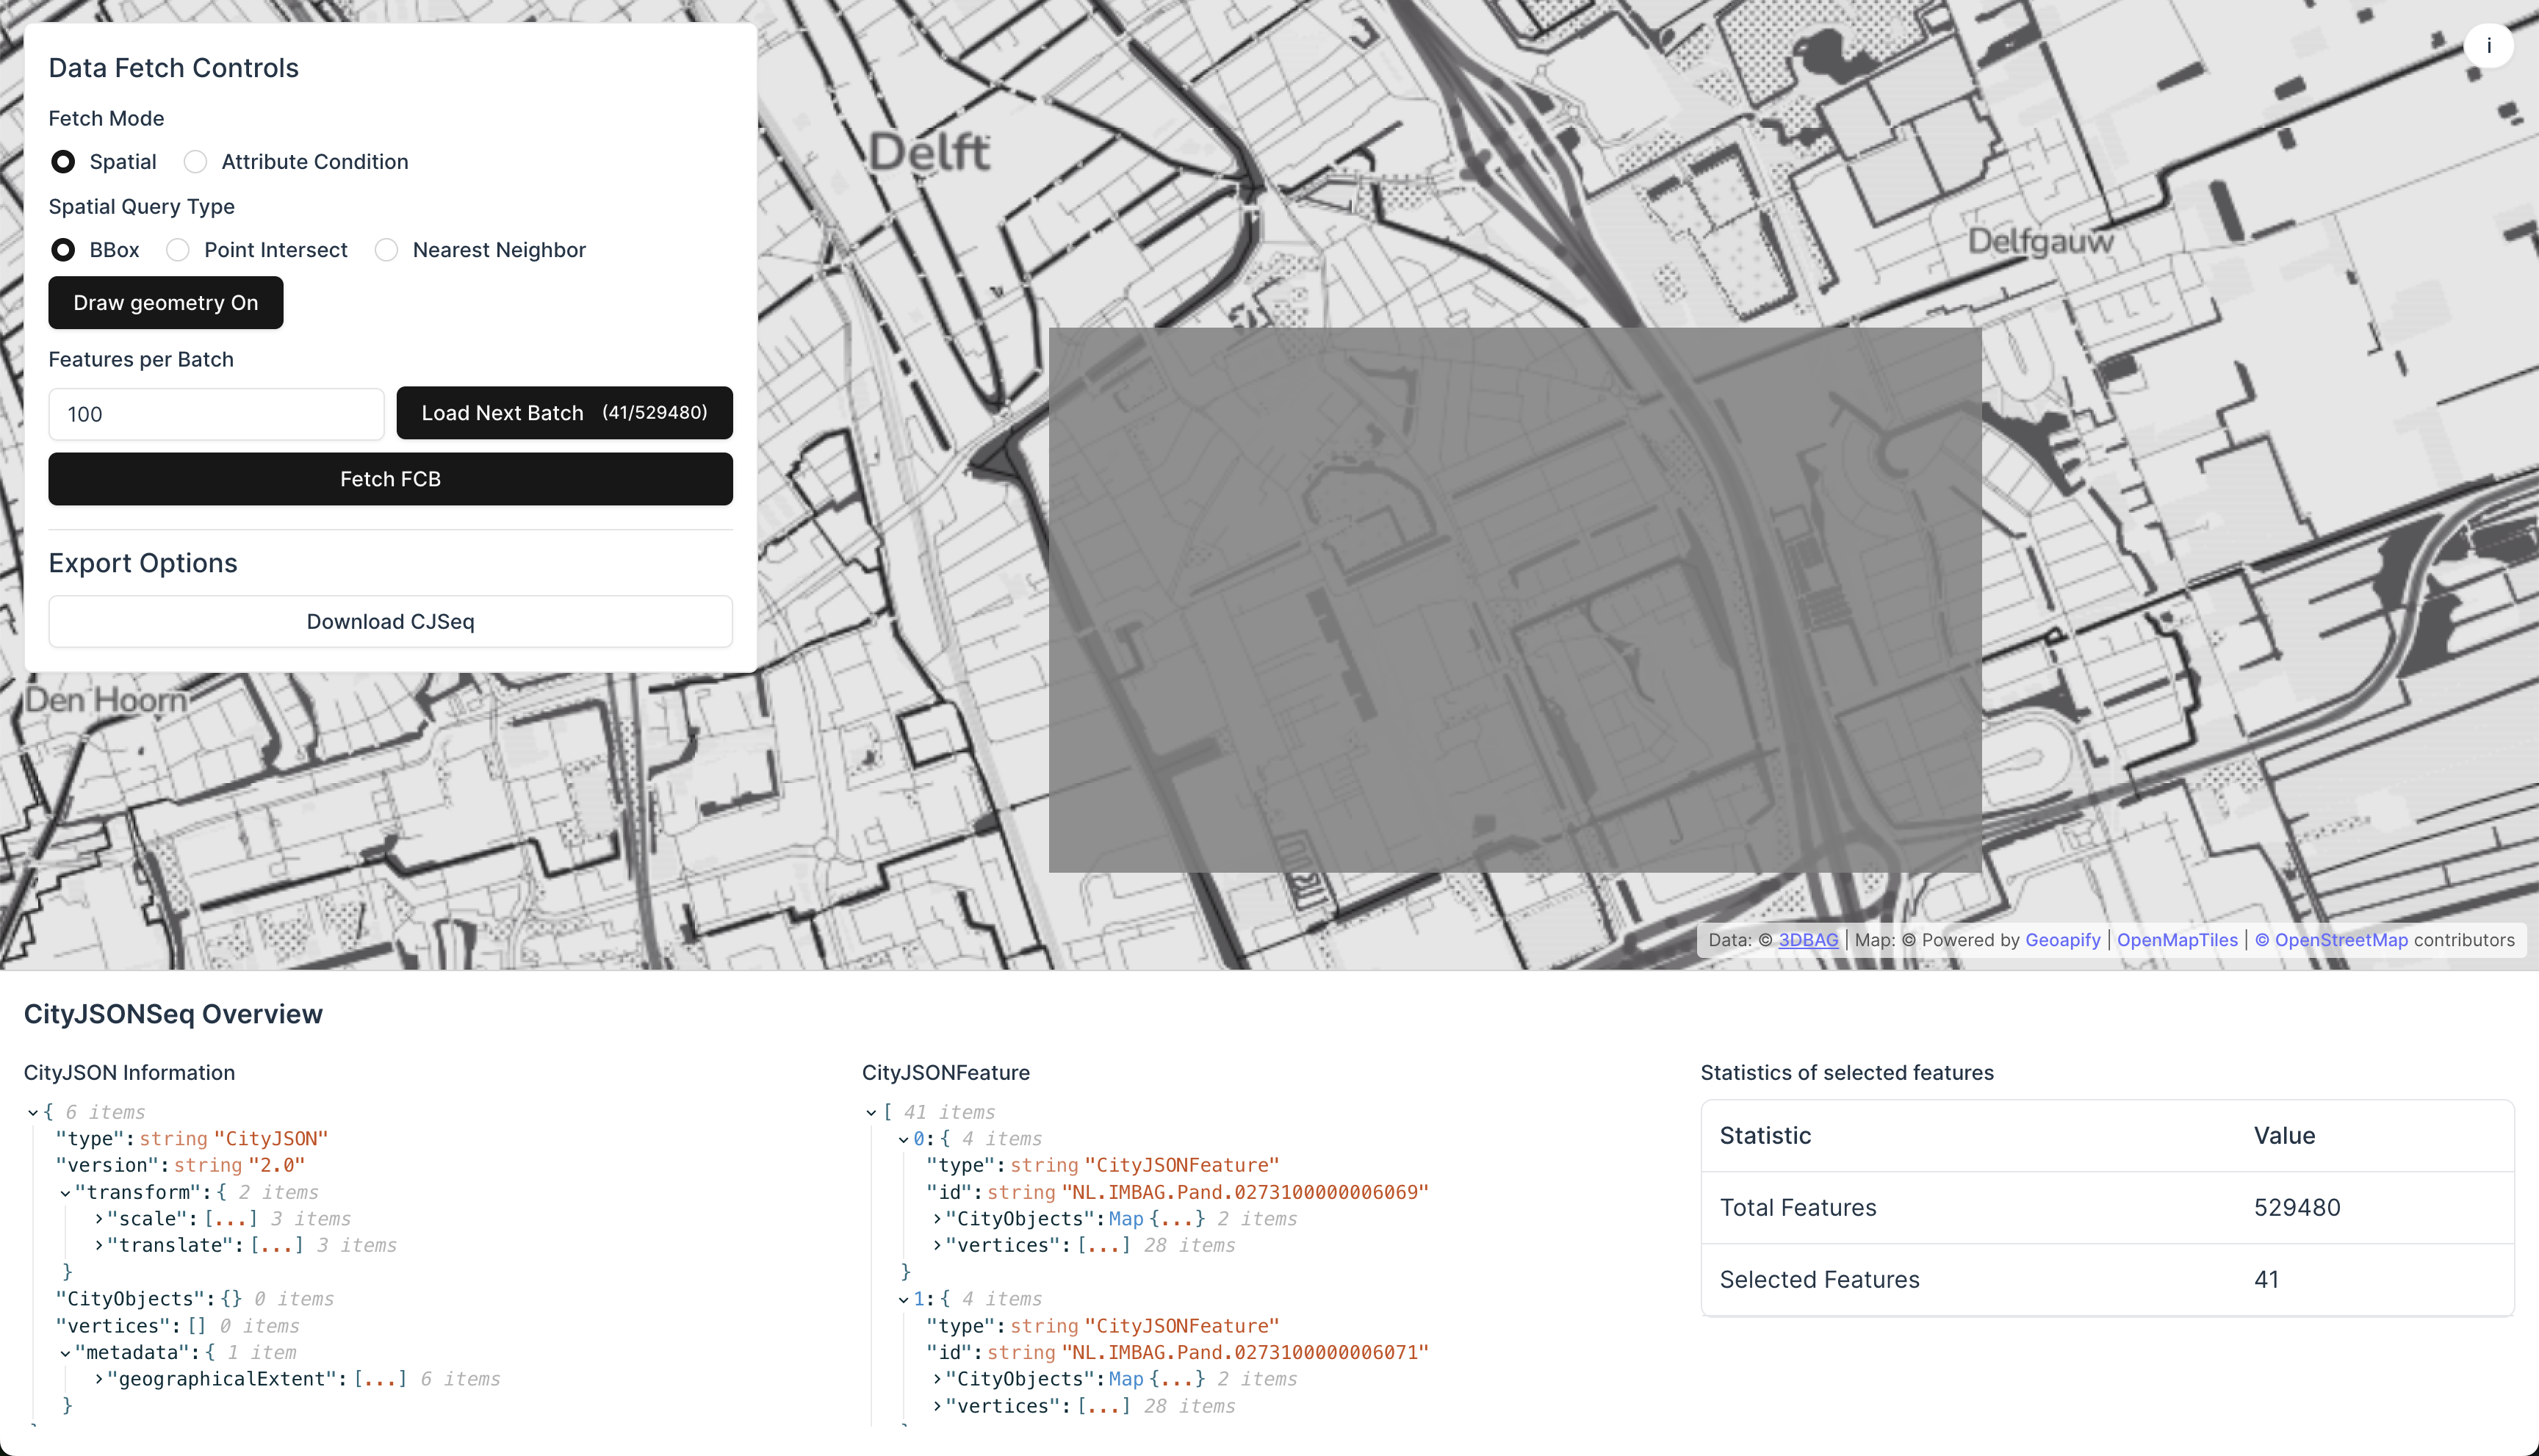
\includegraphics[width=1.0\textwidth]{figs/result_analysis/web_prototype.png}
  \caption{Web prototype of FlatCityBuf demonstrating spatial and attribute query capabilities on a 3.4GB dataset of South Holland.}
  \label{fig:result:cross_platform_implementation:web_prototype}
\end{figure}

\subsection{Integration with Cloud Infrastructure}
\label{result:cross_platform_implementation:cloud_integration}

The HTTP Range Request mechanism integrates seamlessly with modern cloud infrastructure. FlatCityBuf files can be served from standard object storage services like AWS S3, Google Cloud Storage, or Azure Blob Storage, all of which support range requests without additional server-side processing. This enables a serverless architecture where the client-side filtering approach eliminates the need for dedicated server-side processing. This infrastructure compatibility ensures that FlatCityBuf can be deployed in cost-effective cloud environments without requiring specialised application servers and databases.

\begin{figure}[ht]
  \centering
  \includegraphics[width=0.8\textwidth]{figs/result_analysis/server_architecture_fcb.png}
  \caption{Server architecture for FlatCityBuf. The client-side filtering approach eliminates the need for dedicated server-side processing.}
  \label{fig:result:cross_platform_implementation:server_architecture}
\end{figure}
\section{Datasets}
\label{result:dataset}

To evaluate file sizes and conduct both local and web-based benchmarks, we employed a diverse range of datasets from \citet{ledoux_2024} supplemented with additional datasets from PLATEAU \citep{plateau}. PLATEAU employs its own data specification combining CityGML 2.0 \citep{CityGML} with a custom \ac{ade}. The CityGML-encoded 3D city models were converted to CityJSON using citygml-tools, a command-line utility developed by \citet{citygml_tools}. Note that PLATEAU's \ac{ade} components are not included in the converted datasets since they are not compatible with the current CityJSON implementation.

To comprehensively evaluate FlatCityBuf, we utilised diverse PLATEAU models including buildings, bridges, transport, tunnels, and vegetation. The dataset collection spans various urban environments from small-scale architectural models to large metropolitan areas across European and Japanese cities, enabling evaluation across different feature types, geometric complexities, and data modeling approaches. \footnote{The datasets used in this evaluation are publicly available at \url{https://github.com/HideBa/flatcitybuf-data}.}

\section{File Size Comparison}
\label{result:file_size_comparison}

\subsection{File size results}
\label{result:overview:filesize_comparison}

\autoref{tab:dataset_comparison} presents a comparison of datasets in both CityJSONSeq and FlatCityBuf formats. The results demonstrate that FlatCityBuf encoding achieves superior compression for several datasets, including Helsinki, Ingolstadt, and New York City, with compression factors of 16.36\%, 19.09\%, and 20.17\% respectively. Conversely, the PLATEAU datasets exhibit the opposite trend, with CityJSONSeq format demonstrating better storage efficiency.
\begin{table*}
  \centering
  \begin{threeparttable}
    \caption{The datasets used for the benchmark.}
    \label{tab:dataset_comparison}
    \scriptsize
    \setlength{\tabcolsep}{1pt}
    \begin{tabular}{@{}lrrlrrr@{\hskip 2pt}rrrr@{}}
      \toprule
      & \multicolumn{3}{c}{\textbf{dataset}} & \multicolumn{3}{c}{\textbf{size of file}} & \multicolumn{4}{c}{\textbf{attributes}} \\
      \cmidrule(lr){2-4} \cmidrule(lr){5-7} \cmidrule(lr){8-11}
      & CityObj & CityFeat & app.$^{\text{(a)}}$ & CityJSONSeq & FlatCityBuf & compr.$^{\text{(b)}}$ & verts & avg$^{\text{(c)}}$ & obj$^{\text{(d)}}$ & sem$^{\text{(e)}}$ \\
      \midrule
      \textbf{3DBAG}          & 2221    & 1110   &      & \qty{5.87}{\mega\byte}  & \qty{6.23}{\mega\byte}  & $-6.02\%$  & 82612    & 74.43    & 37 & 1 \\
      \textbf{3DBV}           & 71634   & 71634  &      & \qty{317.34}{\mega\byte}& \qty{280.92}{\mega\byte}& $11.48\%$  & 4992893  & 69.70    & 64 & 0 \\
      \textbf{Helsinki}       & 77267   & 77231  &      & \qty{412.44}{\mega\byte}& \qty{344.96}{\mega\byte}& $16.36\%$  & 3039107  & 39.35    & 27 & 9 \\
      \textbf{Helsinki\_tex}  & 77267   & 77231  & tex  & \qty{643.70}{\mega\byte}& \qty{545.29}{\mega\byte}& $15.29\%$  & 3039107  & 39.35    & 28 & 9 \\
      \textbf{Ingolstadt}     & 379     & 55     &      & \qty{3.84}{\mega\byte}  & \qty{3.11}{\mega\byte}  & $19.09\%$  & 88001    & 1600.02  & 33 & 13 \\
      \textbf{Montréal}       & 294     & 294    & tex  & \qty{4.60}{\mega\byte}  & \qty{4.80}{\mega\byte}  & $-4.38\%$  & 32242    & 109.67   & 0  & 0 \\
      \textbf{NYC}            & 23777   & 23777  &      & \qty{95.45}{\mega\byte} & \qty{76.20}{\mega\byte} & $20.17\%$  & 1044145  & 43.91    & 3  & 3 \\
      \textbf{Rotterdam}      & 853     & 853    & tex  & \qty{2.69}{\mega\byte}  & \qty{2.80}{\mega\byte}  & $-3.98\%$  & 26679    & 31.28    & 5  & 0 \\
      \textbf{Vienna}         & 1322    & 307    &      & \qty{4.81}{\mega\byte}  & \qty{4.12}{\mega\byte}  & $14.32\%$  & 47229    & 153.84   & 7  & 4 \\
      \textbf{Zürich}         & 198699  & 52834  &      & \qty{247.12}{\mega\byte}& \qty{188.63}{\mega\byte}& $23.67\%$  & 3564542  & 67.47    & 8  & 0 \\
      \textbf{PLATEAU (Building)}  & 10405   & 4307   &      & \qty{76.94}{\mega\byte} & \qty{79.41}{\mega\byte} & $-3.22\%$  & 147754   & 34.31    & 14 & 2 \\
      \textbf{PLATEAU (Bridge)}  & 60      & 8      &      & \qty{4.78}{\mega\byte}  & \qty{5.21}{\mega\byte}  & $-9.09\%$  & 16357    & 2044.62  & 5  & 2 \\
      \textbf{PLATEAU (Railway)}   & 412     & 412    &      & \qty{4.15}{\mega\byte}  & \qty{4.23}{\mega\byte}  & $-1.90\%$  & 5846     & 14.19    & 3  & 2 \\
      \textbf{PLATEAU (Transport)}  & 8136    & 8136   &      & \qty{26.47}{\mega\byte} & \qty{26.62}{\mega\byte} & $-0.54\%$  & 45992    & 5.65     & 3  & 2 \\
      \textbf{PLATEAU (Tunnels)}   & 21      & 3      &      & \qty{4.86}{\mega\byte}  & \qty{4.64}{\mega\byte}  & $4.41\%$   & 12306    & 4102.00  & 4  & 1 \\
      \textbf{PLATEAU (Vegetation)}   & 936     & 936    &      & \qty{1.78}{\mega\byte}  & \qty{2.32}{\mega\byte}  & $-30.50\%$ & 2567     & 2.74     & 3  & 0 \\
      \bottomrule
    \end{tabular}
    \begin{tablenotes}[flushleft]
      \footnotesize
    \item[a] appearance: `tex' indicates textures are stored; `mat' indicates materials are stored
    \item[b] compression factor is $\frac{\text{CityJSONSeq} - \text{FlatCityBuf}}{\text{CityJSONSeq}}$ (positive values indicate size reduction)
    \item[c] average number of vertices per feature
    \item[d] number of attributes in city objects
    \item[e] number of semantic surface attributes in city objects
    \end{tablenotes}
  \end{threeparttable}
\end{table*}

\subsection{Analysis of file size results}
\label{result:overview:analysis_of_file_size_results}
Although \autoref{result:overview:filesize_comparison} provides a summary of file size comparisons, the factors influencing these outcomes require further investigation. This section analyses the underlying causes through controlled experiments with simplified datasets.

\subsubsection{Level of detail}
\label{result:overview:analysis_of_file_size_results:level_of_detail}

To examine how \ac{lod} affects file size, I conducted a series of tests using the TU Delft BK building model at various \ac{lod} levels. Each \ac{lod} variant was systematically extracted from the original model, with attributes and semantic information deliberately removed to isolate the effect of geometric complexity. \autoref{tab:lod_comparison} presents the results of this analysis.

Since each test dataset contains only a single city feature, we compare feature sizes rather than total file sizes. This approach is necessary because FlatCityBuf incorporates a larger header structure, which would disproportionately affect comparisons involving minimal features.

The results demonstrate that while file sizes increase with higher levels of detail, the compression factor remains largely independent of \ac{lod}. Both formats show similar proportional growth in size as geometric complexity increases, with FlatCityBuf consistently achieving approximately 24-25\% size reduction compared to CityJSONSeq regardless of the \ac{lod} level. This suggests that the compression efficiency is determined by the underlying format design rather than the geometric complexity of the data.

\begin{table}[htbp]
  \centering
  \caption{Comparison of file sizes across different levels of detail for the TU Delft BK building model.}
  \label{tab:lod_comparison}
  \begin{tabular}{@{}lrrrr@{}}
    \toprule
    \textbf{Dataset} & \textbf{FlatCityBuf}$^{\text{(a)}}$ & \textbf{CityJSONSeq}$^{\text{(b)}}$ & \textbf{Compression} & \textbf{Vertices} \\
    \midrule
    TUD BK All & \qty{139.75}{\kilo\byte} & \qty{189.01}{\kilo\byte} & $26.08\%$ & 4549 \\
    TUD BK \ac{lod}0 & \qty{12.77}{\kilo\byte} & \qty{20.72}{\kilo\byte} & $38.11\%$ & 785 \\
    TUD BK \ac{lod}1.2 & \qty{37.45}{\kilo\byte} & \qty{49.40}{\kilo\byte} & $24.23\%$ & 1350 \\
    TUD BK \ac{lod}1.3 & \qty{44.66}{\kilo\byte} & \qty{59.25}{\kilo\byte} & $24.67\%$ & 1600 \\
    TUD BK \ac{lod}2.2 & \qty{62.02} {\kilo\byte} & \qty{82.74}{\kilo\byte} & $25.07\%$ & 2168 \\
    \bottomrule
  \end{tabular}
  \begin{tablenotes}[flushleft]
    \footnotesize
  \item[a] Average feature size in bytes in FlatCityBuf: $\frac{\text{Total FlatCityBuf size}}{\text{Number of features}}$
  \item[b] Average feature size in bytes in CityJSONSeq: $\frac{\text{Total CityJSONSeq size}}{\text{Number of features}}$

  \end{tablenotes}
\end{table}

\subsubsection{Attributes}
\label{result:overview:analysis_of_file_size_results:attributes}

To assess the impact of attributes on file size, we tested simple cube models from \citep{cityjson_dataset} with varying numbers of attributes. We systematically generated random attributes for each test case, examining both integer and string data types to determine their effect on compression efficiency. \autoref{tab:attribute_comparison} presents the results of this analysis.

\begin{table}[htbp]
  \centering
  \caption{Comparison of file sizes with varying numbers of attributes for simple cube models.}
  \label{tab:attribute_comparison}
  \begin{tabular}{@{}lrrrr@{}}
    \toprule
    \textbf{Dataset} & \textbf{FlatCityBuf}$^{\text{(a)}}$ & \textbf{CityJSONSeq}$^{\text{(b)}}$ & \textbf{Compression}  \\
    \midrule
    10 attributes (int) & \qty{580}{\byte} & \qty{611}{\byte} & $5.07\%$ \\
    100 attributes (int) & \qty{1.62}{\kilo\byte} & \qty{2.44}{\kilo\byte} & $33.65\%$ \\
    1000 attributes (int) & \qty{12.17}{\kilo\byte} & \qty{21.78}{\kilo\byte} & $44.13\%$ \\
    10 attributes (string) & \qty{580}{\byte} & \qty{611}{\byte} & $5.07\%$ \\
    100 attributes (string) & \qty{1.62}{\kilo\byte} & \qty{2.44}{\kilo\byte} & $33.65\%$ \\
    1000 attributes (string) & \qty{12.17}{\kilo\byte} & \qty{21.78}{\kilo\byte} & $44.13\%$ \\
    \bottomrule
  \end{tabular}
  \begin{tablenotes}[flushleft]
    \footnotesize
  \item[a] Average feature size in bytes in FlatCityBuf: $\frac{\text{Total FlatCityBuf size}}{\text{Number of features}}$
  \item[b] Average feature size in bytes in CityJSONSeq: $\frac{\text{Total CityJSONSeq size}}{\text{Number of features}}$
  \end{tablenotes}
\end{table}

The randomly generated attributes in our test datasets followed a consistent pattern, as shown in the example below:

\begin{lstlisting}[caption={Example of a CityJSON feature with attributes},  basicstyle=\small]
{
  "type": "Building",
  "geometry": [...],
  "attributes": {
    "attr_1": "value_1",
    "attr_2": "value_2",
    "attr_3": "value_3",
    "attr_4": "value_4",
    "attr_5": "value_5",
    ...
    "attr_n": "value_n"
  }
}
\end{lstlisting}

For integer attribute tests, all values were randomly generated integers between 0 and 1000. For string attribute tests, values were randomly generated strings of varying lengths between 5 and 15 characters. This approach ensured a realistic representation of typical attribute data while maintaining controlled test conditions.

\begin{figure}[htbp]
  \centering
  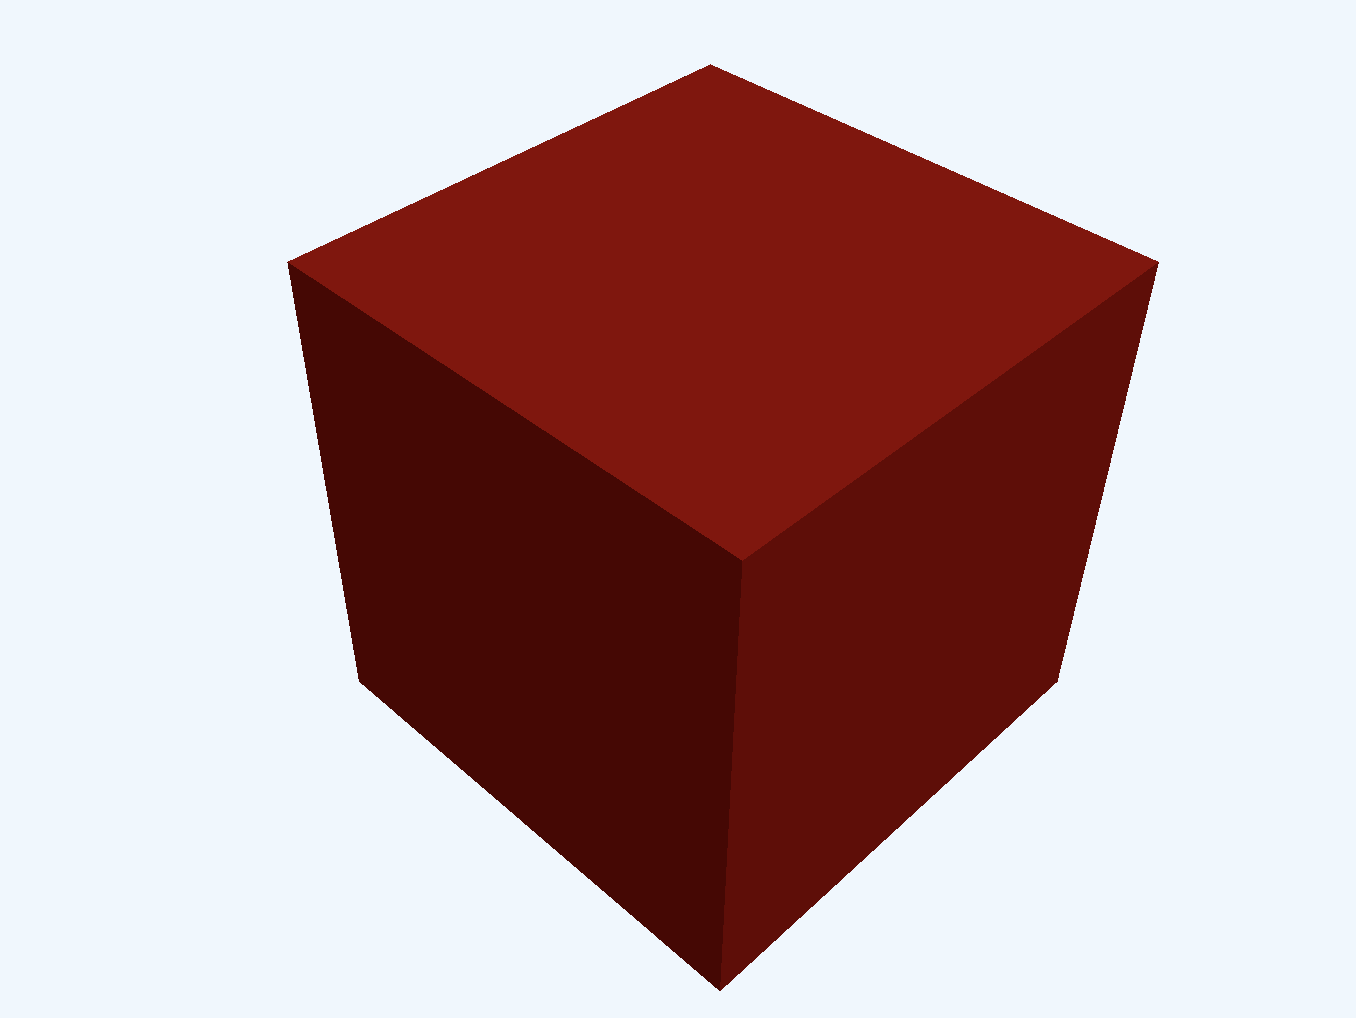
\includegraphics[width=0.48\textwidth]{figs/result_analysis/cube.png}
  \caption{Simple cube model used for attribute testing. This basic geometric structure provides a controlled environment for evaluating the impact of attributes on file size.}
  \label{fig:simple_cube}
\end{figure}

The results reveal a clear pattern: FlatCityBuf's compression advantage over CityJSONSeq increases substantially with the number of attributes. With only 10 attributes, the compression benefit is minimal at 5.07\%, but rises markedly to 33.65\% with 100 attributes and reaches 44.13\% with 1000 attributes.

This efficiency stems from FlatCityBuf's architectural design, which stores the attribute schema once in the file header. Each feature subsequently references attributes using only a 2-byte (u16) index, while CityJSONSeq must replicate identical attribute keys across all features. Although additional attributes increase the header size, this overhead is distributed across all features in the dataset. The header remains relatively compact—even with 1000 attributes, it occupies only a few tens of kilobytes.

These characteristics render FlatCityBuf particularly advantageous for datasets containing numerous attributes. The same efficiency applies to semantic surface attributes, where the schema-based approach provides similar compression benefits when features contain multiple surfaces with rich semantic information.

\subsubsection{Geometry complexity}
\label{result:overview:analysis_of_file_size_results:geometric_complexity}

To evaluate how geometric complexity influences file size, we analysed models with varying numbers of vertices. The test utilised two geometrically distinct models from the TU Delft campus dataset—one simple and one complex. To isolate the effect of geometry, attributes and semantic information were removed, leaving only the essential geometric components required by CityJSON. \autoref{tab:geometry_comparison} presents the numerical results of this analysis, while \autoref{fig:geometry_comparison} provides visual comparisons of the models.

\begin{table}[htbp]
  \centering
  \caption{Comparison of file sizes with varying geometric complexity.}
  \label{tab:geometry_comparison}
  \begin{tabular}{@{}lrrrr@{}}
    \toprule
    \textbf{Dataset} & \textbf{FlatCityBuf}$^{\text{(a)}}$ & \textbf{CityJSONSeq}$^{\text{(b)}}$ & \textbf{Compression} & \textbf{Vertices/Feature} \\
    \midrule
    TUD BK & \qty{139.75}{\kilo\byte} & \qty{189.01}{\kilo\byte} & $26.06\%$ & 4549 \\
    TUD Simple & \qty{13.12}{\kilo\byte} & \qty{15.42}{\kilo\byte} & $14.94\%$ & 340 \\
    \bottomrule
  \end{tabular}
  \begin{tablenotes}[flushleft]
    \footnotesize
  \item[a] Average feature size in bytes in FlatCityBuf: $\frac{\text{Total FlatCityBuf size}}{\text{Number of features}}$
  \item[b] Average feature size in bytes in CityJSONSeq: $\frac{\text{Total CityJSONSeq size}}{\text{Number of features}}$
  \end{tablenotes}
\end{table}

\begin{figure}[htbp]
  \centering
  \begin{subfigure}{0.48\textwidth}
    \centering
    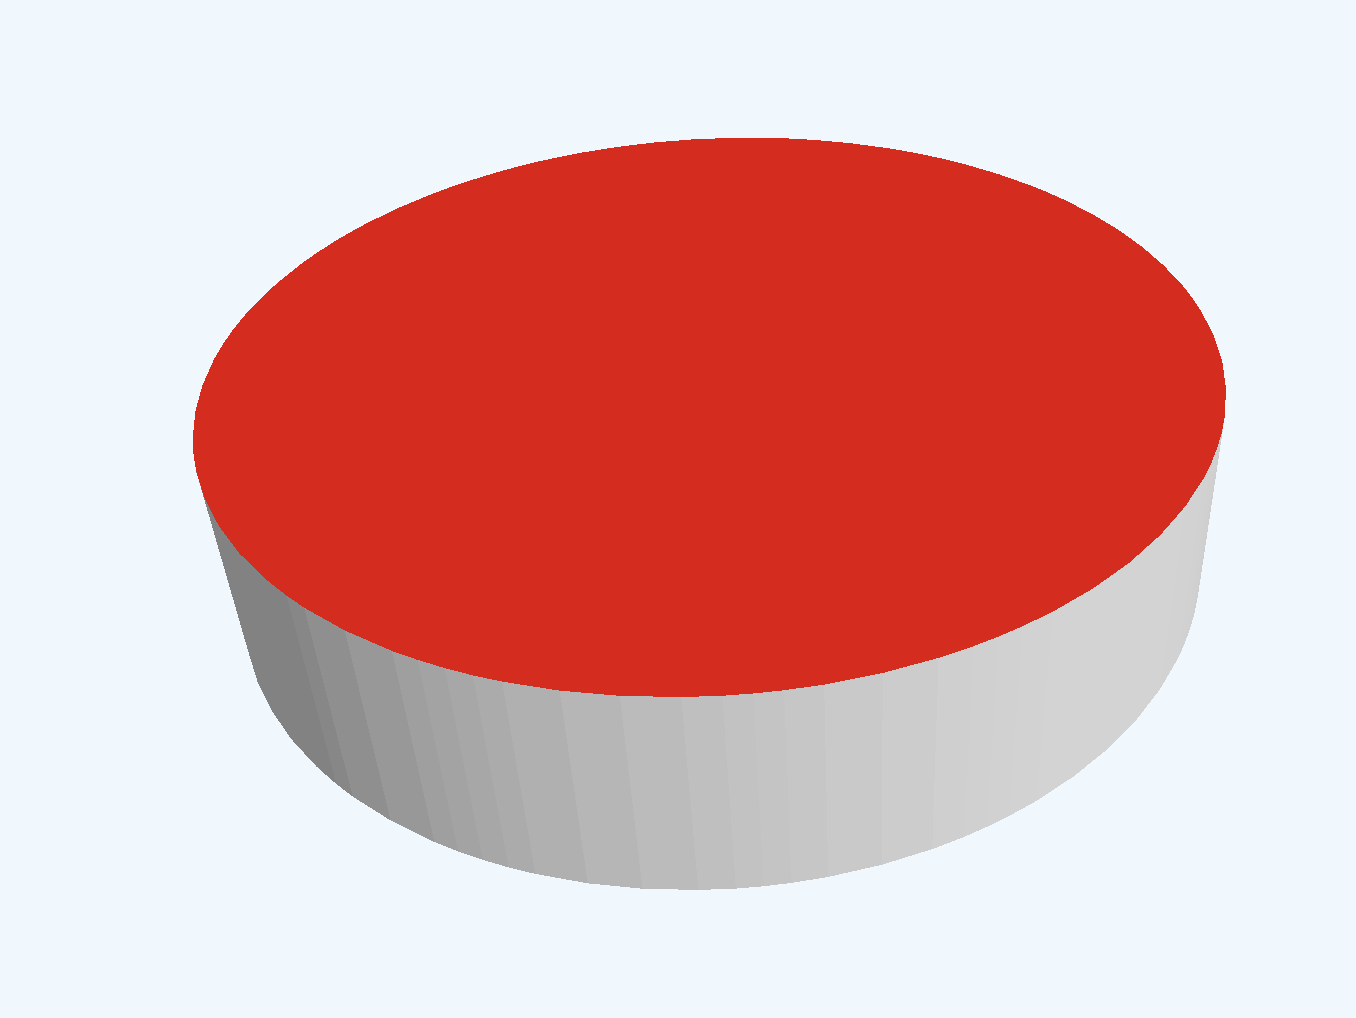
\includegraphics[width=\textwidth]{figs/result_analysis/tud_simple.png}
    \caption{TUD Simple model (340 vertices/feature)}
    \label{fig:tud_simple}
  \end{subfigure}
  \hfill
  \begin{subfigure}{0.48\textwidth}
    \centering
    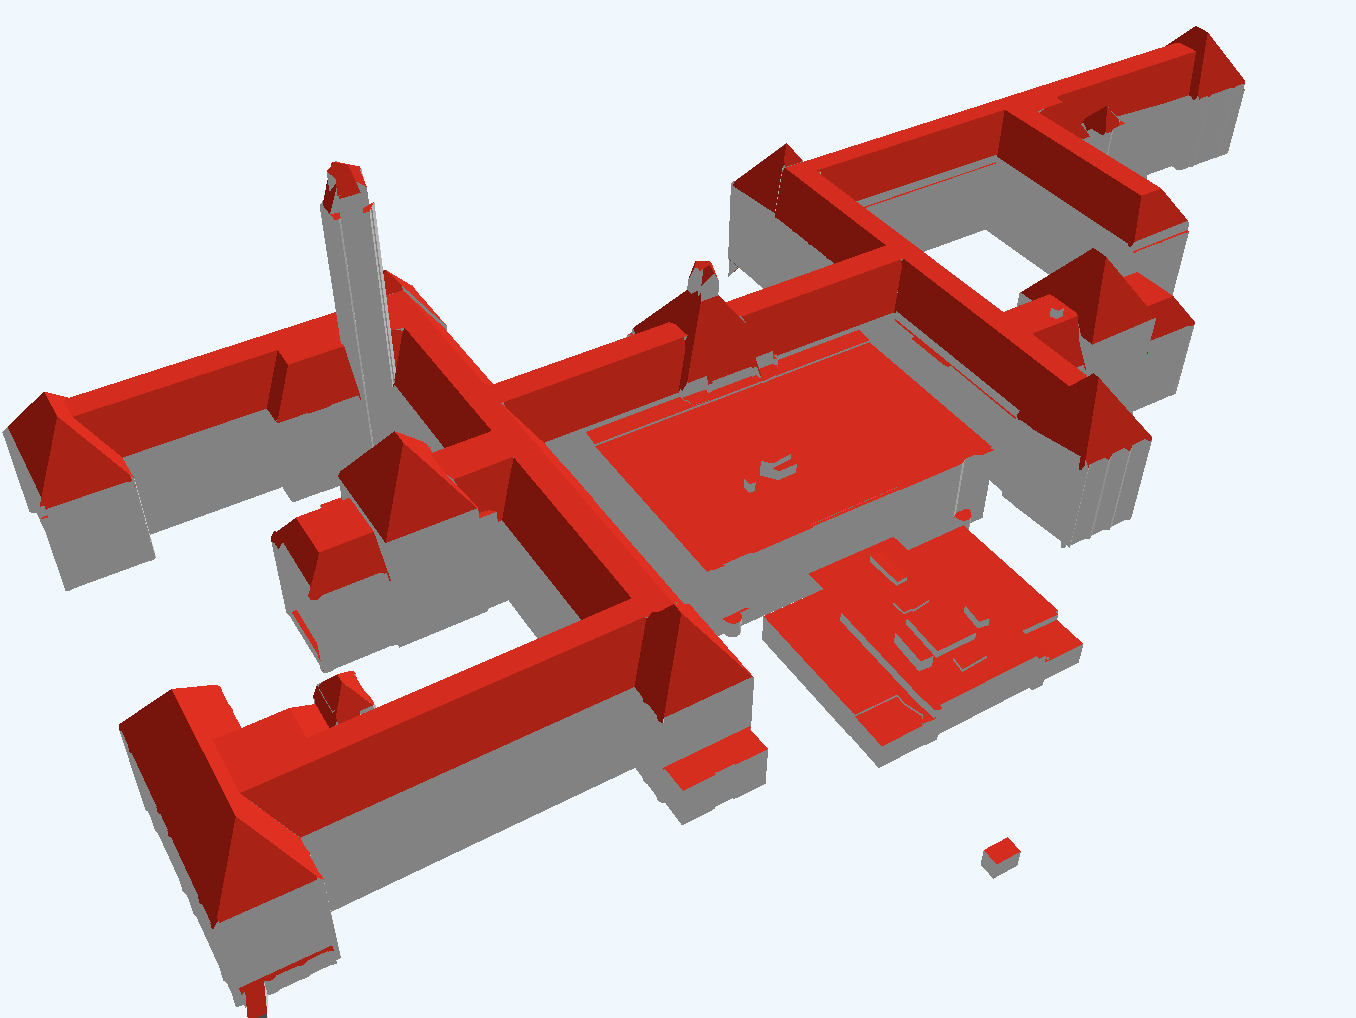
\includegraphics[width=\textwidth]{figs/result_analysis/tud_bk.png}
    \caption{TUD BK model (4549 vertices/feature)}
    \label{fig:tud_bk}
  \end{subfigure}
  \caption{Visual comparison of models with different geometric complexity.}
  \label{fig:geometry_comparison}
\end{figure}

The results demonstrate that geometric complexity significantly affects compression efficiency, with FlatCityBuf achieving better compression for more intricate models. The TU Delft BK building model, containing 4549 vertices per feature, exhibits a higher compression rate of 26.06\% compared to the simpler model with 340 vertices at 14.94\%.

This differential appears to result from the expanding boundary field as geometry becomes more complex. FlatCityBuf employs a strongly typed representation of boundaries (using u32 integers) that maintains a constant size for encoding each vertex, whereas CityJSONSeq requires additional bytes due to its text-based format. This fundamental difference in geometry encoding becomes increasingly advantageous for FlatCityBuf as geometric complexity rises.

\subsubsection{Vertices and coordinates}
\label{result:overview:analysis_of_file_size_results:vertices_and_coordinates}

To investigate how coordinate scale affects file size, I conducted tests using identical cube geometries with different coordinate magnitudes. All test models represent the same simple cube shape with identical geometric complexity (8 vertices per feature), but the coordinate values are scaled to different magnitudes—ranging from single digits to millions—while maintaining the same spatial relationships. \autoref{tab:vertices_comparison} presents the results of this analysis, utilising the same base cube geometry as in \autoref{result:overview:analysis_of_file_size_results:attributes}.

\begin{table}[htbp]
  \centering
  \caption{Comparison of file sizes with varying coordinate scales.}
  \label{tab:vertices_comparison}
  \begin{tabular}{@{}lrrrr@{}}
    \toprule
    \textbf{Dataset} & \textbf{FlatCityBuf}$^{\text{(a)}}$ & \textbf{CityJSONSeq}$^{\text{(b)}}$ & \textbf{Compression} & \textbf{Scale} \\
    \midrule
    Cube (1) & \qty{476}{\byte} & \qty{370}{\byte} & $-28.65\%$ & 1 \\
    Cube (10) & \qty{476}{\byte} & \qty{459}{\byte} & $-3.70\%$ & 10 \\
    Cube (1k) & \qty{476}{\byte} & \qty{507}{\byte} & $6.11\%$ & 1,000 \\
    Cube (1M) & \qty{476}{\byte} & \qty{579}{\byte} & $17.79\%$ & 1,000,000 \\
    \bottomrule
  \end{tabular}
  \begin{tablenotes}[flushleft]
    \footnotesize
  \item[a] Average feature size in bytes in FlatCityBuf: $\frac{\text{Total FlatCityBuf size}}{\text{Number of features}}$
  \item[b] Average feature size in bytes in CityJSONSeq: $\frac{\text{Total CityJSONSeq size}}{\text{Number of features}}$
  \end{tablenotes}
\end{table}

The results reveal an intriguing relationship between coordinate scale and file size in both formats. FlatCityBuf maintains a consistent size of 476 bytes regardless of coordinate magnitude, demonstrating its fixed-size binary encoding for numeric values. In contrast, CityJSONSeq's file size increases proportionally with larger coordinate values, growing from 370 bytes with single-digit coordinates to 579 bytes with million-scale coordinates.

This behaviour occurs because both FlatCityBuf and CityJSONSeq use integer values as coordinates, which are quantised by the \texttt{Transform} field as explained in \autoref{rw:cityjson:coordinate_quantisation}. However, FlatCityBuf stores these coordinates as fixed-size 32-bit integers, while CityJSONSeq, being a text-based format, requires more characters to represent larger numbers. Consequently, FlatCityBuf transitions from being less efficient than CityJSONSeq for small coordinate values (-28.65\%) to substantially more efficient for large coordinate values (17.79\%).

This characteristic explains the pattern observed in \autoref{result:overview:filesize_comparison}. FlatCityBuf demonstrates lower storage efficiency for PLATEAU datasets, likely because these datasets employ geographic coordinate systems with values typically between -180 and 180. Since CityJSON quantises coordinates through the \texttt{Transform} field, latitude and longitude values can be represented as relatively small integers. Conversely, datasets where FlatCityBuf performs better—such as NYC and Helsinki—use local coordinate systems (in metres) with larger internal values, resulting in improved compression efficiency with FlatCityBuf.

\subsubsection{Summary of File Size Analysis}
\label{result:overview:analysis_of_file_size_results:summary}

The comprehensive analysis of various factors affecting file size reveals distinct patterns in the compression performance of FlatCityBuf compared to CityJSONSeq:

\begin{itemize}
  \item \textbf{Level of Detail:} The analysis demonstrates that geometric detail levels have minimal impact on compression efficiency. While file sizes naturally increase with higher \ac{lod}s, the compression advantage of FlatCityBuf remains relatively consistent at approximately 24-25\% across different levels of geometric complexity.

  \item \textbf{Attribute Quantity:} The number of attributes significantly influences compression performance. FlatCityBuf's efficiency increases dramatically with attribute count, from minimal compression (5.07\%) with 10 attributes to substantial compression (44.13\%) with 1000 attributes. This progressive advantage stems from FlatCityBuf's schema-based approach that eliminates redundant attribute key storage.

  \item \textbf{Geometric Complexity:} More intricate geometries benefit from improved compression with FlatCityBuf. As boundary fields expand with geometric complexity, FlatCityBuf's fixed-size numeric representation provides greater efficiency compared to the text-based encoding of CityJSONSeq, increasing compression from 14.94\% for simple geometries to 26.06\% for complex models.

  \item \textbf{Coordinate Scale:} The magnitude of coordinate values has a significant impact on compression efficiency. FlatCityBuf's constant-size integer representation maintains consistent file sizes regardless of coordinate scale, while CityJSONSeq requires more space for larger values. This creates a transition from inferior compression (-28.65\%) with small coordinate values to superior compression (17.79\%) with large coordinate values.
\end{itemize}

These findings elucidate the observed variations in compression performance across different datasets in \autoref{tab:dataset_comparison}. FlatCityBuf demonstrates optimal performance for datasets with numerous attributes, complex geometries, and large-scale coordinate systems, while CityJSONSeq may retain advantages for simpler datasets with limited attributes and smaller coordinate values.

\section{Benchmark on Local Environment}
\label{result:benchmark_on_local_environment}

This section presents a comprehensive performance evaluation of the FlatCityBuf format conducted in a controlled local environment. The analysis focuses on critical metrics including read operations, memory utilisation, and processing efficiency to establish a thorough understanding of the format's performance characteristics.

\subsection{Test Environment}
\label{result:benchmark_on_local_environment:test_environment}

All benchmarks were executed within a consistent hardware and software configuration to ensure reliability and reproducibility:

\begin{itemize}
  \item \textbf{Hardware:} Apple MacBook Pro with M1 Max chip, 32GB unified memory
  \item \textbf{Operating System:} macOS Sequoia 15.4
  \item \textbf{Storage:} 1TB SSD with approximately 200GB available capacity
  \item \textbf{Runtime Environment:} Rust 1.86.0, with optimised release builds
\end{itemize}

\subsection{Measurement Parameters}
\label{result:benchmark_on_local_environment:measurement_parameters}

The benchmark framework captured multiple performance dimensions through the following key indicators:
\todo{Ravi's comment "you could also look at write performance here"}

\begin{itemize}
  \item \textbf{Read Performance:} Time required to deserialise the file and map the data into memory using zero-copy techniques, measured in milliseconds with microsecond precision

  \item \textbf{Memory Efficiency:} Peak Resident Set Size (RSS) during file processing, providing an accurate measurement of maximum memory requirements

\end{itemize}
These parameters were systematically measured across all encoding formats—CityJSONSeq, CBOR, BSON, and FlatCityBuf—to facilitate direct performance comparisons. CBOR and BSON were selected as additional comparison formats because they are JSON-compatible binary encoding formats, providing a meaningful intermediate comparison between text-based CityJSONSeq and the custom FlatCityBuf implementation. For CBOR and BSON evaluation, single CityJSON files were encoded, which serve as the source for the corresponding CityJSONSeq datasets. Other data formats such as Protocol Buffers or GeoParquet would require developing dedicated libraries similar to the FlatBuffers implementation, making them less suitable for this comparative analysis. The subsequent sections present a detailed analysis of these measurements and their implications for practical applications.

\subsection{Read Performance FlatCityBuf vs CityJSONSeq}
\label{result:benchmark_on_local_environment:read_performance_flatcitybuf_vs_cityjsonseq}

The performance comparison between FlatCityBuf and CityJSONSeq was conducted across multiple datasets, measuring processing time, and memory consumption as key metrics. \autoref{tab:performance_comparison} presents these results.

\begin{table}[ht]
  \centering
  \begin{threeparttable}
    \caption{Performance comparison between CityJSONSeq and FlatCityBuf}
    \label{tab:performance_comparison}
    \setlength{\tabcolsep}{10pt}
    \scriptsize
    \begin{tabular}{@{}l|rrr|rrr@{}}
      \toprule
      & \multicolumn{3}{c|}{\textbf{Processing Time}}
      & \multicolumn{3}{c}{\textbf{Memory Consumption}} \\
      \cmidrule(lr){2-4} \cmidrule(lr){5-7}
      \textbf{Dataset}
      & \textbf{cjseq\tnote{a}} & \textbf{FlatCityBuf} & \textbf{Ratio\tnote{b}}
      & \textbf{cjseq\tnote{a}} & \textbf{FlatCityBuf} & \textbf{Ratio\tnote{b}} \\
      \midrule
      3DBAG
      & \qty{56.3}{\milli\second} & \qty{6.6}{\milli\second} & 8.6$\times$
      & \qty{23.9}{\mega\byte} & \qty{5.1}{\mega\byte} & 4.7$\times$ \\

      3DBV
      & \qty{3.99}{\second} & \qty{122.5}{\milli\second} & 32.6$\times$
      & \qty{283.8}{\mega\byte} & \qty{63.2}{\mega\byte} & 4.5$\times$ \\

      Helsinki
      & \qty{4.05}{\second} & \qty{132.2}{\milli\second} & 30.6$\times$
      & \qty{15.3}{\mega\byte} & \qty{5.2}{\mega\byte} & 2.9$\times$ \\

      Ingolstadt
      & \qty{37.2}{\milli\second} & \qty{0.5}{\milli\second} & 75.8$\times$
      & \qty{30.1}{\mega\byte} & \qty{6.9}{\mega\byte} & 4.4$\times$ \\

      Montréal
      & \qty{50.3}{\milli\second} & \qty{0.6}{\milli\second} & 81.6$\times$
      & \qty{36.3}{\mega\byte} & \qty{5.7}{\mega\byte} & 6.4$\times$ \\

      NYC
      & \qty{887.6}{\milli\second} & \qty{42.9}{\milli\second} & 20.7$\times$
      & \qty{20.6}{\mega\byte} & \qty{5.0}{\mega\byte} & 4.1$\times$ \\

      Rotterdam
      & \qty{22.2}{\milli\second} & \qty{1.3}{\milli\second} & 17.6$\times$
      & \qty{9.2}{\mega\byte} & \qty{4.4}{\mega\byte} & 2.1$\times$ \\

      Vienna
      & \qty{45.9}{\milli\second} & \qty{1.9}{\milli\second} & 24.0$\times$
      & \qty{14.6}{\mega\byte} & \qty{5.2}{\mega\byte} & 2.8$\times$ \\

      Zürich
      & \qty{1.88}{\second} & \qty{151.9}{\milli\second} & 12.4$\times$
      & \qty{31.3}{\mega\byte} & \qty{5.1}{\mega\byte} & 6.2$\times$ \\

      PLATEAU (Building)
      & \qty{861.4}{\milli\second} & \qty{32.5}{\milli\second} & 26.5$\times$
      & \qty{220.9}{\mega\byte} & \qty{64.4}{\mega\byte} & 3.4$\times$ \\

      PLATEAU (Bridge)
      & \qty{83.9}{\milli\second} & \qty{0.3}{\milli\second} & 256.8$\times$
      & \qty{75.0}{\mega\byte} & \qty{12.0}{\mega\byte} & 6.3$\times$ \\

      PLATEAU (Railway)
      & \qty{37.9}{\milli\second} & \qty{2.0}{\milli\second} & 18.5$\times$
      & \qty{19.0}{\mega\byte} & \qty{5.1}{\mega\byte} & 3.8$\times$ \\

      PLATEAU (Transport)
      & \qty{244.0}{\milli\second} & \qty{13.3}{\milli\second} & 18.4$\times$
      & \qty{76.7}{\mega\byte} & \qty{20.2}{\mega\byte} & 3.8$\times$ \\

      PLATEAU (Tunnels)
      & \qty{47.9}{\milli\second} & \qty{1.9}{\milli\second} & 24.9$\times$
      & \qty{70.6}{\mega\byte} & \qty{12.6}{\mega\byte} & 5.6$\times$ \\

      PLATEAU (Vegetation)
      & \qty{852.3}{\milli\second} & \qty{32.9}{\milli\second} & 25.9$\times$
      & \qty{189.8}{\mega\byte} & \qty{56.9}{\mega\byte} & 3.3$\times$ \\

      \bottomrule
    \end{tabular}
    \begin{tablenotes}[flushleft]
      \footnotesize
    \item[a] CityJSONSeq
    \item[b] Ratio = CityJSONSeq metric / FlatCityBuf metric (higher values indicate better FlatCityBuf performance)
    \end{tablenotes}
  \end{threeparttable}
\end{table}

The performance comparison reveals significant advantages for FlatCityBuf in both processing time and memory consumption. FlatCityBuf demonstrates consistently superior performance, processing data between 8.6$\times$ and 256.8$\times$ faster than CityJSONSeq across all datasets. The most dramatic improvements are observed for the PLATEAU bridge model and Ingolstadt datasets, which suggests that FlatCityBuf exhibits lower overhead when handling smaller datasets. Memory consumption is also consistently reduced compared to CityJSONSeq, with FlatCityBuf showing particularly notable advantages for certain datasets, including Montréal and the PLATEAU Bridge model.

\subsection{Read performance FlatCityBuf vs CBOR}
\label{result:benchmark_on_local_environment:read_performance_flatcitybuf_vs_cbor}

The performance comparison between FlatCityBuf and CBOR was conducted using the same datasets and measurement methodology. \autoref{tab:performance_comparison_cbor} presents these results.

\begin{table}[ht]
  \centering
  \begin{threeparttable}
    \caption{Performance comparison between CBOR and FlatCityBuf}
    \label{tab:performance_comparison_cbor}
    \setlength{\tabcolsep}{10pt}
    \scriptsize
    \begin{tabular}{@{}l|rrr|rrr@{}}
      \toprule
      & \multicolumn{3}{c|}{\textbf{Processing Time}}
      & \multicolumn{3}{c}{\textbf{Memory Consumption}} \\
      \cmidrule(lr){2-4} \cmidrule(lr){5-7}
      \textbf{Dataset}
      & \textbf{CBOR} & \textbf{FlatCityBuf} & \textbf{Ratio\tnote{a}}
      & \textbf{CBOR} & \textbf{FlatCityBuf} & \textbf{Ratio\tnote{a}} \\
      \midrule
      3DBAG
      & \qty{74.0}{\milli\second} & \qty{6.6}{\milli\second} & 11.2$\times$
      & \qty{194.1}{\mega\byte} & \qty{5.1}{\mega\byte} & 38.1$\times$ \\

      3DBV
      & \qty{6.34}{\second} & \qty{122.5}{\milli\second} & 51.8$\times$
      & \qty{4.96}{\giga\byte} & \qty{63.2}{\mega\byte} & 80.3$\times$ \\

      Helsinki
      & \qty{7.97}{\second} & \qty{132.2}{\milli\second} & 60.3$\times$
      & \qty{5.14}{\giga\byte} & \qty{5.2}{\mega\byte} & 1011.2$\times$ \\

      Ingolstadt
      & \qty{46.9}{\milli\second} & \qty{0.5}{\milli\second} & 95.7$\times$
      & \qty{187.5}{\mega\byte} & \qty{6.9}{\mega\byte} & 27.3$\times$ \\

      Montréal
      & \qty{58.4}{\milli\second} & \qty{0.6}{\milli\second} & 94.7$\times$
      & \qty{257.1}{\mega\byte} & \qty{5.7}{\mega\byte} & 45.3$\times$ \\

      NYC
      & \qty{1.33}{\second} & \qty{42.9}{\milli\second} & 31.0$\times$
      & \qty{1.65}{\giga\byte} & \qty{5.0}{\mega\byte} & 337.4$\times$ \\

      Rotterdam
      & \qty{30.8}{\milli\second} & \qty{1.3}{\milli\second} & 24.4$\times$
      & \qty{140.0}{\mega\byte} & \qty{4.4}{\mega\byte} & 31.9$\times$ \\

      Vienna
      & \qty{58.8}{\milli\second} & \qty{1.9}{\milli\second} & 30.7$\times$
      & \qty{179.8}{\mega\byte} & \qty{5.2}{\mega\byte} & 34.7$\times$ \\

      Zürich
      & \qty{3.53}{\second} & \qty{151.9}{\milli\second} & 23.3$\times$
      & \qty{4.51}{\giga\byte} & \qty{5.1}{\mega\byte} & 913.2$\times$ \\

      PLATEAU (Building)
      & \qty{1.06}{\second} & \qty{32.5}{\milli\second} & 32.4$\times$
      & \qty{1.83}{\giga\byte} & \qty{64.4}{\mega\byte} & 28.4$\times$ \\

      PLATEAU (Bridge)
      & \qty{63.6}{\milli\second} & \qty{0.3}{\milli\second} & 194.7$\times$
      & \qty{305.4}{\mega\byte} & \qty{12.0}{\mega\byte} & 25.6$\times$ \\

      PLATEAU (Railway)
      & \qty{46.3}{\milli\second} & \qty{2.0}{\milli\second} & 22.7$\times$
      & \qty{141.0}{\mega\byte} & \qty{5.1}{\mega\byte} & 27.9$\times$ \\

      PLATEAU (Transport)
      & \qty{316.1}{\milli\second} & \qty{13.3}{\milli\second} & 23.8$\times$
      & \qty{614.5}{\mega\byte} & \qty{20.2}{\mega\byte} & 30.5$\times$ \\

      PLATEAU (Tunnels)
      & \qty{147.7}{\milli\second} & \qty{1.9}{\milli\second} & 76.7$\times$
      & \qty{400.2}{\mega\byte} & \qty{12.6}{\mega\byte} & 31.8$\times$ \\

      PLATEAU (Vegetation)
      & \qty{997.8}{\milli\second} & \qty{32.9}{\milli\second} & 30.3$\times$
      & \qty{1.97}{\giga\byte} & \qty{56.9}{\mega\byte} & 35.3$\times$ \\

      \bottomrule
    \end{tabular}
    \begin{tablenotes}[flushleft]
      \footnotesize
    \item[a] Ratio = CBOR metric / FlatCityBuf metric (higher values indicate better FlatCityBuf performance)
    \end{tablenotes}
  \end{threeparttable}
\end{table}

The benchmark results demonstrate that FlatCityBuf consistently outperforms CBOR across all tested datasets. When compared to CBOR, FlatCityBuf achieved processing time improvements ranging from 11.2$\times$ to 194.7$\times$, with particularly significant speedups observed for smaller datasets such as the PLATEAU bridge model and Ingolstadt. This pattern reflects FlatCityBuf's zero-copy deserialization advantage, which provides proportionally greater benefits when parsing overhead dominates the total processing time in smaller datasets.

Memory consumption was reduced by factors ranging from 25.6$\times$ to 1011.2$\times$, with the most dramatic improvements observed in larger datasets such as Helsinki and Zürich. This trend occurs because CBOR requires loading the entire dataset into memory during deserialization, while FlatCityBuf's zero-copy approach allows selective access without full memory allocation. As dataset size increases, this fundamental difference in memory management strategy becomes increasingly pronounced.

\subsection{Read performance FlatCityBuf vs BSON}
\label{result:benchmark_on_local_environment:read_performance_flatcitybuf_vs_bson}

The performance comparison between FlatCityBuf and BSON followed the same methodology as the previous comparisons. \autoref{tab:performance_comparison_bson} presents the detailed results.

\begin{table}[ht]
  \centering
  \begin{threeparttable}
    \caption{Performance comparison between BSON and FlatCityBuf}
    \label{tab:performance_comparison_bson}
    \setlength{\tabcolsep}{10pt}
    \scriptsize
    \begin{tabular}{@{}l|rrr|rrr@{}}
      \toprule
      & \multicolumn{3}{c|}{\textbf{Processing Time}}
      & \multicolumn{3}{c}{\textbf{Memory Consumption}} \\
      \cmidrule(lr){2-4} \cmidrule(lr){5-7}
      \textbf{Dataset}
      & \textbf{BSON} & \textbf{FlatCityBuf} & \textbf{Ratio\tnote{a}}
      & \textbf{BSON} & \textbf{FlatCityBuf} & \textbf{Ratio\tnote{a}} \\
      \midrule
      3DBAG
      & \qty{117.1}{\milli\second} & \qty{6.6}{\milli\second} & 17.8$\times$
      & \qty{276.8}{\mega\byte} & \qty{5.1}{\mega\byte} & 54.3$\times$ \\

      3DBV
      & \qty{9.97}{\second} & \qty{122.5}{\milli\second} & 81.4$\times$
      & \qty{6.38}{\giga\byte} & \qty{63.2}{\mega\byte} & 103.4$\times$ \\

      Helsinki
      & \qty{14.64}{\second} & \qty{132.2}{\milli\second} & 110.7$\times$
      & \qty{6.77}{\giga\byte} & \qty{5.2}{\mega\byte} & 1331.7$\times$ \\

      Ingolstadt
      & \qty{79.9}{\milli\second} & \qty{0.5}{\milli\second} & 163.1$\times$
      & \qty{267.3}{\mega\byte} & \qty{6.9}{\mega\byte} & 38.9$\times$ \\

      Montréal
      & \qty{151.3}{\milli\second} & \qty{0.6}{\milli\second} & 245.5$\times$
      & \qty{445.5}{\mega\byte} & \qty{5.7}{\mega\byte} & 78.6$\times$ \\

      NYC
      & \qty{1.78}{\second} & \qty{42.9}{\milli\second} & 41.5$\times$
      & \qty{2.50}{\giga\byte} & \qty{5.0}{\mega\byte} & 510.7$\times$ \\

      Rotterdam
      & \qty{67.6}{\milli\second} & \qty{1.3}{\milli\second} & 53.5$\times$
      & \qty{265.1}{\mega\byte} & \qty{4.4}{\mega\byte} & 60.4$\times$ \\

      Vienna
      & \qty{82.0}{\milli\second} & \qty{1.9}{\milli\second} & 42.9$\times$
      & \qty{239.8}{\mega\byte} & \qty{5.2}{\mega\byte} & 46.2$\times$ \\

      Zürich
      & \qty{5.80}{\second} & \qty{151.9}{\milli\second} & 38.2$\times$
      & \qty{6.97}{\giga\byte} & \qty{5.1}{\mega\byte} & 1409.0$\times$ \\

      PLATEAU (Building)
      & \qty{2.37}{\second} & \qty{32.5}{\milli\second} & 72.7$\times$
      & \qty{3.76}{\giga\byte} & \qty{64.4}{\mega\byte} & 58.4$\times$ \\

      PLATEAU (Bridge)
      & \qty{177.0}{\milli\second} & \qty{0.3}{\milli\second} & 541.8$\times$
      & \qty{500.2}{\mega\byte} & \qty{12.0}{\mega\byte} & 41.9$\times$ \\

      PLATEAU (Railway)
      & \qty{80.5}{\milli\second} & \qty{2.0}{\milli\second} & 39.4$\times$
      & \qty{294.0}{\mega\byte} & \qty{5.1}{\mega\byte} & 58.1$\times$ \\

      PLATEAU (Transport)
      & \qty{603}{\milli\second} & \qty{14}{\milli\second} & 43.1$\times$
      & \qty{1.0}{\giga\byte} & \qty{23.0}{\mega\byte} & 46.0$\times$ \\

      PLATEAU (Tunnels)
      & \qty{251}{\milli\second} & \qty{2}{\milli\second} & 125.5$\times$
      & \qty{618.4}{\mega\byte} & \qty{14.2}{\mega\byte} & 43.5$\times$ \\

      PLATEAU (Vegetation)
      & \qty{2.07}{\second} & \qty{33}{\milli\second} & 65.3$\times$
      & \qty{3.99}{\giga\byte} & \qty{70.4}{\mega\byte} & 71.8$\times$ \\

      \bottomrule
    \end{tabular}
    \begin{tablenotes}[flushleft]
      \footnotesize
    \item[a] Ratio = BSON metric / FlatCityBuf metric (higher values indicate better FlatCityBuf performance)
    \end{tablenotes}
  \end{threeparttable}
\end{table}

The benchmark results show that FlatCityBuf significantly outperforms BSON across all tested datasets. Processing time improvements ranged from 17.8$\times$ to 541.8$\times$, with the most dramatic speedup observed for the PLATEAU bridge model. The exceptional performance gain for smaller datasets like PLATEAU bridge model reflects FlatCityBuf's zero-copy deserialization advantage, where parsing overhead represents a larger proportion of total processing time.

Memory consumption was reduced by factors ranging from 38.9$\times$ to 1409.0$\times$, with the largest improvements seen in datasets such as Zürich and Helsinki. This substantial memory efficiency stems from BSON's requirement to deserialize the entire document into memory structures, while FlatCityBuf enables direct access to data without full memory allocation. The performance gains are generally more pronounced than those observed in the CBOR comparison.

\subsection{Summary of local environment benchmark}
\label{result:benchmark_on_local_environment:summary}
To summarise the results of the local environment benchmark, FlatCityBuf demonstrates significant performance improvements across all tested formats and datasets, with varying degrees of enhancement depending on the comparison format and dataset characteristics.

\begin{itemize}
  \item Processing time: Processing time improvements represent the primary objective of this research. Compared to CityJSONSeq, FlatCityBuf achieved speedups ranging from 8.6$\times$ (3DBAG) to 256.8$\times$ (PLATEAU bridge model). Against CBOR, improvements ranged from 11.2$\times$ (3DBAG) to 194.7$\times$ (PLATEAU bridge model). For BSON, the most dramatic gains were observed, ranging from 17.8$\times$ (3DBAG) to 541.8$\times$ (PLATEAU bridge model). Generally, smaller datasets exhibit higher performance ratios, while larger datasets show significant absolute time savings despite lower ratios.

  \item Memory consumption: Memory efficiency improvements varied significantly across formats. Compared to CityJSONSeq, FlatCityBuf achieved reductions ranging from 1.9$\times$ (Rotterdam) to 6.3$\times$ (PLATEAU bridge model). Against CBOR, memory consumption was reduced by factors of 27.3$\times$ to 1011.2$\times$, with the largest improvements in datasets like Helsinki and Zürich. For BSON, memory reductions ranged from 38.9$\times$ to 1409.0$\times$, with exceptional efficiency gains in large datasets. It should be noted that memory consumption comparisons with CBOR and BSON formats are not entirely equitable, as these formats require encoding and loading entire datasets into memory, while both FlatCityBuf and CityJSONSeq support streaming operations that enable incremental data processing without full memory allocation.
\end{itemize}

\section{Benchmark over the web}
\label{result:benchmark_over_the_web}
To evaluate FlatCityBuf's performance in real-world web scenarios, we compared it with the 3DBAG \ac{api} \citep{3dbag_api}. The 3DBAG \ac{api} currently supports two query types: \textit{feature ID query} for retrieving CityJSONFeature by identifier (\eg, \texttt{identificatie} attribute of 3DBAG) and \textit{bounding box query} for spatial queries with configurable result limits via the \texttt{limit} parameter.

While network-based benchmarking provides more realistic performance insights, it introduces additional complexity due to variable network latency and server-side factors. As discussed in \autoref{result:cross_platform_implementation:cloud_integration}, FlatCityBuf operates without server-side processing, requiring only static file storage, contrasting with traditional application and database servers.

We acknowledge that this comparison is not entirely equitable due to fundamental architectural differences and the 3DBAG \ac{api} being a public service potentially handling concurrent requests. However, this comparison remains valuable as API-based access represents the current standard approach for CityJSON data consumption in web applications.

\subsection{Benchmark environment}
\label{result:benchmark_over_the_web:benchmark_environment}

For the web-based benchmark, we used the 3DBAG dataset. The FlatCityBuf implementation utilised a static file encoding the entire Netherlands dataset, resulting in a 70.4 GB file containing all features, attribute indices for all attributes, and spatial indexing. Data retrieval was performed using a Rust program with HTTP range requests (browser-based testing was avoided due to disk caching effects). The 3DBAG \ac{api}, publicly available at \url{https://api.3dbag.nl/}, operates on a Flask backend with PostgreSQL and PostGIS extension for database management \citep{powalka_2023}.

To account for network variability and potential outliers, we collected 100 samples for each method with 10 warmup samples.

\subsection{Feature ID query}
\label{result:benchmark_over_the_web:feature_id_query}

Both FlatCityBuf files and the 3DBAG \ac{api} database organise features according to technical implementation decisions (\eg, FlatCityBuf features are typically sorted by Hilbert curve). To ensure fair comparison by identifier, we selected 5 features distributed across different regions of the Netherlands, representing landmark or well-known buildings. The benchmark results represent the average performance across 100 samples for all 5 features.

\autoref{tab:feature_id_performance} presents the performance comparison between FlatCityBuf and the 3DBAG \ac{api} for feature ID queries. Overall, FlatCityBuf demonstrates approximately 2.1$\times$ faster performance than the 3DBAG \ac{api} for identifier-based feature retrieval. Performance ranged from 2.7$\times$ faster (Groningen station) to 1.5$\times$ faster (Eindhoven station).

\begin{table}[ht]
  \centering
  \caption{Feature ID query performance comparison between FlatCityBuf and 3DBAG API}
  \label{tab:feature_id_performance}
  \resizebox{\textwidth}{!}{%
    \begin{tabular}{llccc}
      \toprule
      \textbf{Feature ID} & \textbf{Location} & \textbf{FCB\tnote{a}} & \textbf{API\tnote{b}} & \textbf{Ratio\tnote{c}} \\
      & & \textbf{(ms)} & \textbf{(ms)} & \\
      \midrule
      NL.IMBAG.Pand.0503100000032914 & TU Delft BK building & 935.8 & 2412.5 & 2.6$\times$ \\
      NL.IMBAG.Pand.0363100012185598 & Amsterdam Central Station & 858.0 & 2106.7 & 2.5$\times$ \\
      NL.IMBAG.Pand.0014100010938997 & Groningen Station & 821.7 & 2254.8 & 2.7$\times$ \\
      NL.IMBAG.Pand.0772100000295227 & Eindhoven Station & 1378.7 & 2013.4 & 1.5$\times$ \\
      NL.IMBAG.Pand.0153100000261851 & Enschede Station & 1070.4 & 2058.8 & 1.9$\times$ \\
      \midrule
      \textbf{Average} & & \textbf{1012.9} & \textbf{2169.2} & \textbf{2.1$\times$} \\
      \bottomrule
    \end{tabular}%
  }

  \begin{tablenotes}[flushleft]
    \footnotesize
  \item[a] FCB = FlatCityBuf
  \item[b] API = 3DBAG \ac{api}
  \item[c] Ratio = 3DBAG \ac{api} / FlatCityBuf (higher values indicate better FlatCityBuf performance)
  \end{tablenotes}
\end{table}

\subsection{Bounding box query}
\label{result:benchmark_over_the_web:bounding_box_query}

For spatial query performance comparison, we selected a 2km $\times$ 2km bounding box around the Delft University of Technology campus, requesting the first 10 features within the area (matching the 3DBAG \ac{api}'s default limit). The benchmark results represent the average of 100 samples. The bounding box coordinates were \texttt{(84000.0, 444000.0, 86000.0, 446000.0)} in the Amersfoort / RD New + NAP height (EPSG:7415) coordinate system.

FlatCityBuf demonstrated approximately 15.1$\times$ faster performance than the 3DBAG \ac{api} for bounding box queries. This significant improvement over feature ID queries likely results from FlatCityBuf's Hilbert curve-based feature sorting, which enables spatially proximate features to be retrieved in batched operations.

\begin{table}[ht]
  \centering
  \caption{Bounding box query performance comparison between FlatCityBuf and 3DBAG API}
  \label{tab:bounding_box_performance}
  \begin{tabular}{lccc}
    \toprule
    \textbf{Query Type} & \textbf{FlatCityBuf} & \textbf{3DBAG API} & \textbf{Ratio\tnote{a}} \\
    & \textbf{(ms)} & \textbf{(ms)} & \\
    \midrule
    Bounding box (2km $\times$ 2km) & 492.6 & 7420.3 & 15.1$\times$ \\
    \bottomrule
  \end{tabular}
  \begin{tablenotes}[flushleft]
    \footnotesize
  \item[a] Ratio = 3DBAG API / FlatCityBuf (higher values indicate better FlatCityBuf performance)
  \end{tablenotes}
\end{table}

Despite the architectural differences between FlatCityBuf and the 3DBAG API, FlatCityBuf demonstrated superior performance across both query patterns. Notably, FlatCityBuf does not distinguish between identifier-based and attribute-based queries, as both utilize the same underlying mechanism. Consequently, we can expect similar performance characteristics for other attribute-based queries as well. These performance results highlight FlatCityBuf's potential for web application deployment.

\chapter{Discussion}
\label{chp:discussion}

This chapter discusses the implications of our experimental results and their broader significance for 3D city modelling applications.

\section{Use Cases of FlatCityBuf}
\label{use_case_flat_city_buffer}

This section examines the most appropriate application scenarios for the FlatCityBuf format based on its demonstrated performance characteristics.

\subsection{Flexible Data Download}
\label{flexible_data_download}

Providing users with the ability to download specific data of interest represents one of the most valuable applications of 3D city models, particularly within open data initiatives. Existing services such as 3DBAG offer download functionality for CityJSON data in various formats including CityJSON, OBJ, and GeoPackage. However, these services typically constrain users to downloading predefined tiles rather than precisely the data matching their specific requirements.

\citet{fcb-web-demo} demonstrates a web application that enables users to download precisely the data they require. This implementation successfully showcases FlatCityBuf's capability to facilitate targeted data retrieval. Through its attribute indexing mechanism, users can download filtered datasets based on specific criteria, such as features exceeding 100 metres in height.

\subsection{Data Analysis}
\label{data_analysis}
\todo{this is not too convincing to me yet. Why mention CFD specifically here? most resources in CFD will not be affected by using FCB, maybe only a bit in the data preprocessing? (converting from FCB to CFD specific geometry enciding)
Mayber a more interesting use case is the 3DBAG generation pipeline, where we have different stages that need to read/write cjseq files, and I/O is actually one of the bottlenecks (eg in conversion from fcb to 3d tiles)}
As demonstrated by the performance benchmarks, FlatCityBuf excels in read operations compared to alternative data formats, making it particularly suitable for analysing large-scale datasets. Computational Fluid Dynamics in urban environments, for instance, requires processing substantial volumes of detailed geometric data. Such analyses typically demand significant memory and computational resources. FlatCityBuf can process these data more efficiently by leveraging its zero-copy capability.

The format also simplifies analytical workflows. Conventional approaches to large-scale data processing often require chunking data across multiple files, necessitating additional programming to manage file aggregation. In contrast, FlatCityBuf encapsulates data in a single file that can be efficiently loaded and accessed, even in web-based environments, streamlining analytical processes.

\section{Impact on Server Architecture}
\label{affect_on_server_architecture}

FlatCityBuf introduces significant opportunities for simplifying server architectures for 3D city model delivery.

\subsection{Traditional Server Architecture}
\label{traditional_server_architecture}

Conventional server architectures for 3D city models typically employ both application and database servers. For example, \citet{3dcitydb} utilises PostgreSQL or Oracle as the database server with PostgREST API \citep{postgrest} providing data access through its toolchain. Similarly, the 3DBAG API uses PostgreSQL as its database server and Flask (Python) as the application server.

In contrast, FlatCityBuf operates as a static file, requiring only a basic HTTP server such as Nginx for data distribution. This approach aligns with modern cloud service offerings, where providers like AWS S3 and Google Cloud Storage offer optimised solutions for serving static content.

\subsection{Cloud Architecture Advantages}
\label{cloud_architecture_achieved}

\subsection{Scalability}
\label{scalability}

Scalability presents a significant challenge in traditional server architectures. These systems typically employ Relational Database Management Systems (RDBMS) that often encounter scaling limitations. Common mitigation strategies include sharding and replication (horizontal scaling) or resource expansion (vertical scaling), both requiring additional computational, memory, and storage resources.

FlatCityBuf circumvents these challenges by functioning as a static file that can leverage cloud providers' inherent scalability and high availability infrastructure. This characteristic offers substantial benefits for applications built on 3D city model data. Service providers can host static FlatCityBuf files on standard servers, allowing unrestricted access for various use cases without implementing the rate-limiting mechanisms often necessary with traditional server architectures.

\subsection{Cost-effectiveness}
\label{cost_effectiveness}

FlatCityBuf contributes significantly to operational cost-effectiveness. Although precise server costs vary according to specific use cases, hosting static files through cloud service providers is generally substantially more economical than maintaining dedicated database and application servers.

\todo{add more description of comparison}
\begin{figure}[htbp]
  \centering
  \begin{subfigure}[b]{0.48\textwidth}
    \centering
    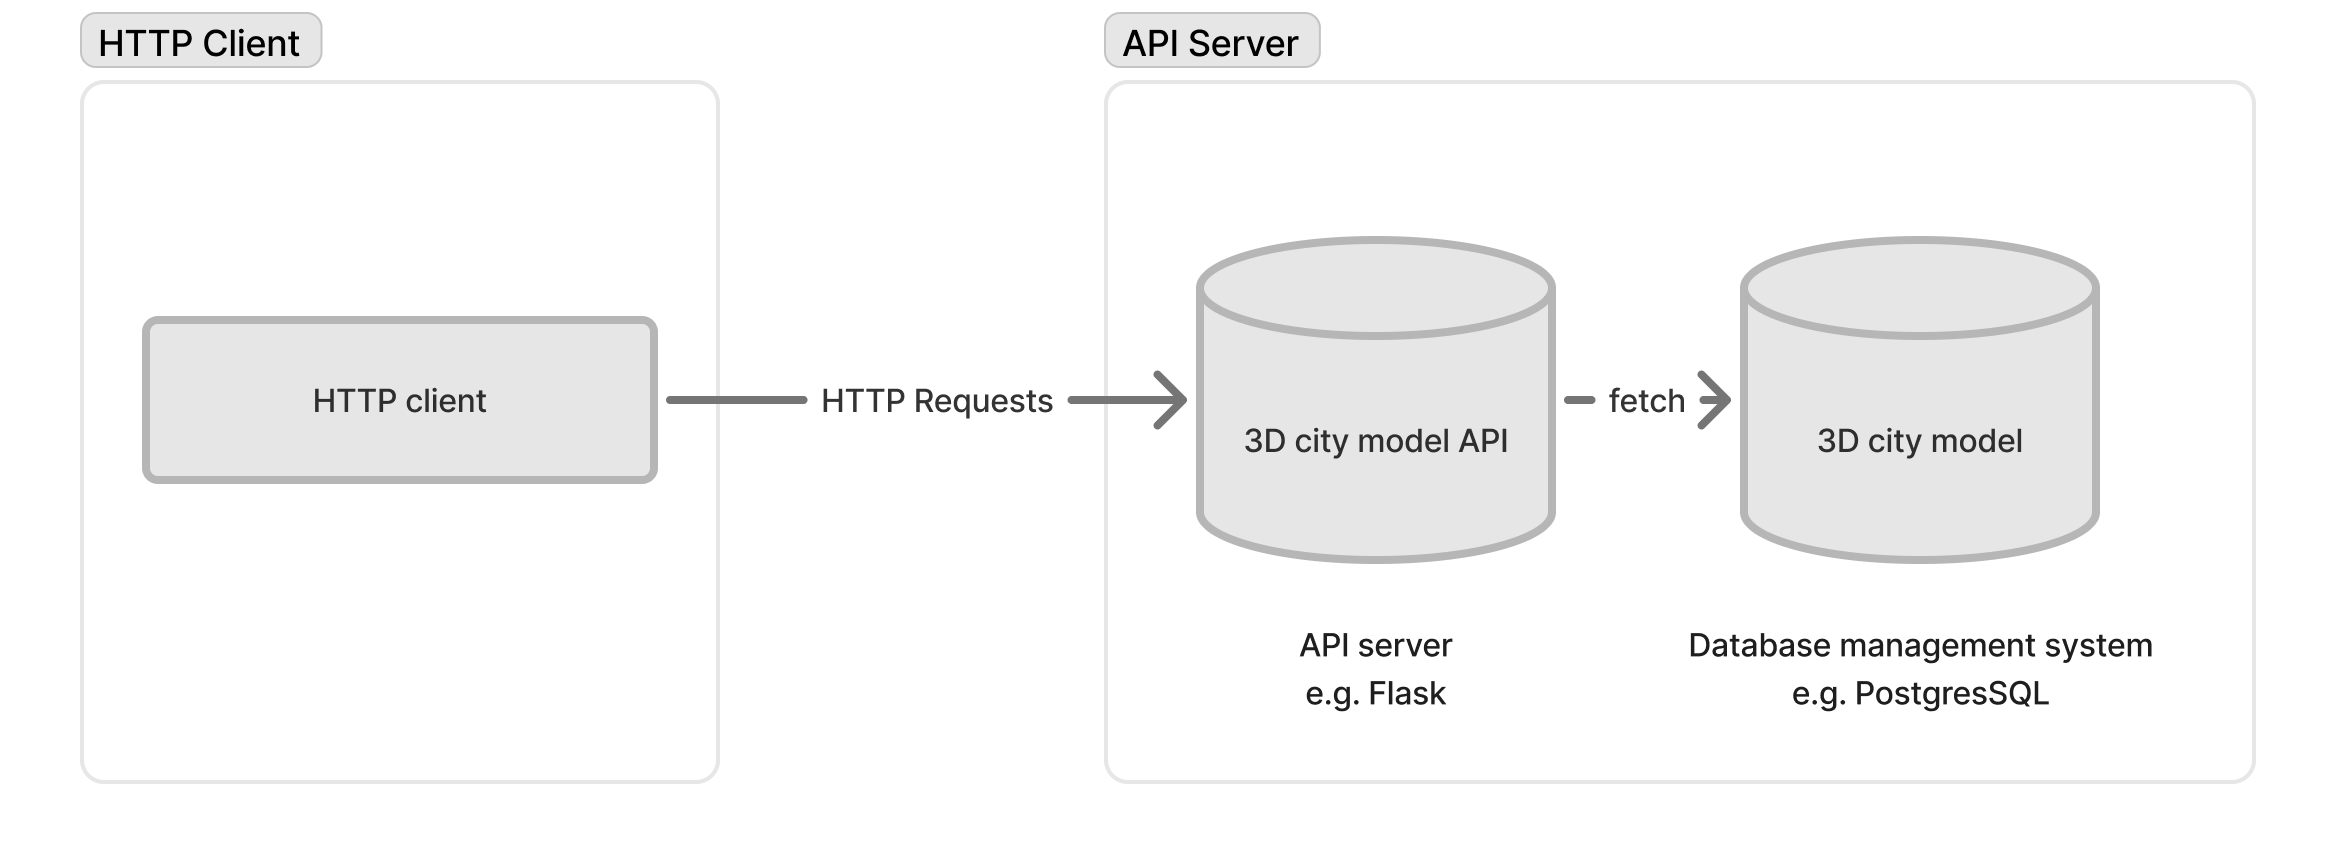
\includegraphics[width=\textwidth]{figs/discussion/server_architecture.png}
    \caption{Traditional server architecture with database and application servers}
    \label{fig:traditional_architecture}
  \end{subfigure}
  \hfill
  \begin{subfigure}[b]{0.48\textwidth}
    \centering
    \includegraphics[width=\textwidth]{figs/discussion/server_architecture_fcb.png}
    \caption{Simplified FlatCityBuf architecture}
    \label{fig:fcb_architecture}
  \end{subfigure}
  \caption{Comparison between traditional and FlatCityBuf server architectures. The proposed method eliminates the need for complex database infrastructure by leveraging static file hosting with built-in spatial and attribute indices.}
  \label{fig:architecture_comparison}
\end{figure}

\section{Limitations}
\label{limitations}

Despite its advantages in simplicity, scalability, and cost-effectiveness, FlatCityBuf does present certain limitations that warrant consideration.

\subsection{Query Flexibility}
\label{flexibility_of_query}

While FlatCityBuf supports both spatial and attribute indexing, its query capabilities remain more constrained than those of specialised spatial database applications. Traditional approaches employing RDBMS with spatial indexing provide more comprehensive query functionality. For instance, 3DCityDB enables filtering by LoD, CityObject type, and various other parameters, whereas FlatCityBuf primarily supports attribute-based filtering. Similarly, regarding spatial functions, 3DCityDB can utilise the extensive spatial capabilities of PostGIS, while FlatCityBuf currently only implements bounding box queries. Consequently, FlatCityBuf is optimised for scenarios requiring relatively straightforward filtering conditions.

\subsection{Client-side Application Complexity}
\label{complexity_of_client_side_application}

Although FlatCityBuf simplifies server architecture, it introduces additional complexity in client-side applications, which must implement logic for loading and processing the format. By comparison, OGC API and equivalent Web API services adhere to standardised designs that can be utilised by any client application—whether accessed through command-line interfaces, browsers, or mobile applications. While FlatCityBuf supports cross-platform applications, it requires language-specific or platform-specific library implementations.

\subsection{Update Complexity}
\label{ease_of_update}

Zero-copy data formats like FlatCityBuf generally present challenges for data updates due to their relatively rigid structure. Fixed-size data types such as integers or floating-point numbers cannot be dynamically converted to alternative types. Furthermore, since the format contains immutable spatial and attribute indices, updating the data necessitates rewriting the entire file. This characteristic renders FlatCityBuf less suitable for frequently updated datasets, positioning it instead as an optimal solution for data analysis and efficient download services.


\include{chapters/06_future_work}

\chapter{Conclusion}
\label{chp:conclusion}

\todo{write conclusion and future work}

\appendix

%%%
\cleardoublepage
%-- *mandatory* appendix about the reproducibility


\chapter{Reproducibility self-assessment}

\section{Marks for each of the criteria}

\begin{figure}[h]
  \centering
  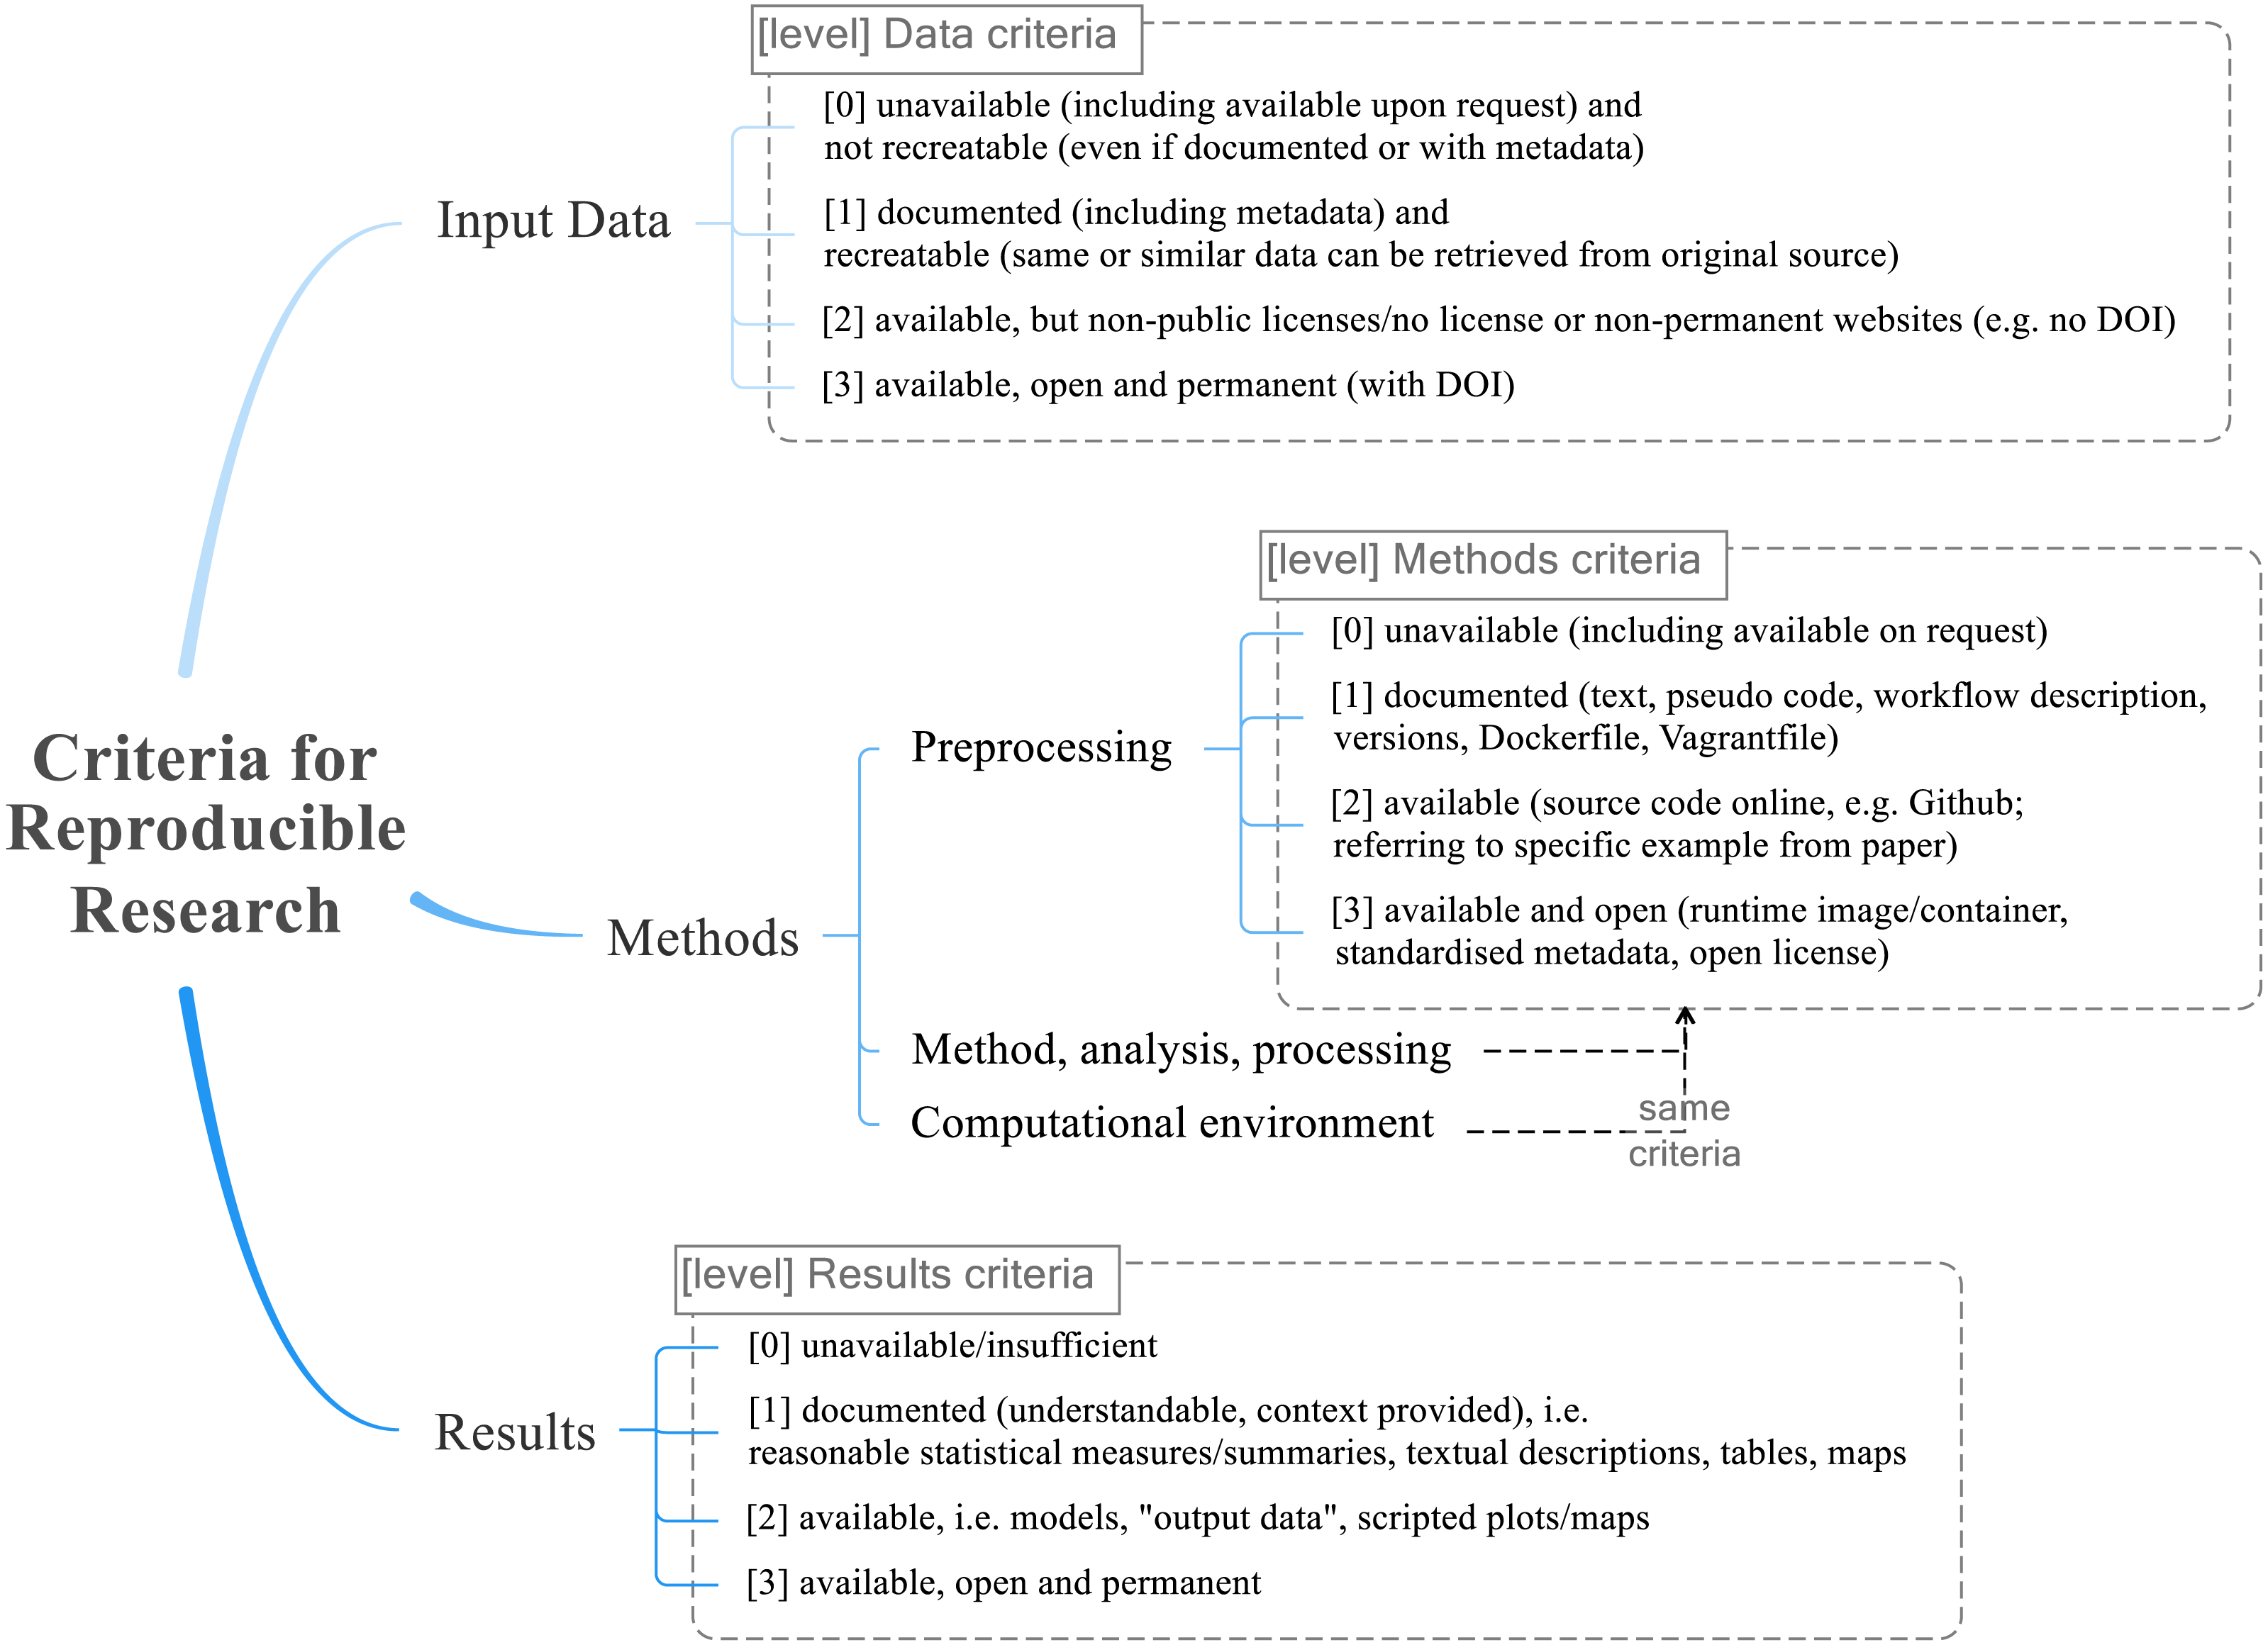
\includegraphics[width=0.8\linewidth]{figs/reproducibility_criteria.png}
  \caption{Reproducibility criteria to be assessed.}
\label{fig:reproducibility_criteria}
\end{figure}

Grade/evaluate yourself for the 5 criteria (giving 0/1/2/3 for each):
\begin{enumerate}
  \item input data
  \item preprocessing
  \item methods
  \item computational environment
  \item results
\end{enumerate}


%%%
\section{Self-reflection} 

A self-reflection about the reproducibility of your thesis/results.

We expect maximum 1 page here.

For example, if your data are not made publicly available, you need to justify it why (perhaps the company prevented you from doing this).

%-- other examples of Appendix, not mandatory


\chapter{Some UML diagrams}

\begin{figure}
  \centering
  % 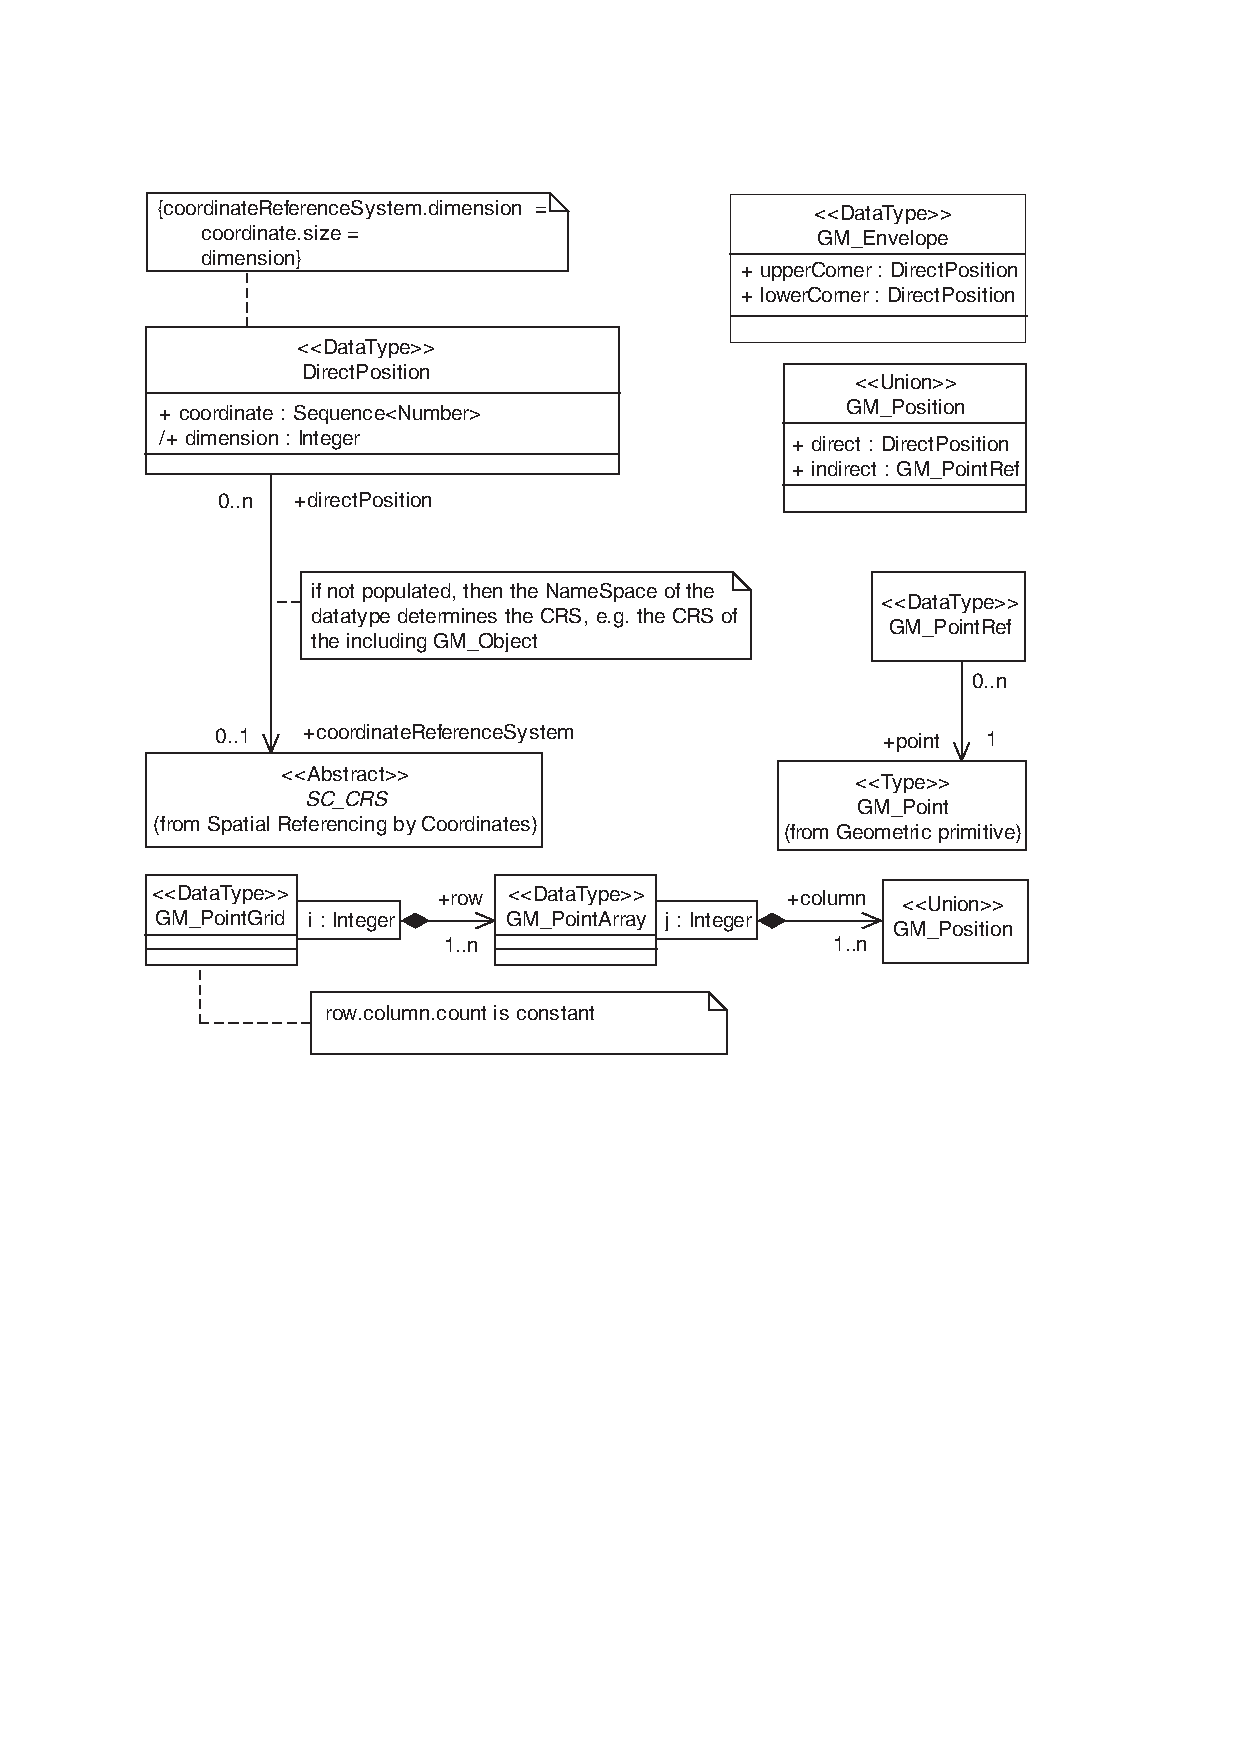
\includegraphics[width=0.8\linewidth]{figs/someuml.pdf}
  \caption{The UML diagram of something that looks important.}
\label{fig:someuml}
\end{figure}

\chapter{FlatCityBuf Schema}
\label{appendix:flatcitybuf_schema}

\section{Tables}

The package \texttt{booktabs} permits you to make nicer tables than the basic ones in \LaTeX.
See for instance \autoref{tab:example}.
\begin{table}
  \centering
  \begin{tabular}{@{}lrrcrrc@{}} \toprule
    & \multicolumn{2}{c}{3D model} && \multicolumn{2}{c}{input} \\
    \cmidrule{2-3}  \cmidrule{5-6}
    & solids & faces && vertices & constraints  \\
    \toprule
    \textbf{campus}  & 370   & 4~298  && 5~970  & 3~976   \\
    \textbf{kvz}     & 637   & 6~549  && 8~951  & 13~571  \\
    \textbf{engelen} & 1~629 & 15~870 && 23~732 & 15~868 \\
    \bottomrule
   \end{tabular}
  \caption{Details concerning the datasets used for the experiments.}%
\label{tab:example}
\end{table}


% *****************************************************************
% Backmatter
%******************************************************************
\backmatter

%- bibliography
\bibliographystyle{apalike}
\bibliography{myreferences}



\clearpage
%*******************************************************
% Colophon
%*******************************************************
\thispagestyle{empty}

\hfill{}
\vfill{}

\section*{Colophon}
\noindent This document was typeset using \LaTeX, using the KOMA-Script class \texttt{scrbook}. The main font is Palatino.
% The figures and diagrams were mostly drawn using IPE, PGF/Ti\emph{k}z and Omnigraffle. 


\cleardoublepage



\includepdf{cover/cover_back.pdf}

\end{document}
